\clearpage
\section{M-QAM Transmission System}

\begin{tcolorbox}	
	\begin{tabular}{p{2.75cm} p{0.2cm} p{10.5cm}} 	
		\textbf{Student Name}  & & Andoni Santos (2018/01/03 - )\\
							   & & Ana Luisa Carvalho (2017/04/01 - 2017/12/31) \\
		\textbf{Goal}          &:& M-QAM system implementation with BER measurement and comparison with theoretical and experimental values.\\
		\textbf{Directory} &:& sdf/m\_qam\_system
	\end{tabular}
\end{tcolorbox}

The goal of this project is to simulate a Quadrature Amplitude Modulation transmission system with M points in the constellation diagram (M-QAM) and to perform a Bit Error Rate (BER) measurement that can be compared with theoretical and experimental values.

%TODO: Verify
M-QAM systems can encode $\log_2 M$ bits per symbol which means they can transmit higher data rates keeping the same bandwidth when compared, for example, to PSK systems. However, because the states are closer together, these systems require a higher singal-to-noise ratio.
The Bit Error Rate (BER) is a measurement of how a bit stream is altered by a transmission system due to noise (among other factors). To study this effect we introduced Additive White Gaussian Noise (AWGN) to model thermal noise at the receiver.

For $M=4$ the M-QAM system can be reduced to a Quadrature Phase Shift Keying system (QPSK) system that uses four equispaced points in the constellation diagram (see figure \ref{fig:const}).

\begin{figure}[h]
	\centering
	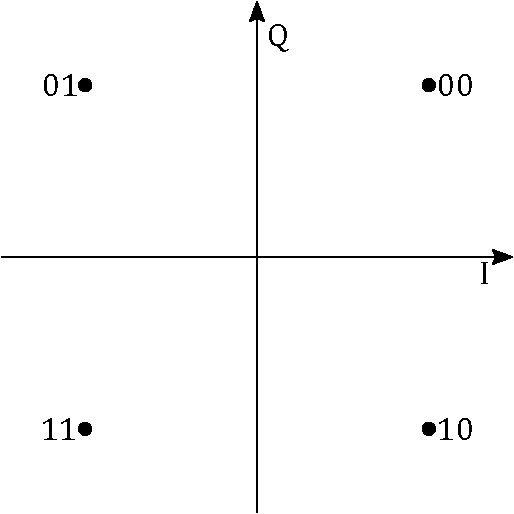
\includegraphics[width=0.5\textwidth]{./sdf/m_qam_system/figures/constellation.pdf}
	\caption{4-QAM constellation points.}
	\label{fig:const}
\end{figure}

%M can take several values: $2, 4, 16, 32, ...$. The first two correspond to BPSK and QPSK modulation, respectively.

\subsection{Theoretical Analysis}

M-QAM is a modulation scheme that takes advantage of two sinusoidal carriers with a phase difference of $\pi/2$. The resultant output consists of a signal with both amplitude and phase variations. The two carriers, referred to as I (In-phase) and Q (Quadrature), can be represented as

\begin{align}
	I(t)=A(t)\cos(\phi t) \\
	Q(t)=A(t)\sin(\phi t)
\end{align}
which means that any sinusoidal wave can be decomposed in its I and Q components:

\begin{align}
	A\cos(\omega~t+\phi)&=A\left(\cos(\omega~t)\cos(\phi)-\sin(\omega~t)\sin(\phi)\right) \\
	&=I\cos(\omega~t)-Q\sin(\omega~t),
\end{align}
where we have used the expression for the cosine of a sum and the definitions of I and Q.



For the particular case of $M=4$, considering there is no crosstalk or interference between the Q and I components, the signal can be treated as a pair of independent BPSK systems, one for the in-phase component and another for the quadrature component.
Using Gray coding, adjacent symbols differ by only one bit. As such, an error in a single component leads to a single bit error.
This means that the probability of an error in bit detection is independent among components, as there is no crosstalk or interference. That being the case, the bit error rate can be calculated for the BPSK case.

%Considering a signal with amplitude $A$ sampled at the signal peak with no inter-symbol interference, and affected by noise with variance $n_0/2$, the sampled value will be a Gaussian random variable with mean $\pm A$ and variance $n_0/2$. Thus, the probability of error is given by the probability that the value is affected by a deviation greater than $m$.

Let the $s(t)$ be the signal sampled at a given instant $t$ for either the in-phase or quadrature component, $A(t)$ be the component corresponding to the transmitted signal with value equal to $\pm A$, depending on whether the transmitted signal was 1 or 0, and $n(t)$ the component associated with the Gaussian white noise with variance $n_0/2$, such that

\begin{equation}\label{eq:sigAmpNoise}
s(t) = A(t) + n(t)
\end{equation}

\begin{figure}[H]
	\centering
	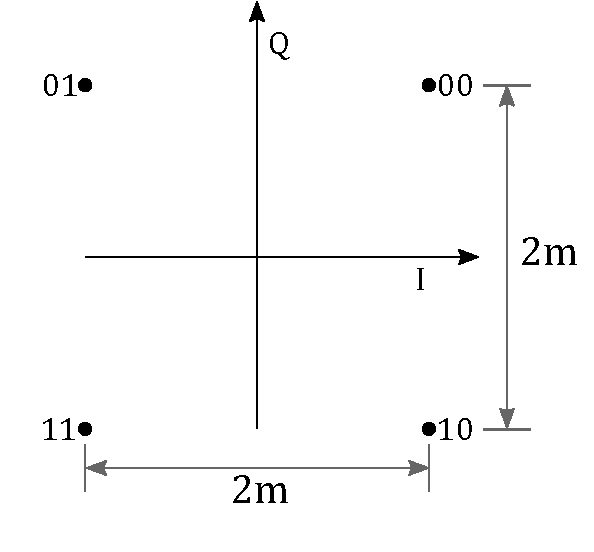
\includegraphics[width=0.5\textwidth]{./sdf/m_qam_system/figures/constellation_d.pdf}
	\caption{The relation between $m$ and the distance between constellation points.\label{fig:const_2m}}
\end{figure}

In this case, assuming the absence of inter-symbol interference, $s(t)$ will be a Gaussian random variable with average value of $\pm A$, depending on what signal was transmitted, and variance equal to $n_0/2$. In this case, using the constellation from Figure~\ref{fig:const_2m}, with a decision boundary halfway between $A$ and $-A$, an error occurs in two situations: when the a 0 is transmitted but a 1 is identified, or a 1 is transmitted and a 0 is identified. These mistakes happen when the perturbation in the signal due to noise is enough to push the value beyond the decision boundary. These situations are shown in Figures~\ref{fig:gauss} and~\ref{fig:gausserr}, by the colored area under the curve.

\begin{figure}[H]
	\centering
	\centering
	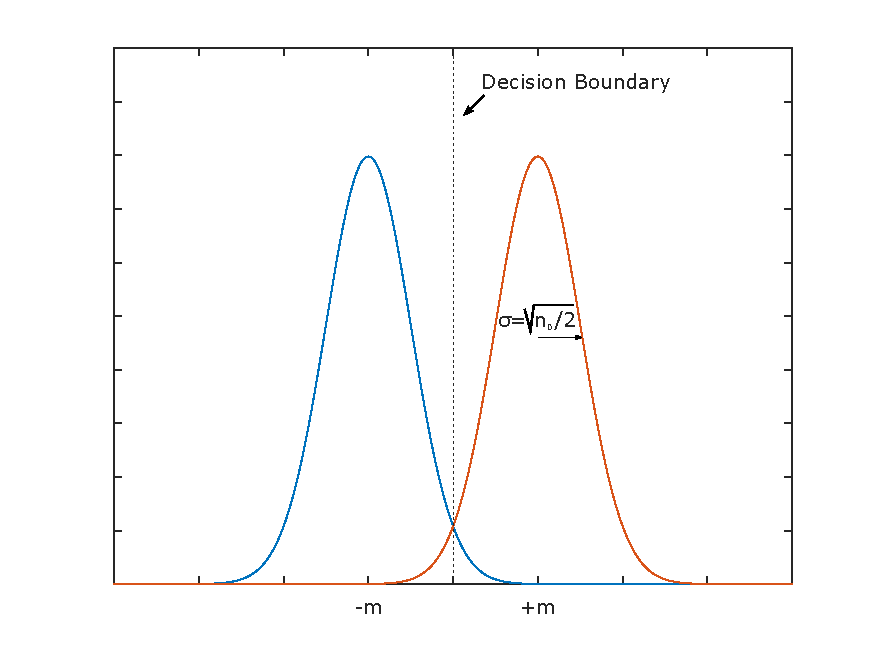
\includegraphics[ width=0.8\textwidth]{./sdf/m_qam_system/figures/gaussians.pdf}
	\caption{Probability density functions for $s(t) = m(t) + n(t)$, with $m(t)=\pm m$ and $n(t)$ as a Gaussian variable.}
	\label{fig:gauss}
\end{figure}

\begin{figure}[H]
	\centering
	\begin{subfigure}{.5\textwidth}
		\centering
		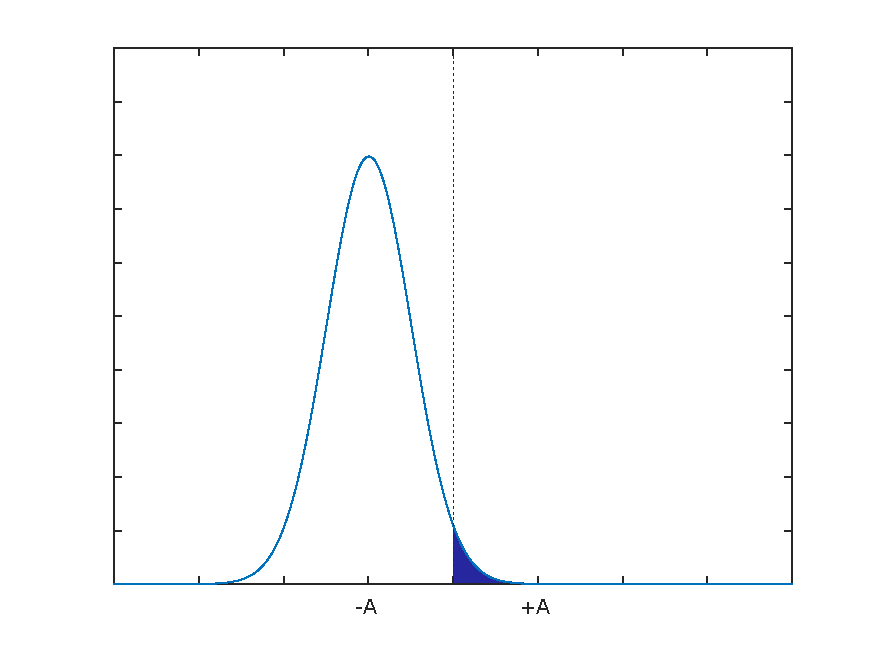
\includegraphics[clip, trim=1cm 0cm 1cm 0cm,width=\textwidth]{./sdf/m_qam_system/figures/gaussian_error_2.pdf}
	\end{subfigure}%
	\begin{subfigure}{.5\textwidth}
		\centering
		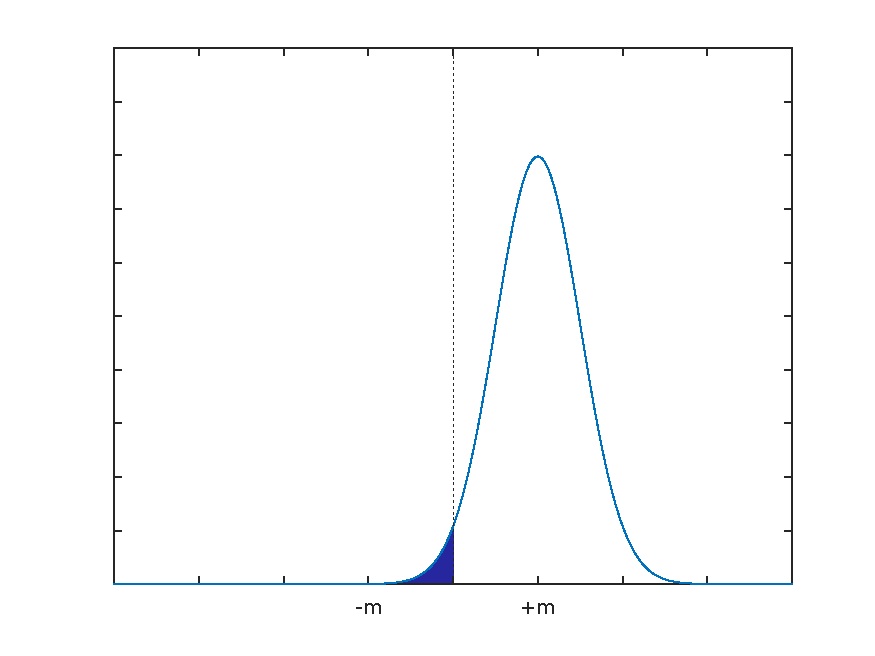
\includegraphics[clip, trim=1cm 0cm 1cm 0cm,width=\textwidth]{./sdf/m_qam_system/figures/gaussian_error.pdf}
	\end{subfigure}
	\caption{The area below the curves represents the probability of error for each transmitted bit.}
	\label{fig:gausserr}
\end{figure}

The probability of bit error can be expressed as:

\begin{equation}
P_{be} = P_0 P_{e0} + P_1 P_{e1}
\end{equation}

With equal probability for both bits, and considering the constellation's symmetry

\begin{equation}\label{eq:berMQAM}
P_{be} =  Q\left({\frac{A}{N}}\right) = \frac{1}{2} \text{erfc}\left({\frac{A}{\sqrt{2} N}}\right) = \frac{1}{2} \text{erfc}\left({\frac{A}{\sqrt{n_0}}}\right)
\end{equation}


%\begin{equation}
%P_b= Q\left(\sqrt{\frac{E_b}{n_0}}\right) = \frac{1}{2} erfc\left(\sqrt{\frac{E_b}{2 n_0}}\right).
%\end{equation}

%\begin{equation}\label{eq:berBPSK}
%P_{BE}= Q\left({\sqrt{\frac{2 E_b}{N_0}}}\right) = \frac{1}{2} \text{erfc}\left({\sqrt{\frac{ E_b}{N_0}}}\right).
%\end{equation}

%\begin{equation}\label{eq:berBPSK}
%BER= Q\left({G_{ele}\sqrt{\frac{2 P_L P_S}{n_0}}}\right) = \frac{1}{2} \text{erfc}\left({G_{ele}\sqrt{\frac{P_L P_S}{n_0}}}\right).
%\end{equation}

with


\begin{eqnarray}
&A &= G_{ele} \sqrt{P_L P_S}\label{eq:bpskamplitude}\\
&N &= \sqrt{\frac{n_0}{2}}
\end{eqnarray}
%\begin{equation}\label{eq:berBPSK}
%BER= Q\left({G_{ele}\sqrt{\frac{2 P_L P_S}{n_0}}}\right) = \frac{1}{2} \text{erfc}\left({G_{ele}\sqrt{\frac{P_L P_S}{n_0}}}\right).
%\end{equation}

\noindent where $P_L$ is the local oscillator power, $P_S$ is the average optical power of the laser source on which the signal is modulated, $G_{ele}$ is the gain in the transimpedance amplifier and $n_0$ is the noise spectral density. Figure~\ref{fig:const_2m} shows the relation between the constellation points and $A$. $N_0$ will be the standard deviation of the sampled values.





The symbol error rate however is not the same, as it depends on both bits being correctly detected. The probability of both bits being correctly detected is:

\begin{equation}
P_C = (1 - P_{be})^2
\end{equation}

From this, the probability of symbol error is:

\begin{eqnarray}
&P_s &= 1-P_C \nonumber\\
&	   &= 1 - \left(1 - Q \left({\frac{A}{n_0}}\right)\right)^2 \nonumber \\
&	   &= 2 Q\left({\frac{A}{n_0}}\right)\left[1-\frac{1}{2} Q \left({\frac{A}{n_0}}\right)\right]
\end{eqnarray}

%The bit error rate is then equal to the probability of the phase falling outside the correct detection range in a given component due to noise,


%Exact solutions for the probability of symbol and bit errors exist only for $M=4$.

%As previously mentioned, for $M=4$ the system is reduced to a QPSK system. Knowing that the AWGN is independent

%For the cases of $M>4$, an aproximation can be used.
%The probability of symbol error, $P_s$, in coherent M-PSK demodulation with AWGN can be aproximated by
%
%\begin{equation}
%	P_s=2~Q\left(\sqrt{2~\log_2 M \left(\frac{E_b}{n_0}\right)\sin^2\frac{\pi}{M}}\right)
%\end{equation}
%where $E_b$ is the energy of one bit, $n_0$ is the noise power and the function $Q$ is defined as
%\begin{equation}
%	Q(x)=\frac{1}{2} erfc\left(\frac{x}{\sqrt{2}}\right).
%	\label{eq:Ps}
%\end{equation}
%
%It is worth noting that this aproximation is only valid for high SNR values. The probability of bit errors for $M>4$ can now be estimated, as it is related to $P_s$ by
%
%\begin{equation}
%	P_b=\frac{1}{\log_2 M}P_s.
%	\label{eq:Pb}
%\end{equation}
%
%For QPSK we get, using $M=4$ in equations \ref{eq:Ps} and \ref{eq:Pb},
%\begin{equation}
%	P_b= 2 Q\left(\sqrt{\frac{2~E_b}{n_0}}\right) = erfc\left(\sqrt{\frac{E_b}{n_0}}\right).
%\end{equation}
%
%The exact probability bit error for $M=4$ are

%The Bit Error Rate curve given by~\eqref{eq:berBPSK} is plotted in figure \ref{fig:QPSK_th_curve} as a function of the optical signal power for $N_0=10^{-6}$, $P_L = 0~dBm$ and $G_{ele} = 10^3$.

%\begin{figure}[h]
%		\centering
%		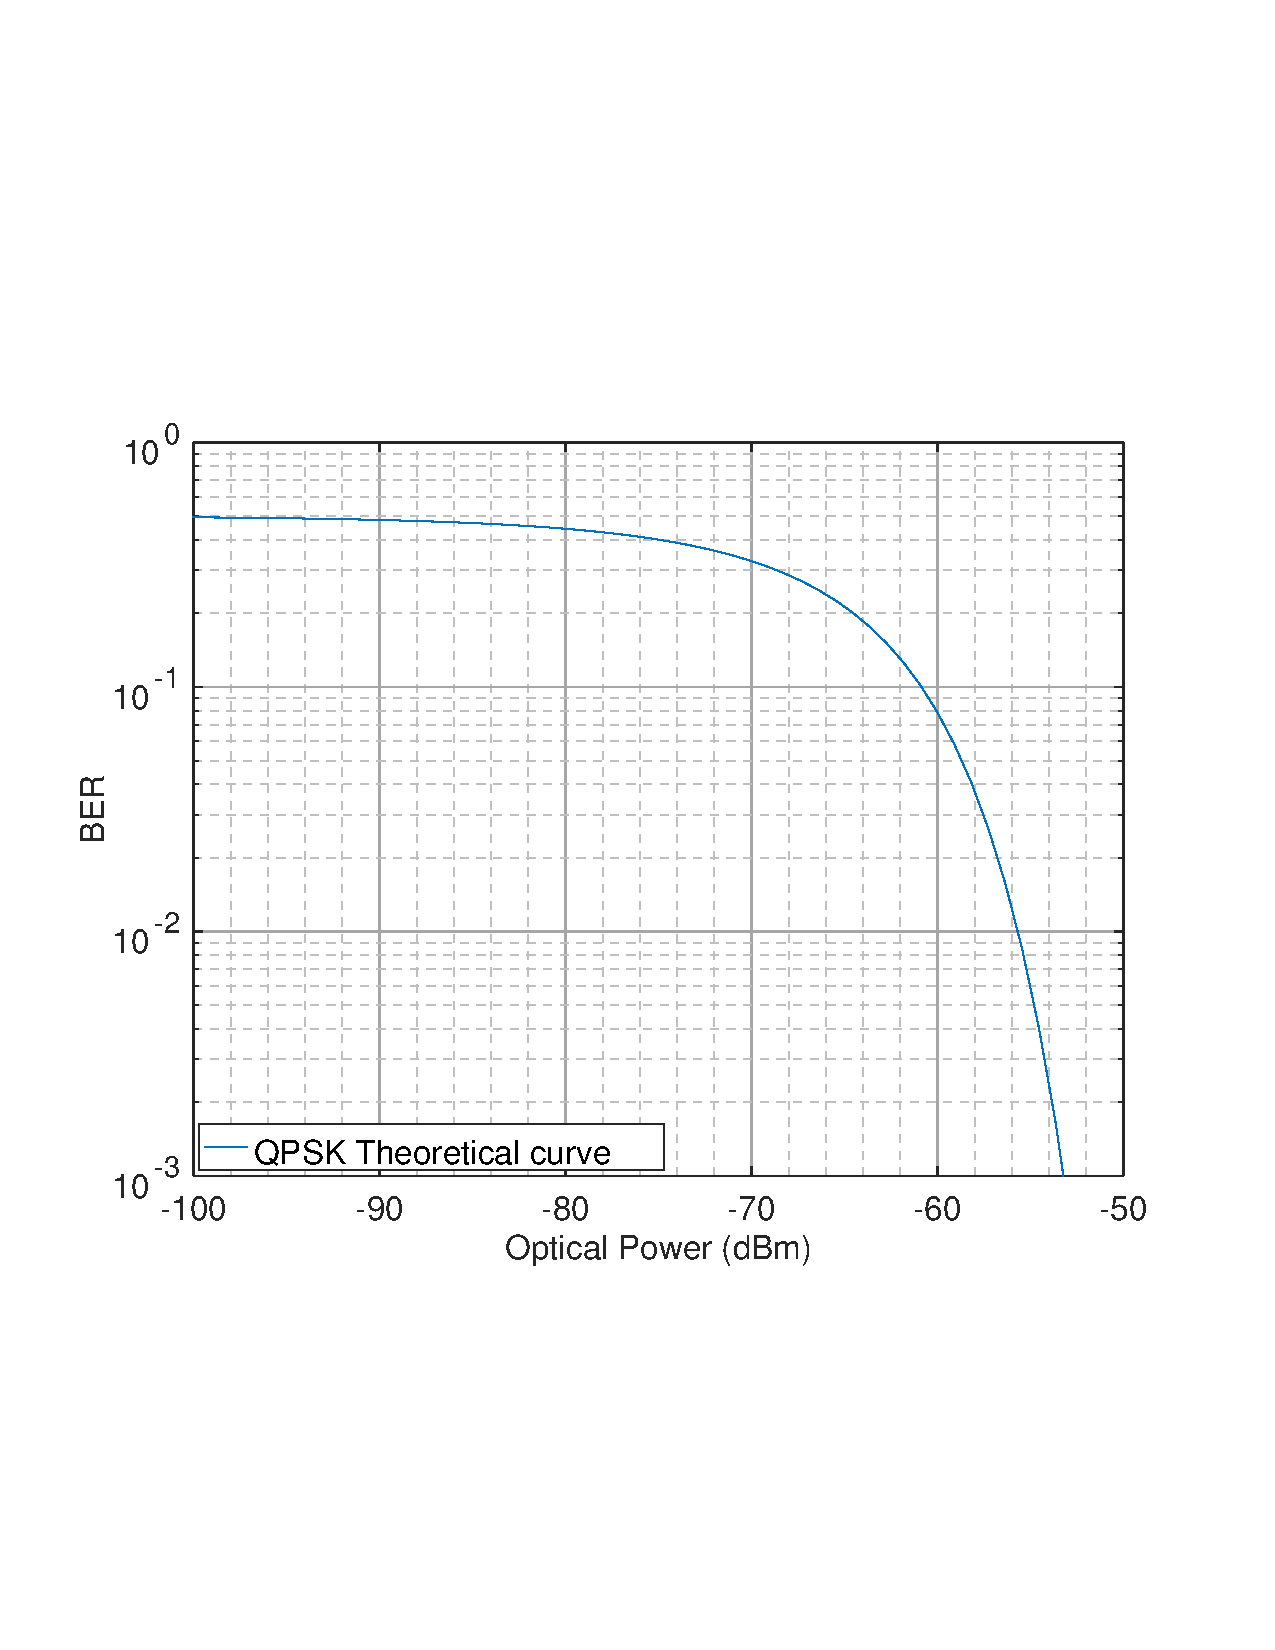
\includegraphics[clip, trim=2cm 6cm 2cm 6cm, width=0.7\textwidth]{./sdf/m_qam_system/figures/BER_QPSK_theory_20180119.pdf}
%		\caption{QPSK theoretical BER values as a function of the output optical power in dBm.}
%		\label{fig:QPSK_th_curve}
%\end{figure}

It is possible to further decrease the error rate by using a matched filter before sampling the signal. The resulting signal will still have Gaussian noise, but the signal-to-noise ratio will be greatly improved. This can be achieved by using a root-raised cosine filter at the pulse shaper and another one before the sampler. Inter-symbol interference will still be null as it is equivalent to a raised cosine filter, where half the filtering is done on the transmitter side (while pulse-shaping) and the other half is done on the receiver side, before sampling.

%As the constellation remains the same, the expression to calculate the BER is similar, but replacing the values of $m$ and $N_0$ of Equation~\eqref{eq:berMQAM} by those corresponding to the signal at the output of the filter, which can be calculated as:
Considering a signal similar to the one described by Equation~\ref{eq:sigAmpNoise}, the output of the matched filter receiver will be~\cite{mischasch}:

\begin{eqnarray}
&s_{mf} (t) &= \int_{0}^{T} s(t)\cos(\omega_0 t ) dt\nonumber\\ 
&	       &= \int_{0}^{T} m(t) \cos(\omega_0 t ) dt + \int_{0}^{T} n(t) \cos(\omega_{0} t ) dt
\end{eqnarray}

In the case of QPSK with m=4, both the quadrature and in-phase components have $m(t) = \pm A$. The values that replace $m$ and $N_0$ in Equation~\ref{eq:berMQAM} become:

\begin{eqnarray}
&A_{mf} &= \frac{A T}{2} = \frac{G_{ele} \sqrt{P_L P_S} T}{2}\\
&N_{mf} &= \sqrt{\sigma_o^2} = E(n_o^2) = \sqrt{\frac{n_0 T}{4}}
\end{eqnarray}

Here, $P_L$ is the local oscillator power, $P_S$ is the average optical power of the laser source on which the signal is modulated, $G_{ele}$ is the gain in the transimpedance amplifier, T is the symbol period, $A_mf$ is the average amplitude at the sampling points of the signal after amplification without noise, $\sigma_o^2$ is the variance of the noise component of the matched filter output, the and $n_0$ is the noise spectral density.


The optimal BER that can be obtained by using matched filtering is then given by:

\begin{eqnarray}\label{eq:berBPSK}
&P_{be} &= \frac{1}{2} Q\left({\frac{A_{mf}}{\sqrt{2} N_{mf}}}\right)\nonumber\\
&		&= \frac{1}{2} \text{erfc}\left({\frac{A_{mf}}{\sqrt{2} N_{mf}}}\right)\nonumber\\
&	    &= \frac{1}{2} \text{erfc}\left(\sqrt{{\frac{A^2T}{2 n_0}}}\right)\\
%&	    &= \frac{1}{2} \text{erfc}\left(\sqrt{{\frac{E_b}{n_0}}}\right)\nonumber
\end{eqnarray}

with

\begin{eqnarray}
&A &= G_{ele} \sqrt{P_L P_S}
%&m_{mf} &= \frac{1}{2} T G_{ele} \sqrt{P_L P_S} \\
%&E_b &= \frac{A^2 T}{2} \\
\end{eqnarray}


\noindent where T is the symbol period, A is as defined in Equation~\ref{eq:bpskamplitude}, the average peak amplitude of the signal without noise prior to filtering.
%and $B_e$ is the energy of a single received bit.

Figure~\ref{fig:QPSK_th_curves} show the curves for both these equations, in the case where  $n_0=10^{-6}$, $P_L = 0~dBm$ and $G_{ele} = 10^3$.
%Here, $T$ is the symbol period. 


\begin{figure}[H]
		\centering
		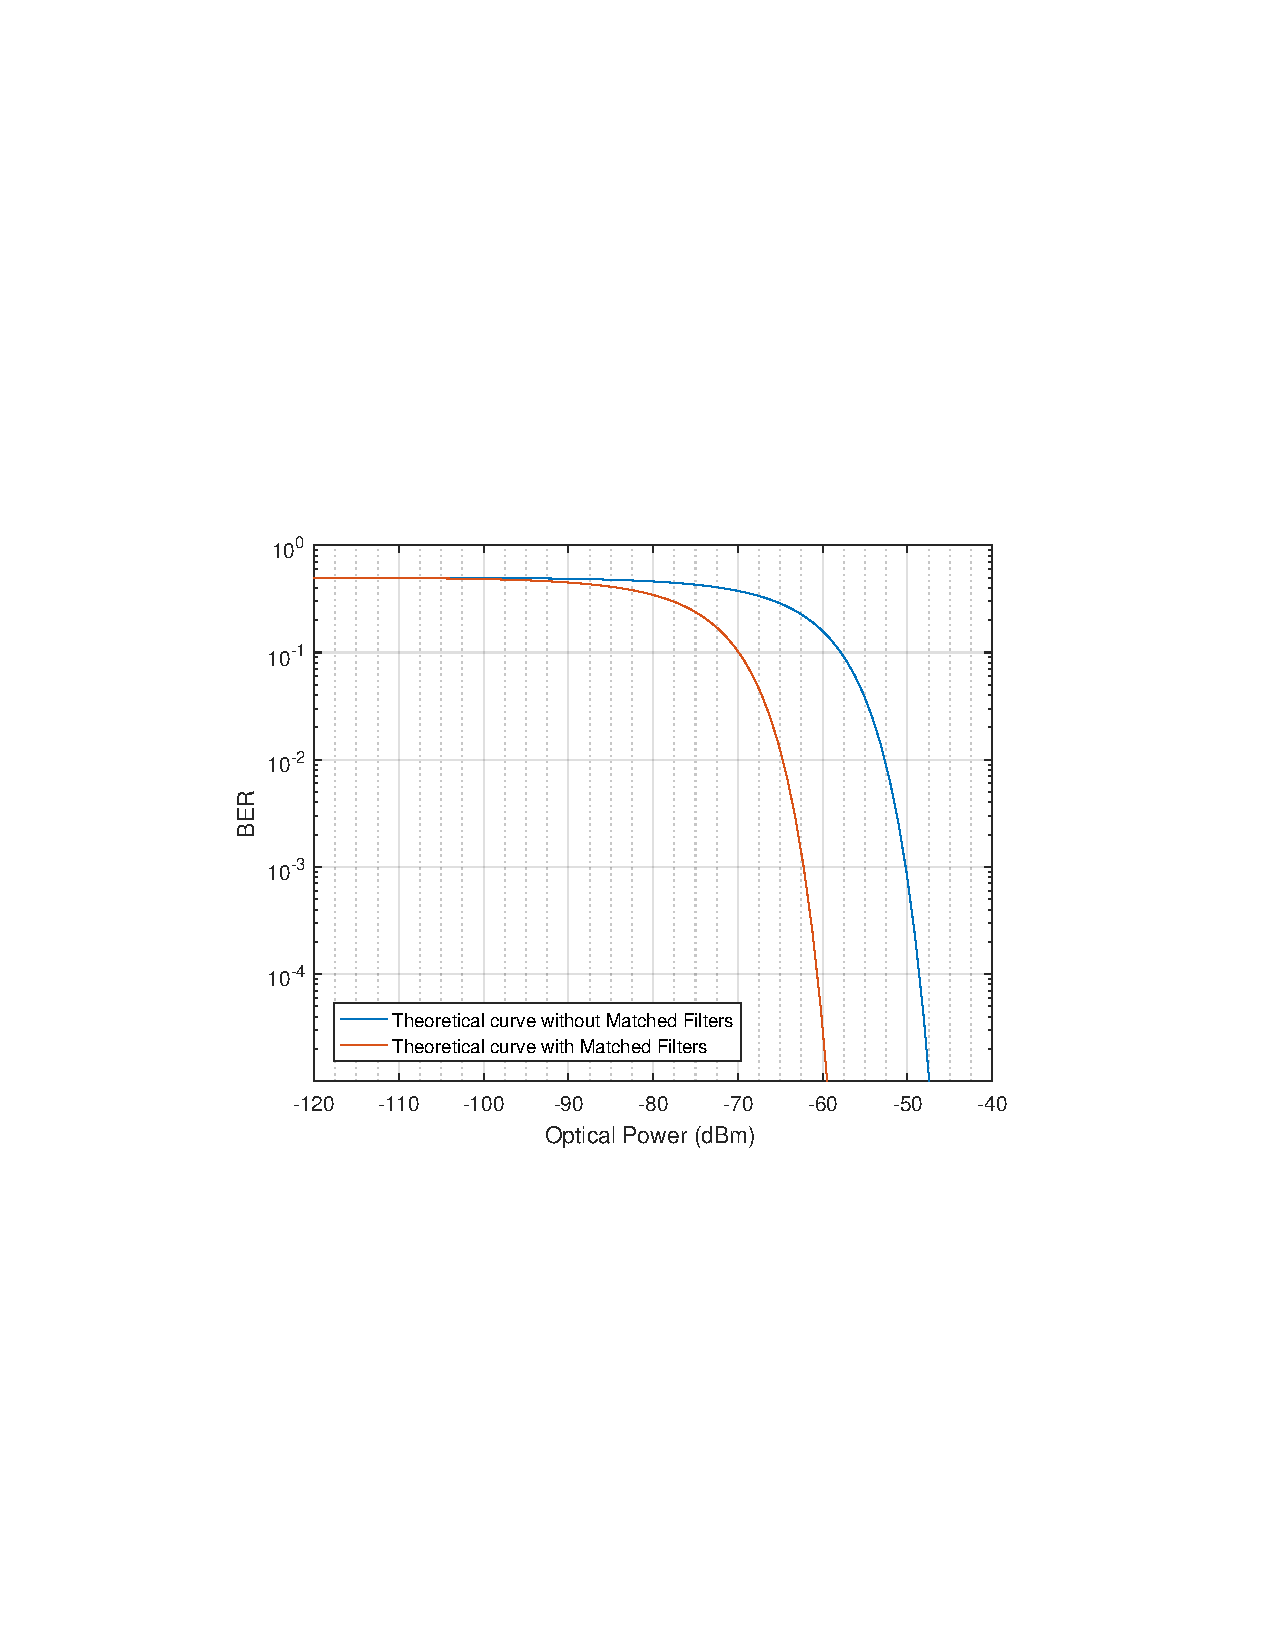
\includegraphics[clip, trim=4cm 8cm 4cm 8cm, width=0.7\textwidth]{./sdf/m_qam_system/figures/teor_BER_curves.pdf}
		\caption{QPSK theoretical BER values as a function of the output optical power in dBm.\label{fig:QPSK_th_curves}}	
\end{figure}

Figure~\ref{fig:QPSK_th_curves} shows the two theoretical curves for QPSK. The blue one is for QPSK without matched filtering and the red one is using root-raised-cosine for matched filtering, which provides optimum transmission. As the use of root-raised-cosine for matched filtering maximizes the signal-to-noise ratio to its optimal value, it allows achieving the same BER with much lower optical power. On the blue curve, on the other hand, the sampling is affected by the full effect of the random noise, as there is no filtering at the receiver. Because of this, a higher optical power is required to achieve a similar BER.


It's worth noting that these equations are only valid for M=4, as in that case the system is similar to QPSK with a 4 point constellation. For $M > 4$ a different approach is required.

The use of matched filtering should allow transmission with a lower SNR to achieve the same results as a similar system, even when using a shape with no inter-symbol interference. This is due to the second filter reducing the noise impact before detection, while not causing inter-symbol interference or degradation of the signal data.

\subsection{Simulation Analysis}

\begin{figure}[h]
	\centering
	
\includegraphics[width=0.8\textwidth]{./sdf/m_qam_system/figures/simulation_mqam}
	\caption{Schematic representation of the MQAM system.}\label{MQAM_system_block_diagram}
\end{figure}

The M-QAM transmission system is a complex block of code that simulates the modulation, transmission and
demodulation of an optical signal using M-QAM modulation.
It is composed of four blocks: a transmitter, a receiver, a sink and a block that performs a Bit Error Rate (BER) measurement. The schematic representation of the
system is presented in figure \ref{MQAM_system_block_diagram}.
	
\paragraph{Current state:} The system currently being implement is a QPSK system (M=4).

\paragraph{Future work:} Extend this block to include other values of M.

\subsection*{Functional description}

A complete description of the M-QAM transmitter and M-QAM homodyne receiver blocks can be found in the \textit{Library} chapter of this document as well as a detailed description of the independent blocks that compose these blocks.

The M-QAM transmitter generates one or two optical signals by encoding a binary string using M-QAM modulation. It also outputs a binary signal that is used to perform the BER measurement.

The M-QAM homodyne receiver accepts one input optical signal and outputs
a binary signal. It performs the M-QAM demodulation of the input signal by combining the optical signal with a local oscillator.

The demodulated optical signal is compared to the binary one produced by the transmitter in order to estimate the Bit Error Rate (BER).

The files used are summarized in tables~\ref{tab:sources} and~\ref{tab:headers}. These include all blocks and sub-blocks used and allow for the full operation of the M-QAM system.

\subsection*{Required files}\label{Required files}

\begin{table}[H]
    \centering
    \begin{tabulary}{1.0\textwidth}{|p{7.5cm}|p{5.5cm}|p{1cm}|}
        \hline
        \multicolumn{3}{|c|}{ \textbf{Source Files} } \\
        \hline
        \textbf{File}                      			 & \textbf{Comments} & \textbf{Status} \\ \hline
        add\_20171116.cpp                            &                   & \checkmark \\ \hline
        binary\_source\_20180118.cpp                 &                   & \checkmark \\ \hline
        bit\_error\_rate\_20171810.cpp               &                   & \checkmark \\ \hline
        decoder\_20180118.cpp                        &                   & \checkmark \\ \hline
        discrete\_to\_continuous\_time\_20180118.cpp &                   & \checkmark \\ \hline
        homodyne\_receiver\_20171203.cpp             & $^{1}$			 & \checkmark \\ \hline
        ideal\_amplififer\_20180118.cpp              &                   & \checkmark \\ \hline
        iq\_modulator\_20180118.cpp                  &                   & \checkmark \\ \hline
        local\_oscillator\_20180118.cpp              &                   & \checkmark \\ \hline
        m\_qam\_mapper\_20180118.cpp                 &                   & \checkmark \\ \hline
        m\_qam\_system.cpp                 			 & $^{2}$   		 & \checkmark \\ \hline
        m\_qam\_transmitter\_20180118.cpp            &                   & \checkmark \\ \hline
        netxpto\_20180118.cpp                        & $^{2}$ 			 & \checkmark \\ \hline
        optical\_hybrid\_20180118.cpp                &                   & \checkmark \\ \hline
        photodiode\_old\_20180118.cpp                &                   & \checkmark \\ \hline
        pulse\_shaper\_20180118.cpp                  &                   & \checkmark \\ \hline
        sampler\_20171119.cpp                        &                   & \checkmark \\ \hline
        sink\_20180118.cpp                           &                   & \checkmark \\ \hline
        super\_block\_interface\_20180118.cpp        & $^{2}$ 			 & \checkmark \\ \hline
        white\_noise\_20180118.cpp                   & 					 & \checkmark \\ \hline
    \end{tabulary}

    \caption{$^1$ The library entry is under a different name, \textit{m\_qam\_receiver};\\
    $^2$ No library entry as it is a main or general purpose file, not a specific block. 	 \label{tab:sources}}
\end{table}

\begin{table}[H]
    \centering
    \begin{tabulary}{1.0\textwidth}{|p{7cm}|p{6cm}|p{1cm}|}
        \hline
        \multicolumn{3}{|c|}{ \textbf{Header Files} } \\
        \hline
        \textbf{File}                      & \textbf{Comments} & \textbf{Status} \\ \hline
        add\_20171116.h                            & 			   & \checkmark \\ \hline
        binary\_source\_20180118 .h                &                   & \checkmark \\ \hline
        bit\_error\_rate\_20171810.h               &             & \checkmark \\ \hline
        decoder\_20180118.h                        &                   & \checkmark \\ \hline
        discrete\_to\_continuous\_time\_20180118.h &                   & \checkmark \\ \hline
        homodyne\_receiver\_20171203.h             & $^{1}$          & \checkmark \\ \hline
        ideal\_amplifier\_20180118.h               &                   & \checkmark \\ \hline
        iq\_modulator\_20180118.h                  &                   & \checkmark \\ \hline
        local\_oscillator\_20180118.h              &                   & \checkmark \\ \hline
        m\_qam\_mapper\_20180118.h                 &                   & \checkmark \\ \hline
        m\_qam\_transmitter\_20180118.h            &                   & \checkmark \\ \hline
        netxpto\_20180118.h                        & $^2$ 			   & \checkmark \\ \hline
        optical\_hybrid\_20180118.h                &                   & \checkmark \\ \hline
        photodiode\_old\_20180118.h                &                   & \checkmark \\ \hline
        pulse\_shaper\_20180118.h                  &                   & \checkmark \\ \hline
        sampler\_20171119.h                        &               & \checkmark \\ \hline
        sink\_20180118.h                           &                   & \checkmark \\ \hline
        super\_block\_interface\_20180118.h        & $^2$			   & \checkmark \\ \hline
        white\_noise\_20180118.h                   &                   & \checkmark \\ \hline
    \end{tabulary}
    \caption{$^1$ The library entry is under a different name, \textit{m\_qam\_receiver}\\
    $^2$ No library entry as it is a main or general purpose file, not a specific block. \label{tab:headers}}
\end{table}

%\begin{table}[]
%	\centering
%	\caption{Main system files}
%	\begin{tabular}{|c|c|c|c|ccc}
%		\cline{1-4}
%		\textbf{System blocks} & \textbf{Source file} & \textbf{Header file}  &  \textbf{Status} & \\ \cline{1-4}
%		Main & m\_qam\_system\_sdf.cpp & --- & \checkmark & \\ \cline{1-4}
%		M-QAM transmitter & m\_qam\_transmitter\_20180118.cpp & m\_qam\_transmitter\_20180118.h & \checkmark &  \\ \cline{1-4}
%		M-QAM receiver & homodyne\_receiver\_20180118.cpp & homodyne\_receiver\_20180118.h & \checkmark &  \\ \cline{1-4}
%		Sink & sink\_20180118.cpp & sink\_20180118.h &  \checkmark & \\ \cline{1-4}
%		BER estimator & bit\_error\_rate\_20171810.cpp & bit\_error\_rate\_20171810.h & \checkmark &\\ \cline{1-4}
%	\end{tabular}
%	\label{files_table}
%\end{table}

%\subsection*{Required Files}
%
%The required header and source files needed to run this system are summarized in table \ref{table:files}.
%
%\begin{table}
% 	\centering
% 	\caption{Required files}
% 	\begin{tabular}{|c|c|p{40mm}|c|ccp{40mm}c}
% 		\cline{1-4}
% 		\textbf{Header file} & \textbf{Source file} & \textbf{Description} &  \textbf{Status} & \\ \cline{1-4}
% 		add.h & add.cpp & Adds two signals.  & \checkmark &   \\ \cline{1-4}
% 		binary\_source.h & binary\_source.cpp & Produces a binary sequence. & \checkmark & \\ \cline{1-4}
% 		bit\_error\_rate.h & bit\_error\_rate.cpp & Computes the BER and writes it to a text file. & \checkmark & \\ \cline{1-4}
% 		discrete\_to\_continuous\_time.h & discrete\_to\_continuous\_time.cpp & Converts a signal from discrete in time to continuous in time. & \checkmark & \\ \cline{1-4}
% 		homodyne\_receiver.h & m\_qam\_homodyne\_receiver.cpp & & \\ \cline{1-4}
% 		ideal\_amplifier.h & ideal\_amplifier.cpp & Amplifies the signal. & \checkmark & \\ \cline{1-4}
% 		iq\_modulator.h & iq\_modulator.cpp & Divides the signal in its quadrature and in phase components & \checkmark &\\ \cline{1-4}
% 		local\_oscillator.h & local\_oscillator.cpp & & & \checkmark &\\ \cline{1-4}
% 		m\_qam\_mapper.h & m\_qam\_mapper.cpp & Maps the signal using the defined constellation & \checkmark & \\ \cline{1-4}
% 		m\_qam\_transmitter.h & m\_qam\_transmitter.cpp & & \checkmark & \\ \cline{1-4}
% 		netxpto.h & netxpto.cpp & General class that contains definition from signals and buffers. & \checkmark &\\ \cline{1-4}
% 		optical\_hybrid.h & optical\_hybrid.cpp & Implements an optical hybrid. & \checkmark & \\ \cline{1-4}
% 		photodiode\_old.h & photodiode\_old.cpp & Pair of photodiodes and current subtraction. & \checkmark & \\ \cline{1-4}
% 		pulse\_shaper.h & pulse\_shaper.cpp & Electrical filter. & \checkmark &\\ \cline{1-4}
% 		sampler\_20171119.h & sampler\_20171119.cpp & Samples the signal. & \checkmark &\\ \cline{1-4}
% 		sink.h & sink.cpp & Deletes signal. & \checkmark & \\ \cline{1-4}
% 		super\_block\_interface.h & super\_block\_interface.cpp & & \checkmark &\\ \cline{1-4}
% 		white\_noise.h & white\_noise.cpp & Generates white gaussian noise. & \checkmark &\\ \cline{1-4}
% 	\end{tabular}
% 	\label{table:files}
%\end{table}
\pagebreak
\subsection*{Input Parameters}

%The system accepts several input parameters that can be defined by the user. These are described in table \ref{table:in_par}.

\begin{table}[H]
	\centering
	\caption{Input parameters}
	\begin{tabular}{|c|c|p{70mm}|ccp{70mm}}
		\cline{1-3}
		\textbf{Parameter} & \textbf{Type} & \textbf{Description} &    \\ \cline{1-3}
		numberOfBitsGenerated & t\_integer & Determines the number of bits to be generated by the binary source  &    \\ \cline{1-3}
		samplesPerSymbol & t\_integer & Number of samples per symbol &    \\ \cline{1-3}
		prbsPatternLength & int & Determines the length of the pseudorandom sequence pattern (used only when the binary source is operated in \textit{PseudoRandom} mode) &    \\ \cline{1-3}
		bitPeriod & t\_real & Temporal interval occupied by one bit &    \\ \cline{1-3}
		rollOffFactor\_shp & t\_real & Parameter of the pulse shaper filter &    \\ \cline{1-3}
		rollOffFactor\_out & t\_real & Parameter of the output filter &    \\ \cline{1-3}
		shaperFilter & enum & Type of filter used in Pulse Shaper &    \\ \cline{1-3}
		outputFilter & enum & Type of filter used in output filter &    \\ \cline{1-3}
		seedType & enum & Method of seeding noise generators &    \\ \cline{1-3}
		seedArray & array<int,2> & Seeds to initialize noise generators &    \\ \cline{1-3}
		signalOutputPower\_dBm & t\_real & Determines the power of the output optical signal in dBm &  \\ \cline{1-3}
		numberOfBitsReceived & int &   Determines when the simulation should stop. If $-1$ then it only stops when there is no more bits to be sent&   \\ \cline{1-3}
		iqAmplitudeValues & vector<t\_iqValues> & Determines the constellation used to encode the signal in IQ space &    \\ \cline{1-3}
		symbolPeriod & double & Given by bitPeriod/samplesPerSymbol &    \\ \cline{1-3}
		localOscillatorPower\_dBm & t\_real & Power of the local oscillator &    \\ \cline{1-3}
		responsivity & t\_real & Responsivity of the photodiodes (1 corresponds to having all optical power transformed into electrical current) &    \\ \cline{1-3}
		amplification & t\_real & Amplification provided by the ideal amplifier &    \\ \cline{1-3}
		noiseAmplitude & t\_real & Amplitude of the white noise &    \\ \cline{1-3}
		samplesToSkip & t\_integer & Number of samples to be skipped by the \textit{sampler} block &    \\ \cline{1-3}
		confidence & t\_real & Determines the confidence limits for the BER estimation &    \\ \cline{1-3}
		midReportSize & t\_integer &  &    \\ \cline{1-3}
		bufferLength & t\_integer & Corresponds to the number of samples that can be processed in each run of the system &    \\ \cline{1-3}
		\end{tabular}
		\label{table:in_par}
		\end{table}

\subsection*{Simulation results}

In this section we show results obtained through the simulations. The
following sections show the eye diagrams of the signal obtained at three
different points in the system: the optical signal S1, the signals after
amplifying the electrical signal and adding the Gaussian white noise HMD12 and
HMD13, and the signal after the filter in the receiver. These eye diagrams will
be shown for a variety of system configurations, with varying noise and
filters, displaying the advantages of using matched filtering with an optimal
filter.

\subsubsection{Inter-symbol Interference}

These section presents the mentioned eye diagrams in configurations without any
noise added to the signal. This allows studying the effects of inter-symbol
interference caused only by the filters used at the pulse-shaper and at the
receiver, 

Figure~\ref{fig:eyespower} shows the eye diagrams for the S1 optical signals
for two different values of the output optical power. These were obtained using
a
raised-cosine filter as a pulse shaper, with a roll-off factor of 0.9. It can
be seen that no inter-symbol interference is present.

\begin{figure}[H]
	\centering
	\begin{subfigure}{.5\textwidth}
		\centering
		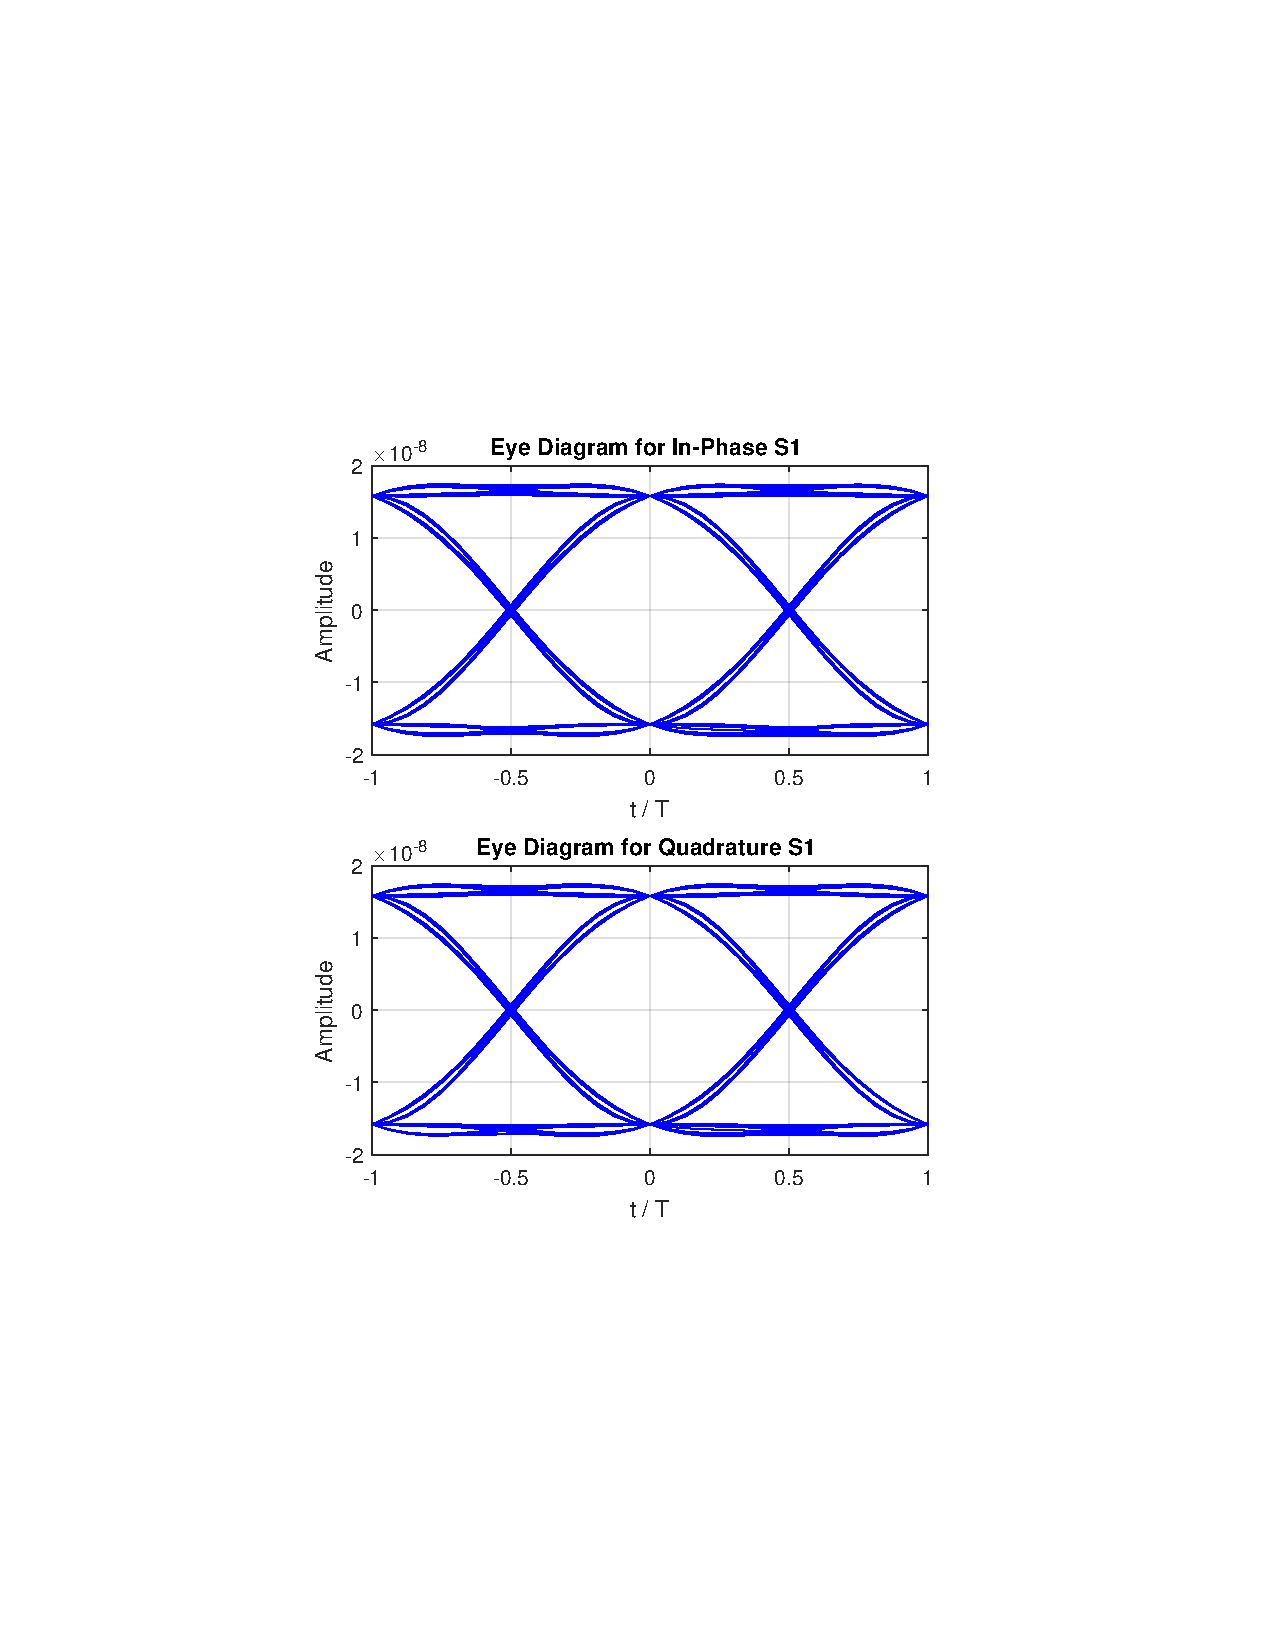
\includegraphics[clip, trim=5cm 7cm 5cm 7cm,
			width=\textwidth]{./sdf/m_qam_system/figures/eye120db09ro.pdf}
	\end{subfigure}%
	\begin{subfigure}{.5\textwidth}
		\centering
		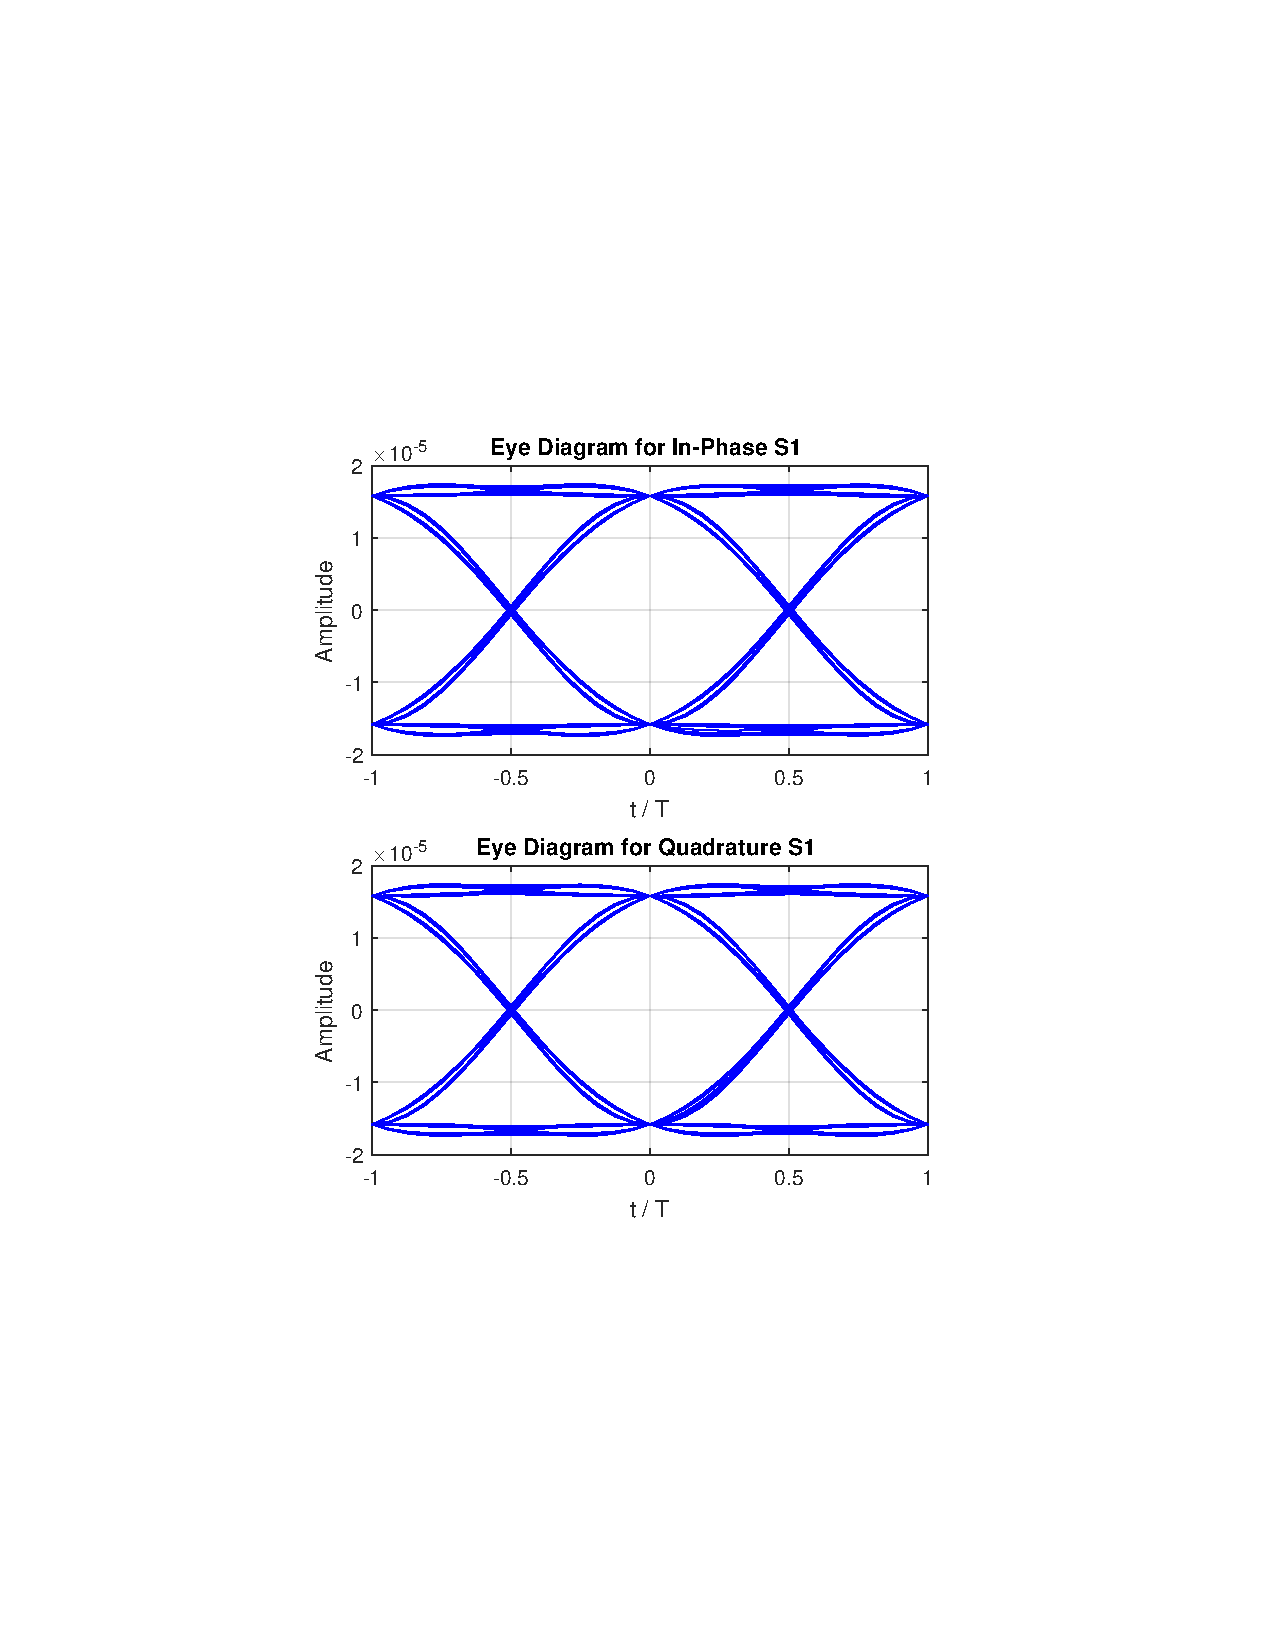
\includegraphics[clip, trim=5cm 7cm 5cm 7cm,
			width=\textwidth]{./sdf/m_qam_system/figures/eye60db09ro.pdf}
	\end{subfigure}
	\caption{Eye diagrams for the S1 bandpass signal with an output optical power
		of $-120$dBm (left) and $-60$dBm (right) with no added noise.}
	\label{fig:eyespower}
\end{figure}

As mentioned previously, using matched filters in highly beneficial, as it
allows achieving much lower error rates with the same optical power.

Figure~\ref{fig:eyes_nn_rc_09} shows the eye diagrams of the signal at the
three mentioned points, for a system without any added white noise, while using
matched filtering. The filter used in this case is a raised cosine filter with
a roll-off factor of 0.9. Although this is the ideal filter to use for pulse
shaping, as it does not cause inter-symbol-interference, it can be seen that
when used twice its results are less than ideal, as shown in the eye diagram
captured after the second filter.

\begin{figure}[H]
	\centering
	\begin{subfigure}{.45\textwidth}
		\centering
		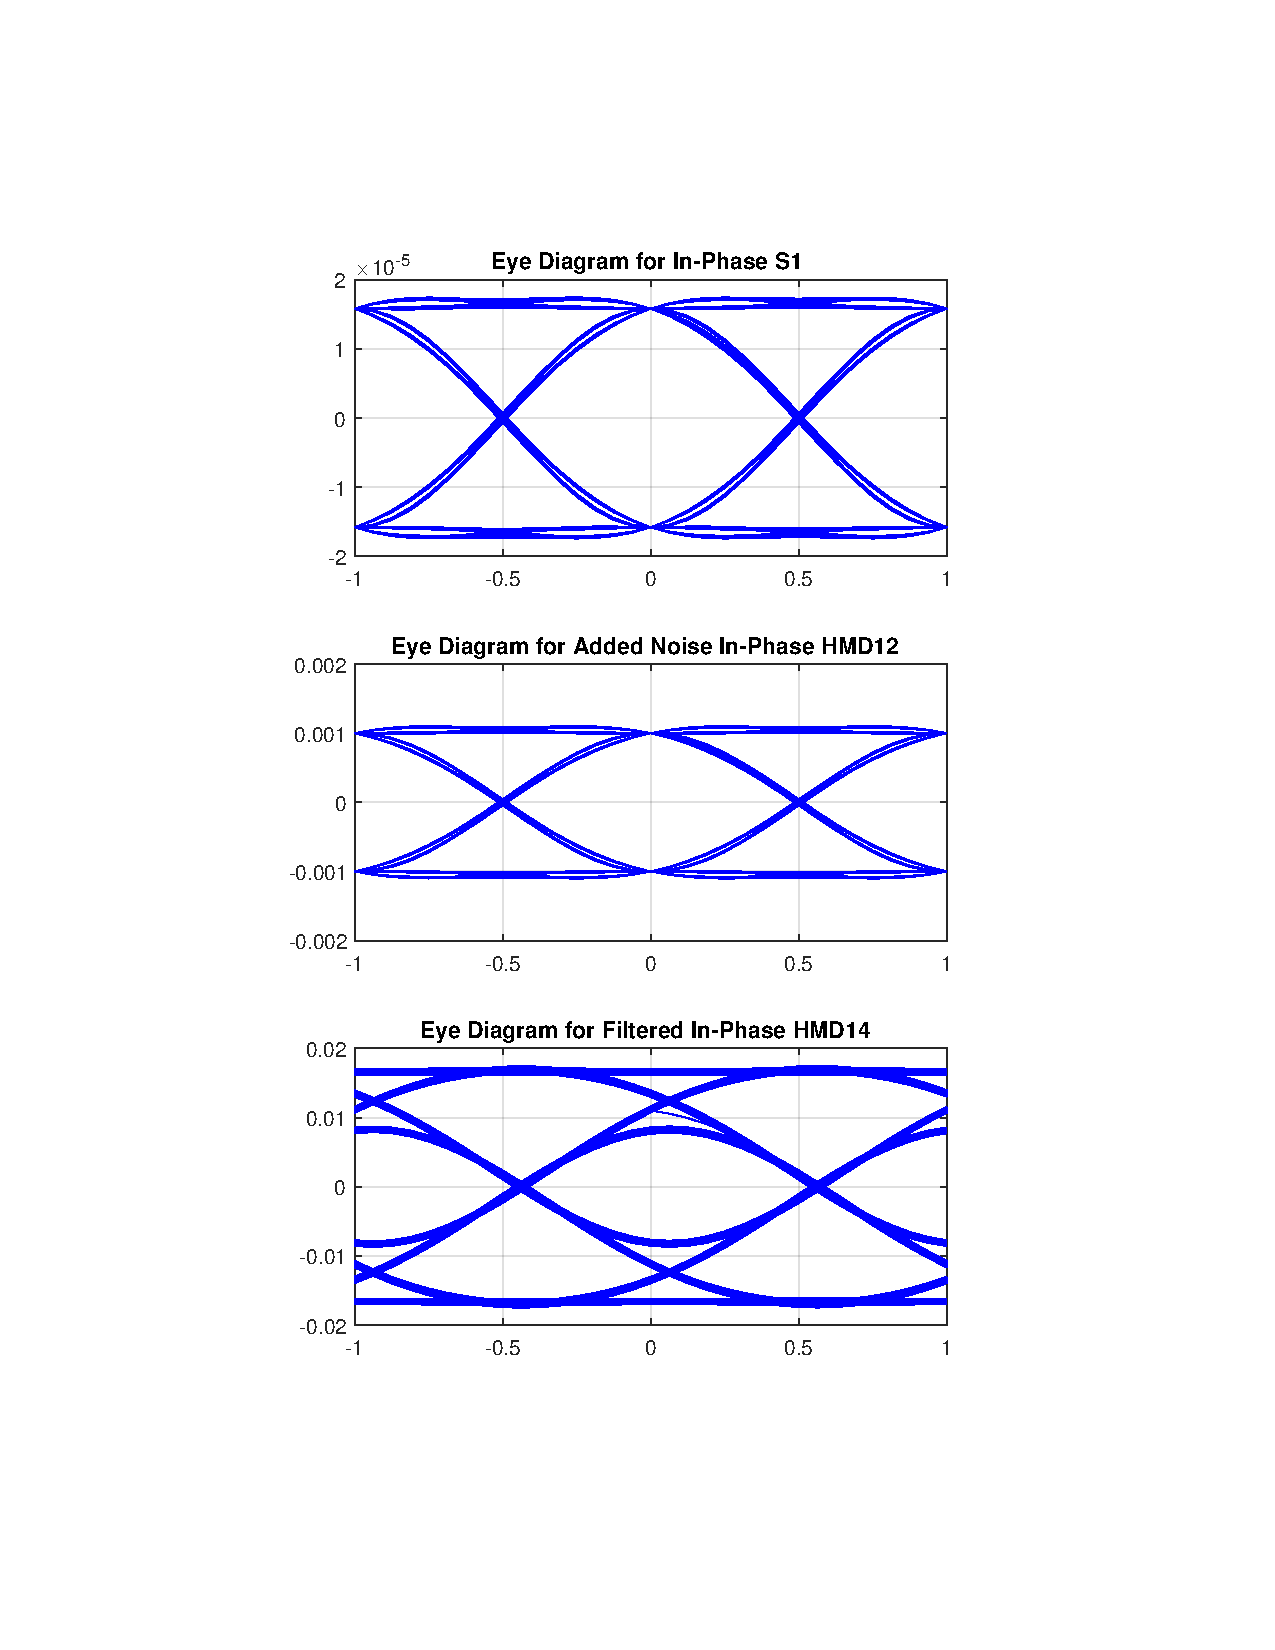
\includegraphics[clip, trim=5cm 4cm 5cm 4cm,
			width=\textwidth]{./sdf/m_qam_system/figures/eyes/if_nn_p_60_09_rc.pdf}
	\end{subfigure}
	\begin{subfigure}{.45\textwidth}
		\centering
		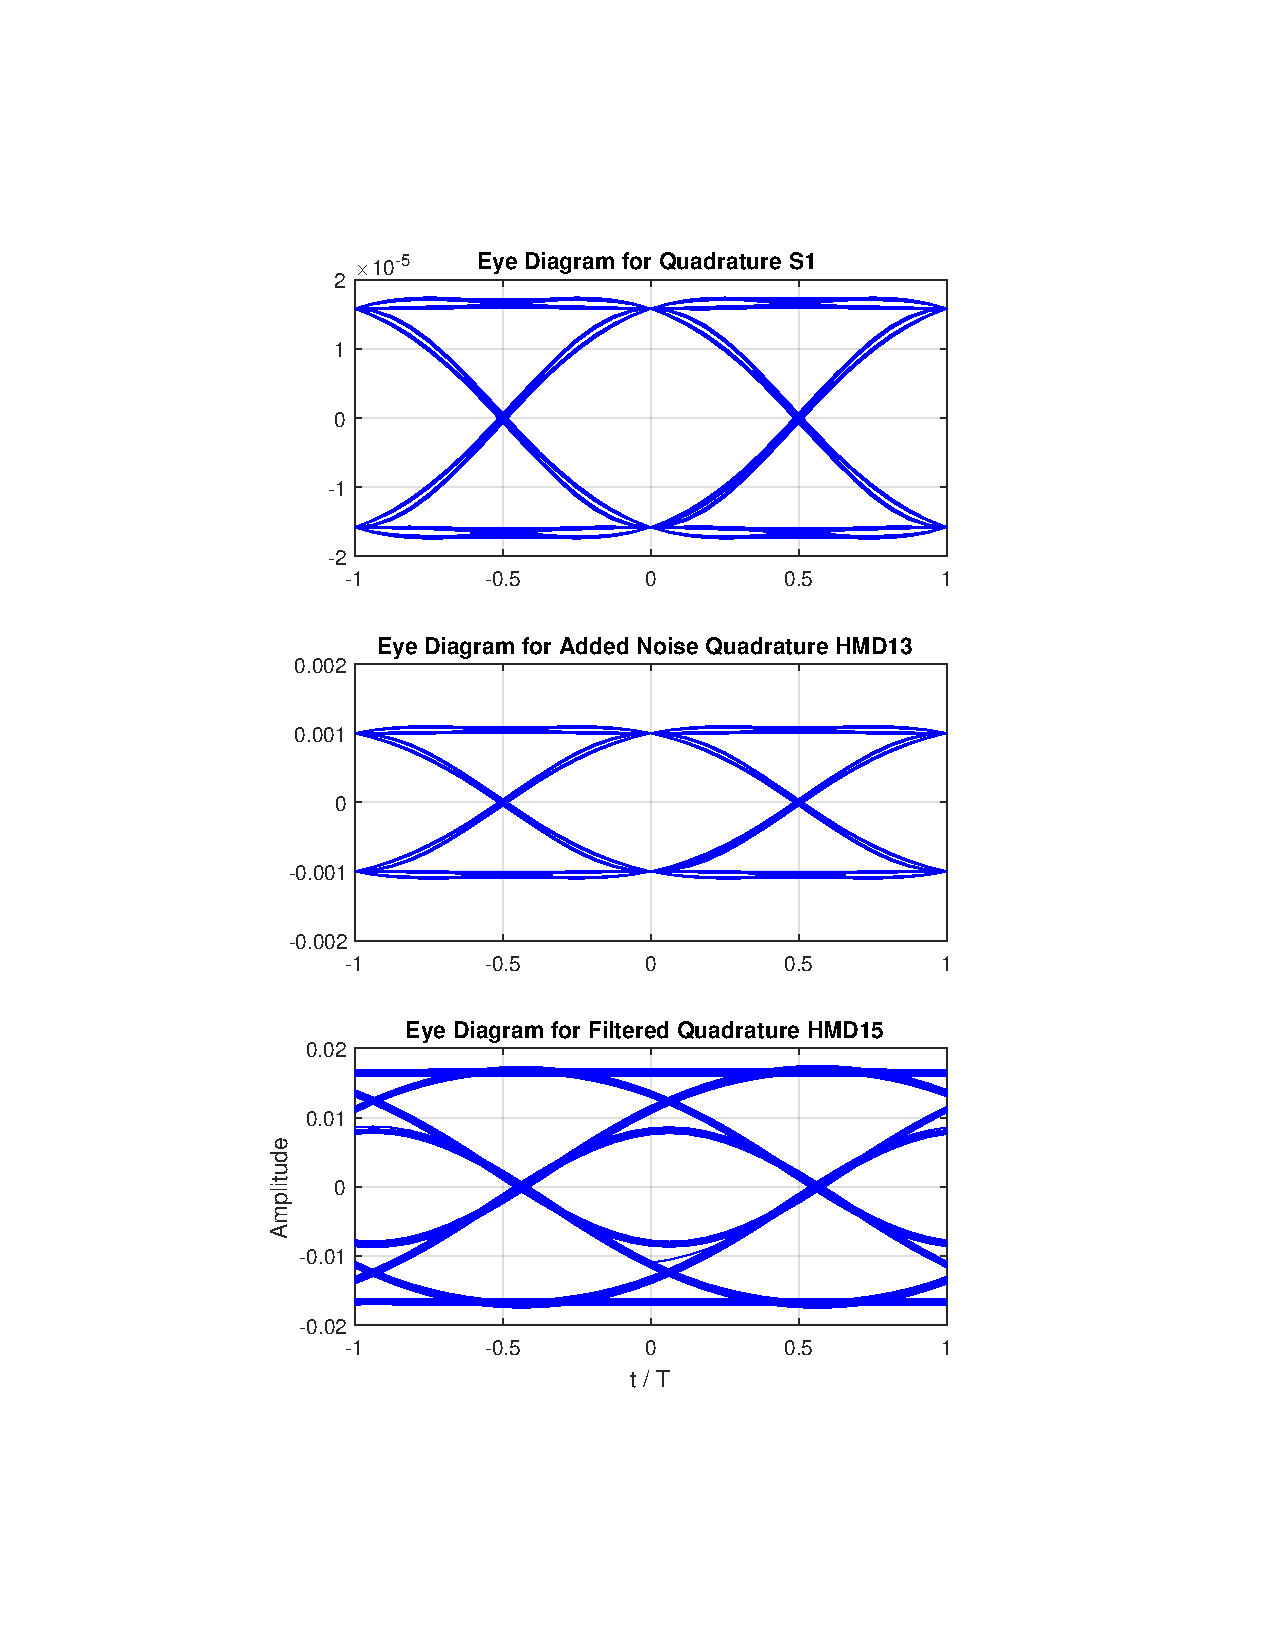
\includegraphics[clip, trim=5cm 4cm 5cm 4cm,
			width=\textwidth]{./sdf/m_qam_system/figures/eyes/q_nn_p_60_09_rc.pdf}
	\end{subfigure}
	
	\caption{Eye diagrams using matched filtering with raised-cosine at
		three different points, without AWGN: the optical output signal S1 on the top;
		the amplified signal at the middle, HMD12 and HMD13 for both components; and
		after passing through the last root-raised-cosine filter, HMD14 and HMD15, for
		both components. Obtained through simulation with an optical power output of
		-60 dBm, 0 dBm at the local oscillator, a gain of $10^3$ at the amplifier, and
		a rolloff factor of 0.9.\label{fig:eyes_nn_rc_09}}
	
\end{figure}

The optimum solution to achieving no inter-symbol interference while using
matched filtering is to use a root-raised-cosine to do the pulse-shaping at the
transmitter and the filtering at the receiver. The corresponding output of
applying twice a root-raised-cosine is exactly the same as using a
raised-cosine once. As such, the end result suffers from no inter-symbol
interference while reaping the benefits of optimum matched filtering.
Figure~\ref{fig:eyes_nn_rrc_09} shows the eye diagrams when using
root-raised-cosine filter both in the transmitter's pulse-shaper and at the
receiver's filter. The roll-off factor used in both was 0.9. It can be seen
that the shape of the eye diagram is equal to that of
Figure~\ref{fig:eyespower}, which uses a single raised cosine filter at the
pulse-shaper. Thus, it shows no sign of inter-symbol interference.

\begin{figure}[H]
	\centering
	\begin{subfigure}{.45\textwidth}
		\centering
		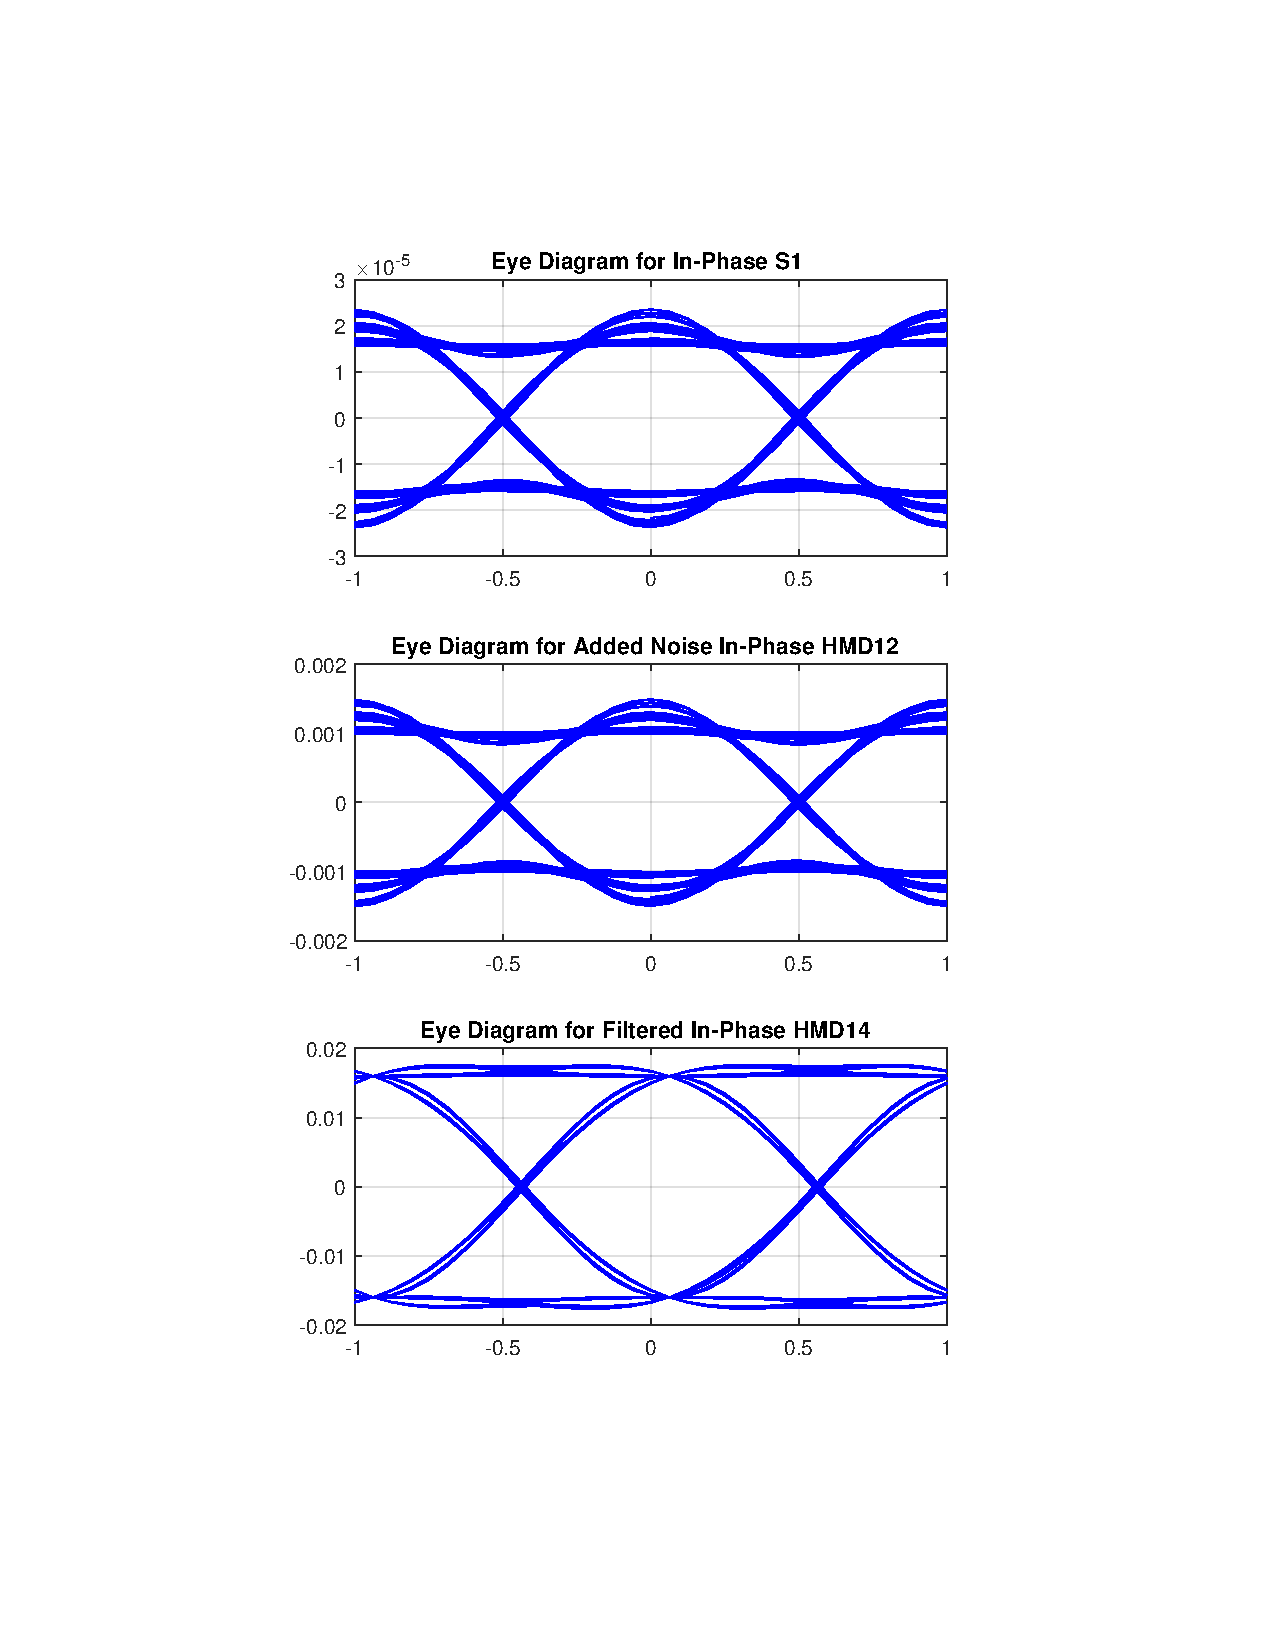
\includegraphics[clip, trim=5cm 4cm 5cm 4cm,
			width=\textwidth]{./sdf/m_qam_system/figures/eyes/if_nn_p_60_09.pdf}
	\end{subfigure}
	\begin{subfigure}{.45\textwidth}
		\centering
		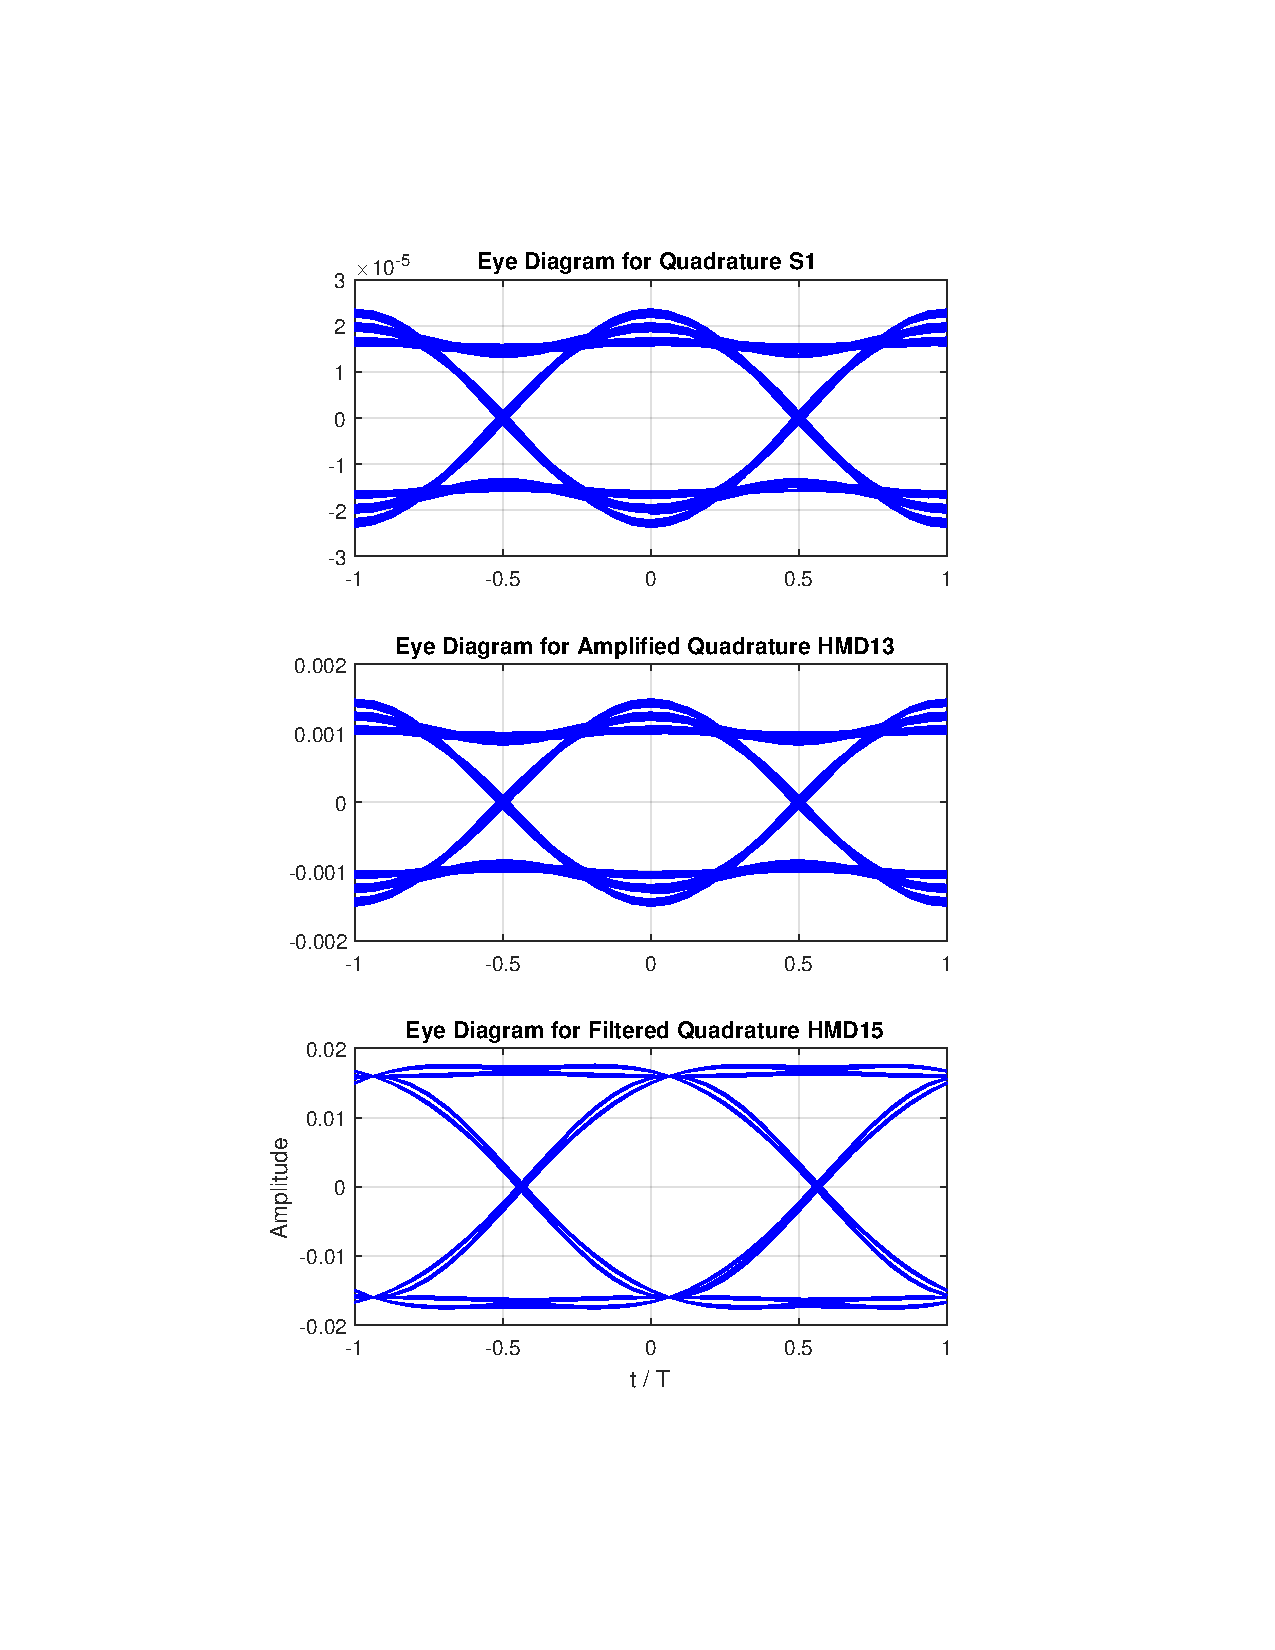
\includegraphics[clip, trim=5cm 4cm 5cm 4cm,
			width=\textwidth]{./sdf/m_qam_system/figures/eyes/q_nn_p_60_09.pdf}
	\end{subfigure}
	\caption{Eye diagrams using matched filtering with root-raised-cosine
		at three different points, without AWGN: the optical output signal S1 on the
		top; the amplified signal at the middle, HMD12 and HMD13 for both components;
		and after passing through the last root-raised-cosine filter, HMD14 and HMD15,
		for both components. Obtained through simulation with an optical power output
		of -60 dBm, 0 dBm at the local oscillator, a gain of $10^3$ at the amplifier,
		and a rolloff factor of 0.9.\label{fig:eyes_nn_rrc_09}}
	
\end{figure}

Figures~\ref{fig:eyes_nn_rrc_03} and~\ref{fig:eyes_nn_rrc_03} show a similar
comparison between matched filtering using raised-cosine or root-raised-cosine
filters, but with a roll-off factor of 0.3. Again, it can be seen that the
final shape of the eye diagram when using the root-raised-cosine for matched
filtering is the same as the shape of the optical signal S1 when using a
raised-cosine-filter.

\begin{figure}[H]
	\centering
	\begin{subfigure}{.45\textwidth}
		\centering
		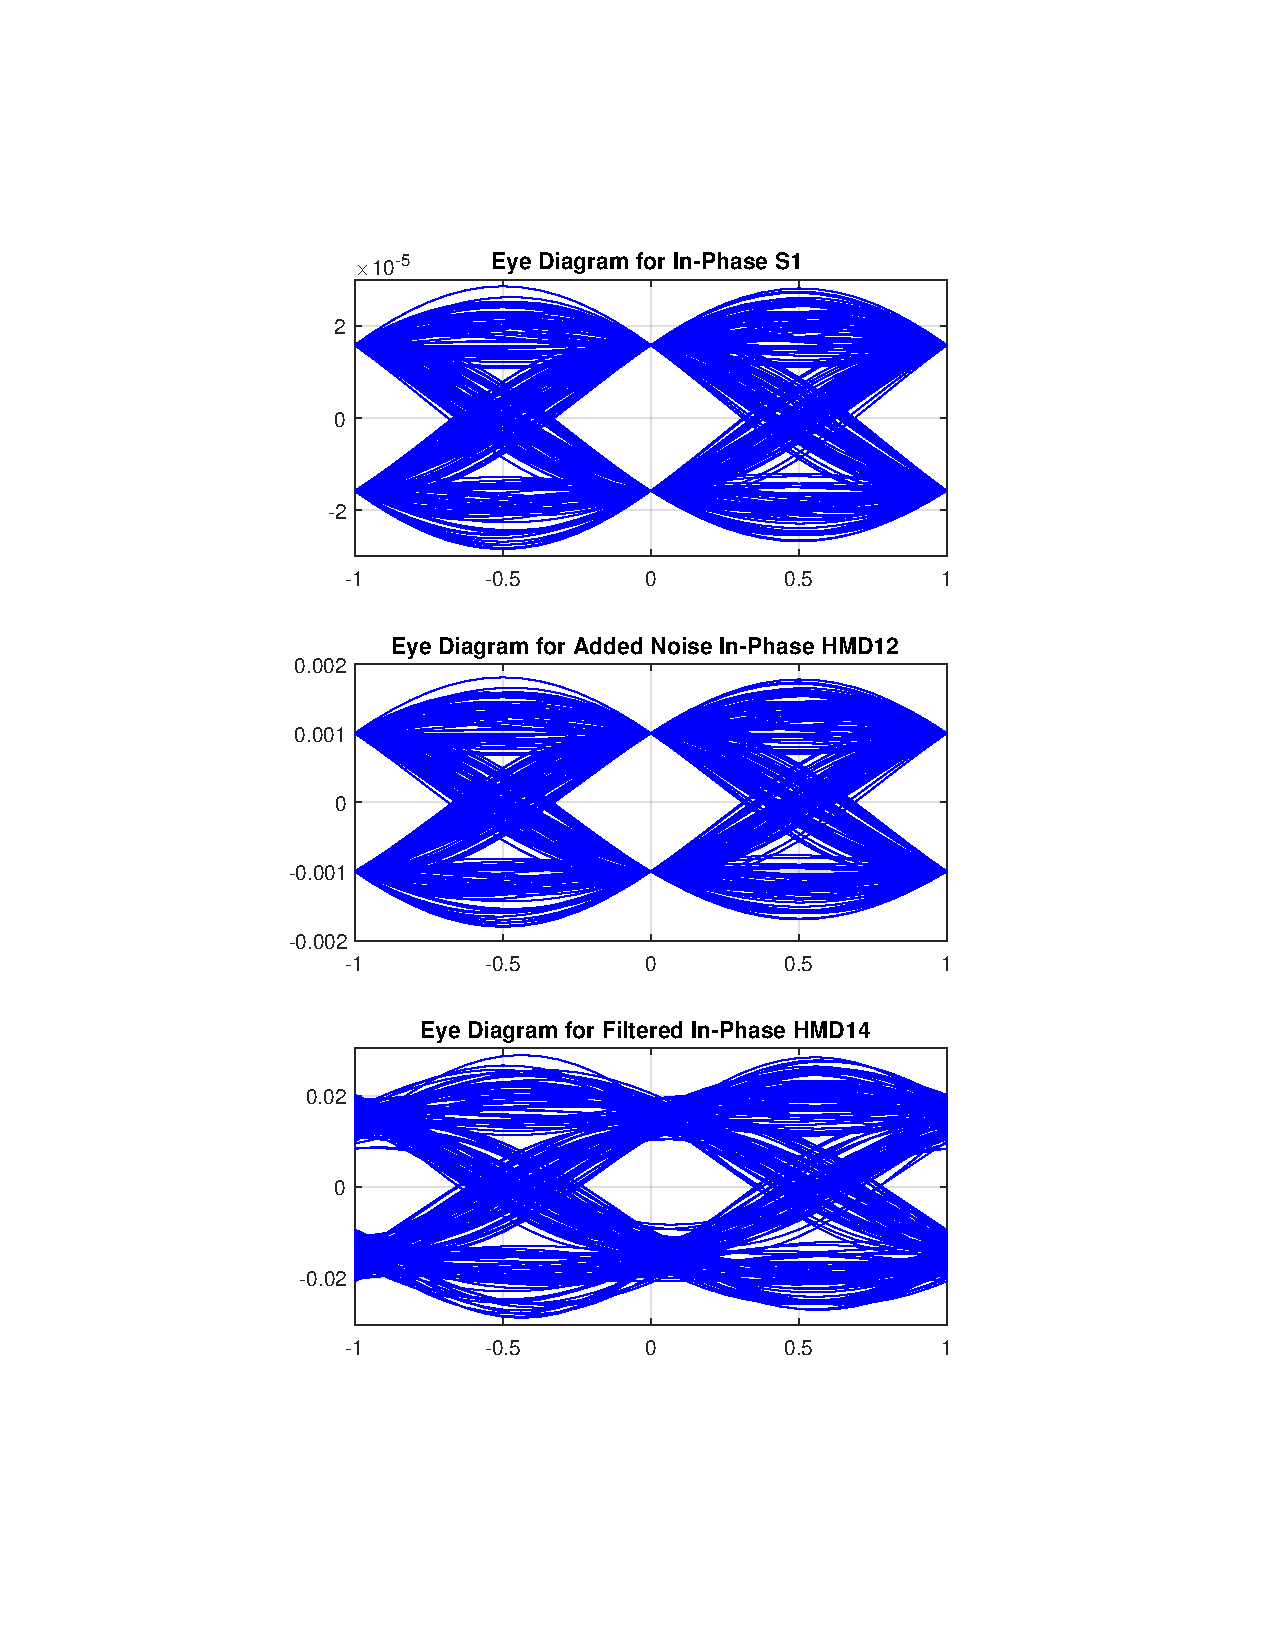
\includegraphics[clip, trim=5cm 4cm 5cm 4cm,
			width=\textwidth]{./sdf/m_qam_system/figures/eyes/if_nn_p_60_03_rc.pdf}
	\end{subfigure}
	\begin{subfigure}{.45\textwidth}
		\centering
		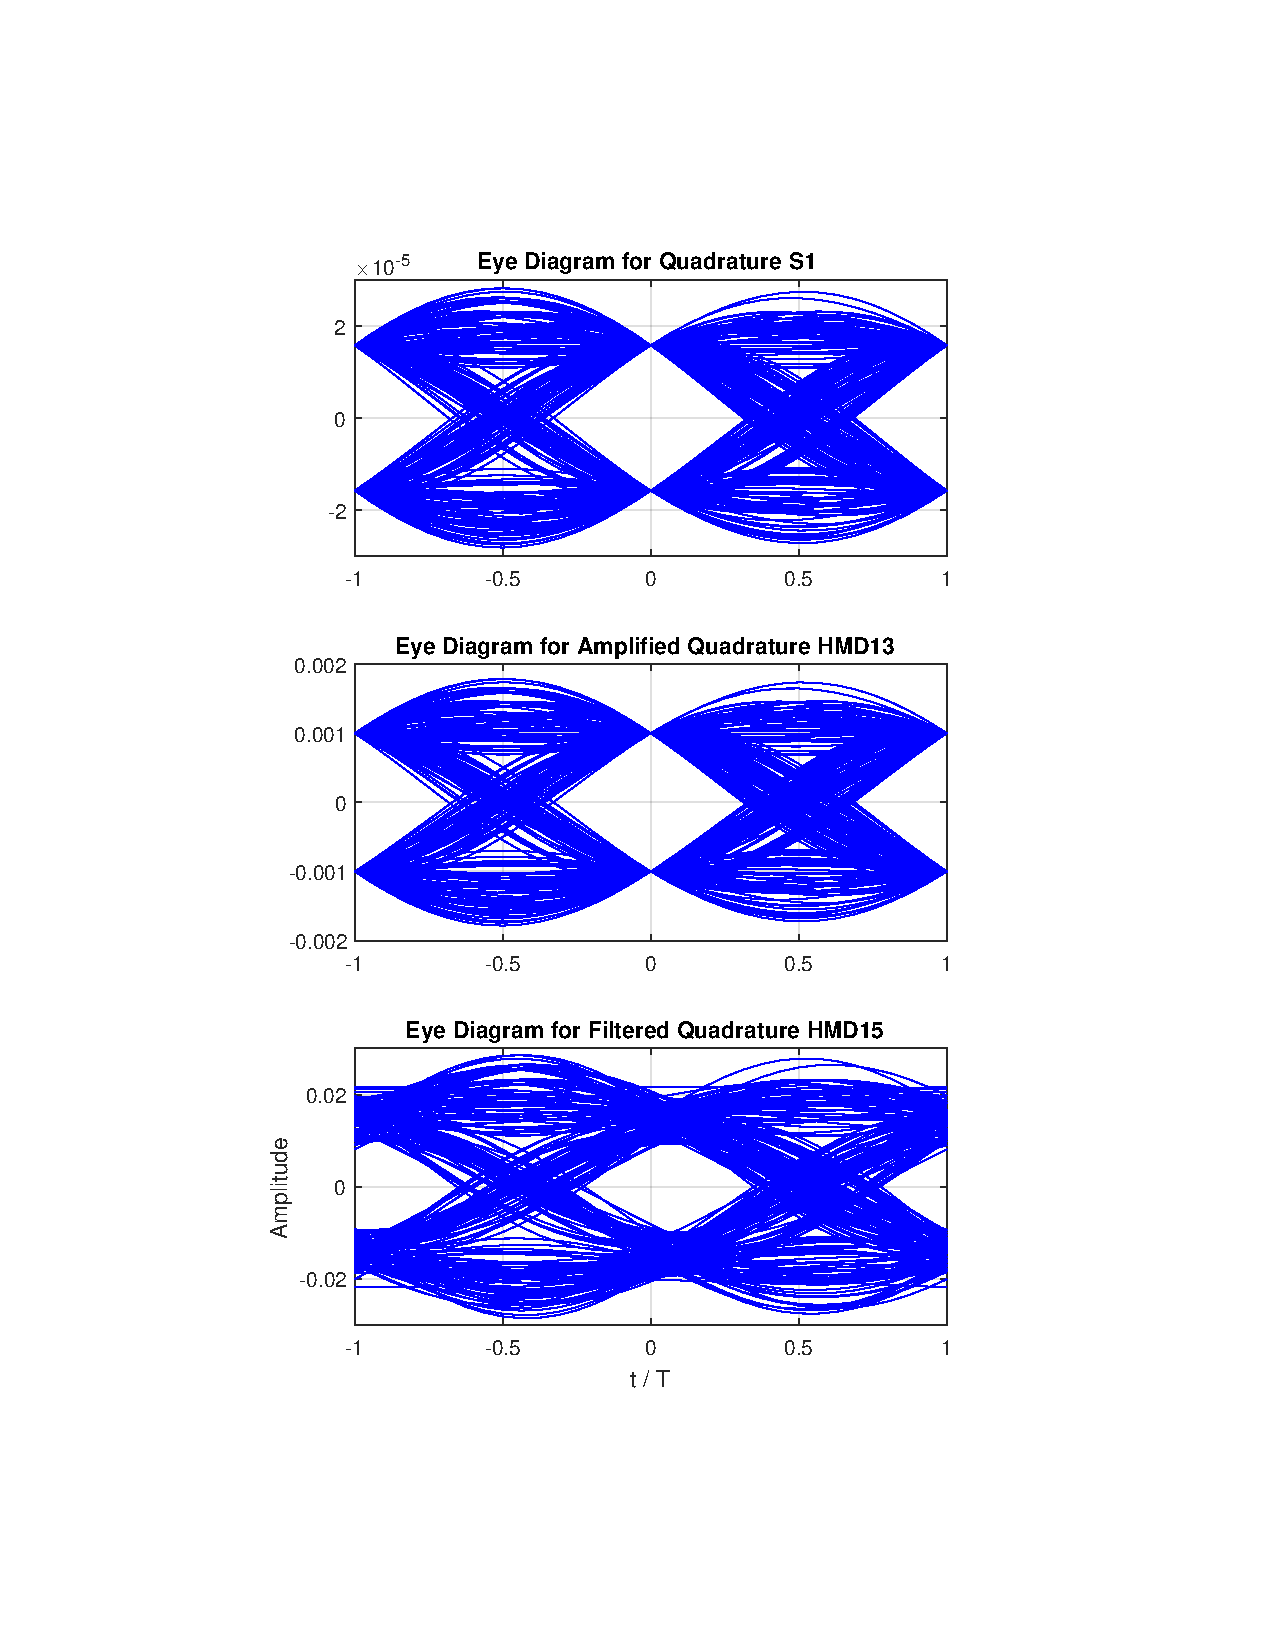
\includegraphics[clip, trim=5cm 4cm 5cm 4cm,
			width=\textwidth]{./sdf/m_qam_system/figures/eyes/q_nn_p_60_03_rc.pdf}
	\end{subfigure}
	
	\caption{Eye diagrams using matched filtering with raised-cosine at
		three different points, without AWGN: the optical output signal S1 on the top;
		the amplified signal at the middle, HMD12 and HMD13 for both components; and
		after passing through the last root-raised-cosine filter, HMD14 and HMD15, for
		both components. Obtained through simulation with an optical power output of
		-60 dBm, 0 dBm at the local oscillator, a gain of $10^3$ at the amplifier, and
		a rolloff factor of 0.3.\label{fig:eyes_nn_rc_03}}
	
\end{figure}


\begin{figure}[H]
	\centering
	\begin{subfigure}{.45\textwidth}
		\centering
		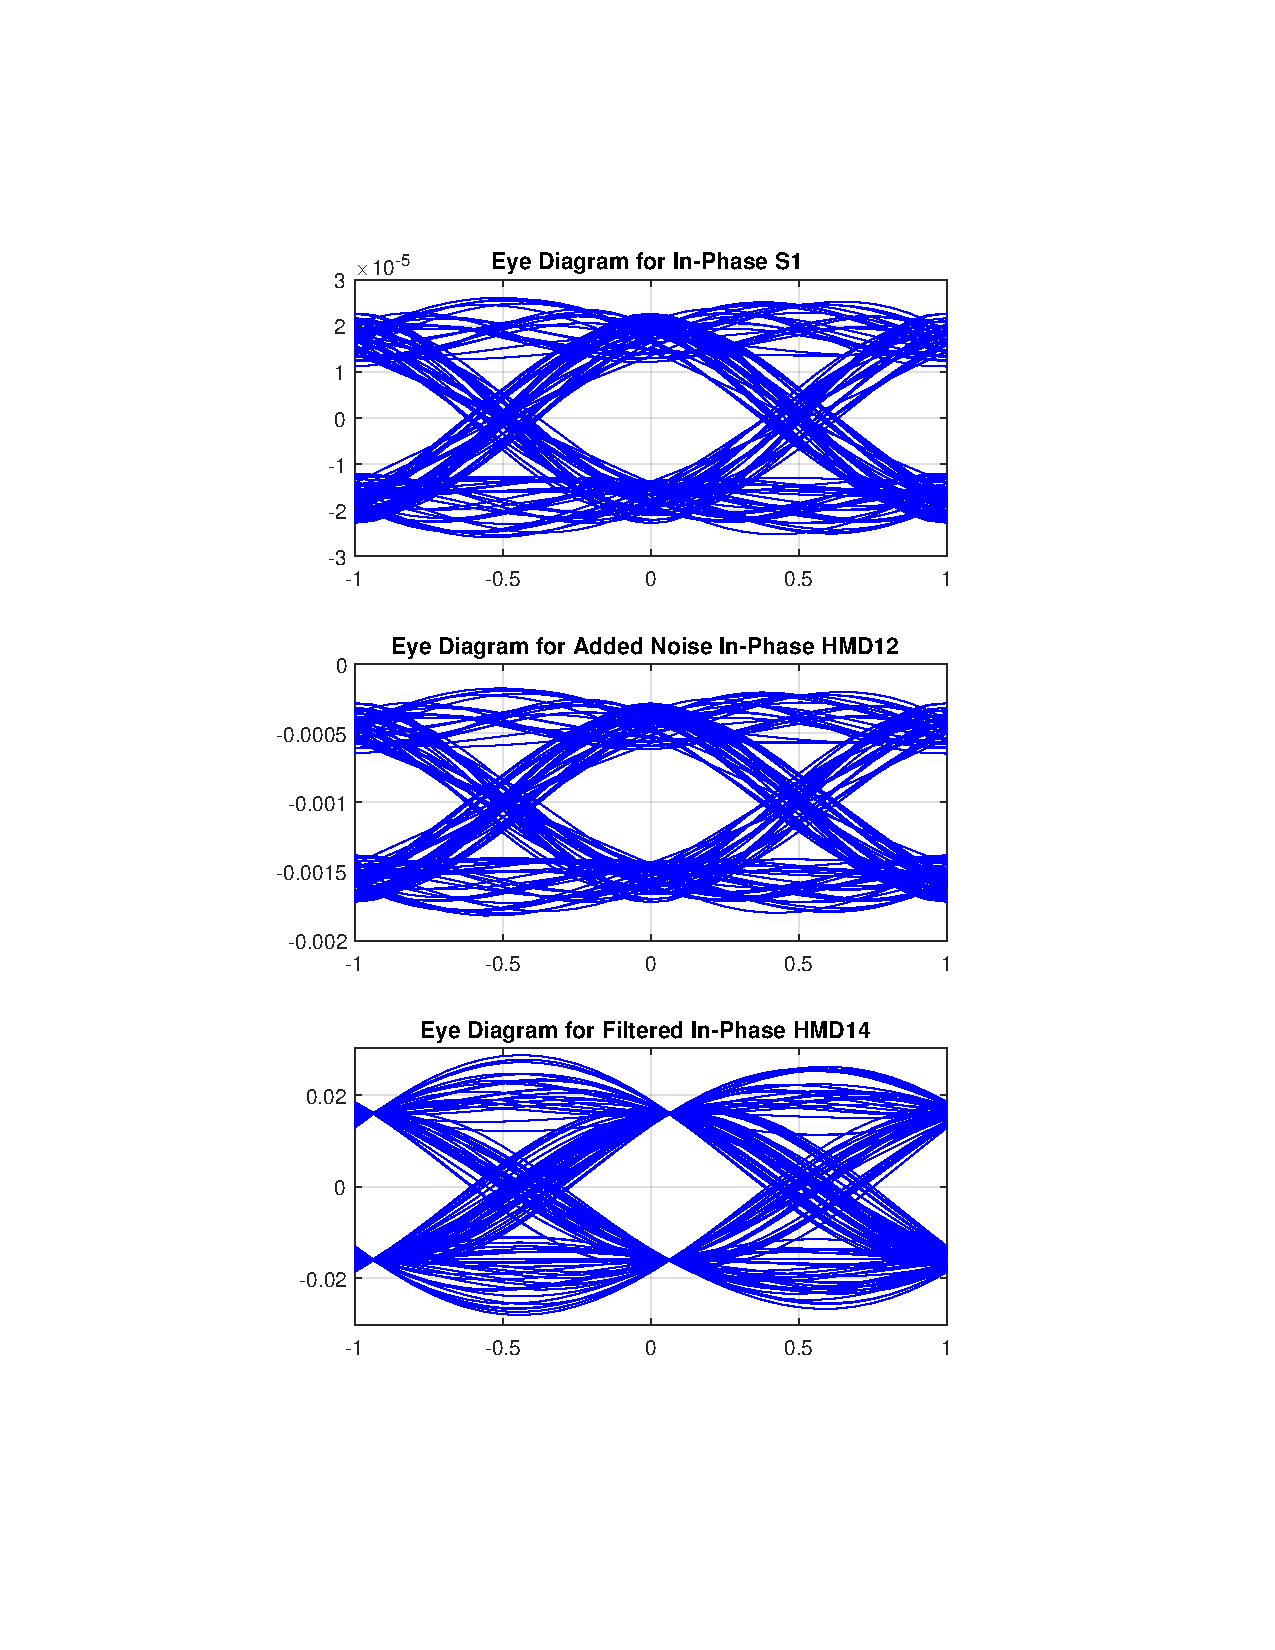
\includegraphics[clip, trim=5cm 4cm 5cm 4cm,
			width=\textwidth]{./sdf/m_qam_system/figures/eyes/if_nn_p_60_03.pdf}
	\end{subfigure}
	\begin{subfigure}{.45\textwidth}
		\centering
		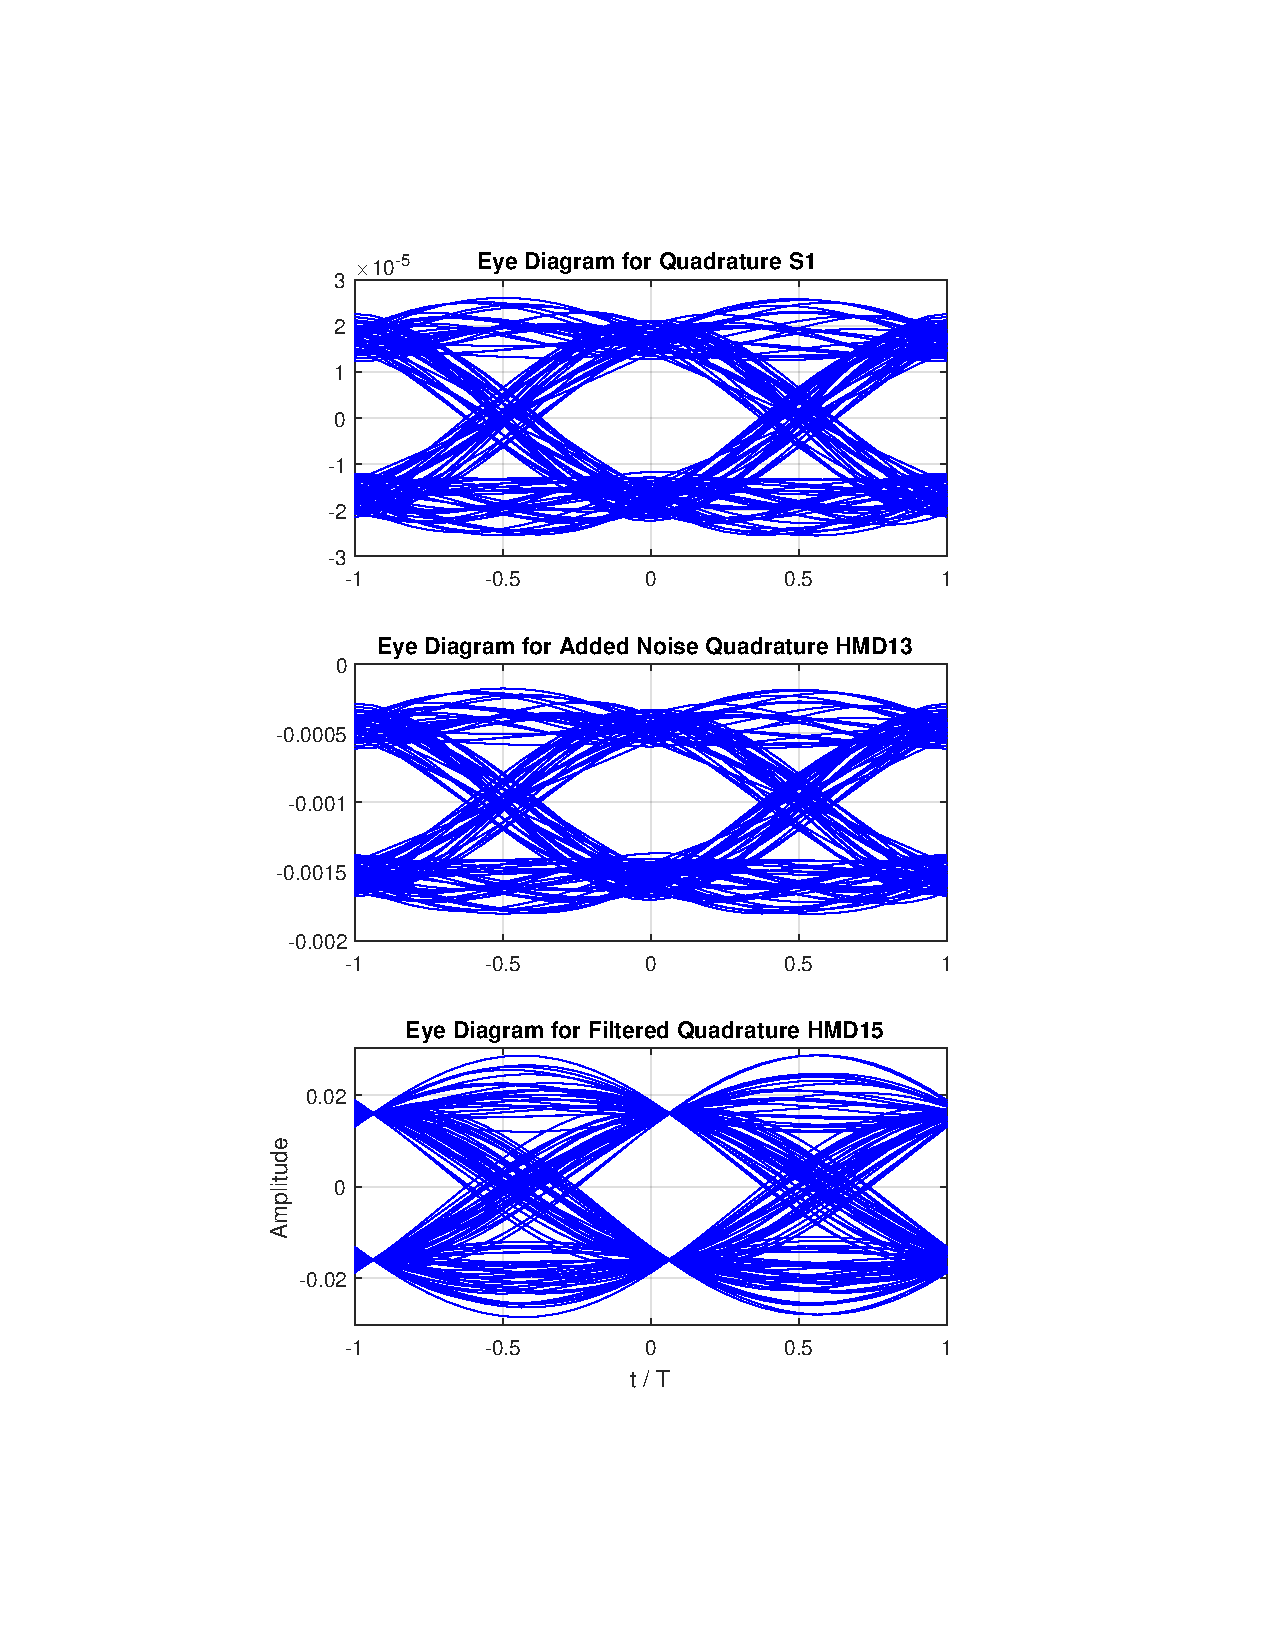
\includegraphics[clip, trim=5cm 4cm 5cm 4cm,
			width=\textwidth]{./sdf/m_qam_system/figures/eyes/q_nn_p_60_03.pdf}
	\end{subfigure}
	
	\caption{Eye diagrams using matched filtering with root-raised-cosine
		at three different points, without AWGN: the optical output signal S1 on the
		top; the amplified signal at the middle, HMD12 and HMD13 for both components;
		and after passing through the last root-raised-cosine filter, HMD14 and HMD15,
		for both components. Obtained through simulation with an optical power output
		of -60 dBm, 0 dBm at the local oscillator, a gain of $10^3$ at the amplifier,
		and a rolloff factor of 0.3.\label{fig:eyes_nn_rrc_03}}
	
\end{figure}

Thus, it can be concluded that, in order to avoid inter-symbol interference,
the filters used should be raised-cosine or root-raised-cosine, if not using a
filter at the receiver or if using matched filtering, respectively. As such,
from now on only these configurations will be used.

\subsubsection*{Signals with AWGN and high SNR}

In this section and the following one, a comparison will be presented between
not using a filter on the receiver and using matched filtering. This comparison
will be made for signals affected by added white gaussian noise, where the
noise is added to the signal after the amplifier stage and before the signal
passes through the filter on the receiver.

For the first case, where no filter is present at the receiver, a
raised-cosine filter will be used at the pulse shaper. For matched filtering, a
root-raised-cosine filter will be used at the pulse-shaper and the receiver.

Figures \ref{fig:eyes_n_rc_45_09}-\ref{fig:eyes_n_rrc_45_09} show the eye
diagrams for both these cases. The optical power used was $-45 dBm$, the
noise spectral density was set at $10^6 W/Hz$, and the roll-off factor was set
to $0.9$ in both cases. In both cases, its is still possible to visibly see the
approximate shape of the signal after noise is added, even without matched
filtering. However, it can be seen that the output signal in the case with
matched filtering is much less affected by noise, as the root-raised-cosine at
the receiver is rather effective at filtering the noise.


\begin{figure}[H]
	\centering
	\begin{subfigure}{.45\textwidth}
		\centering
		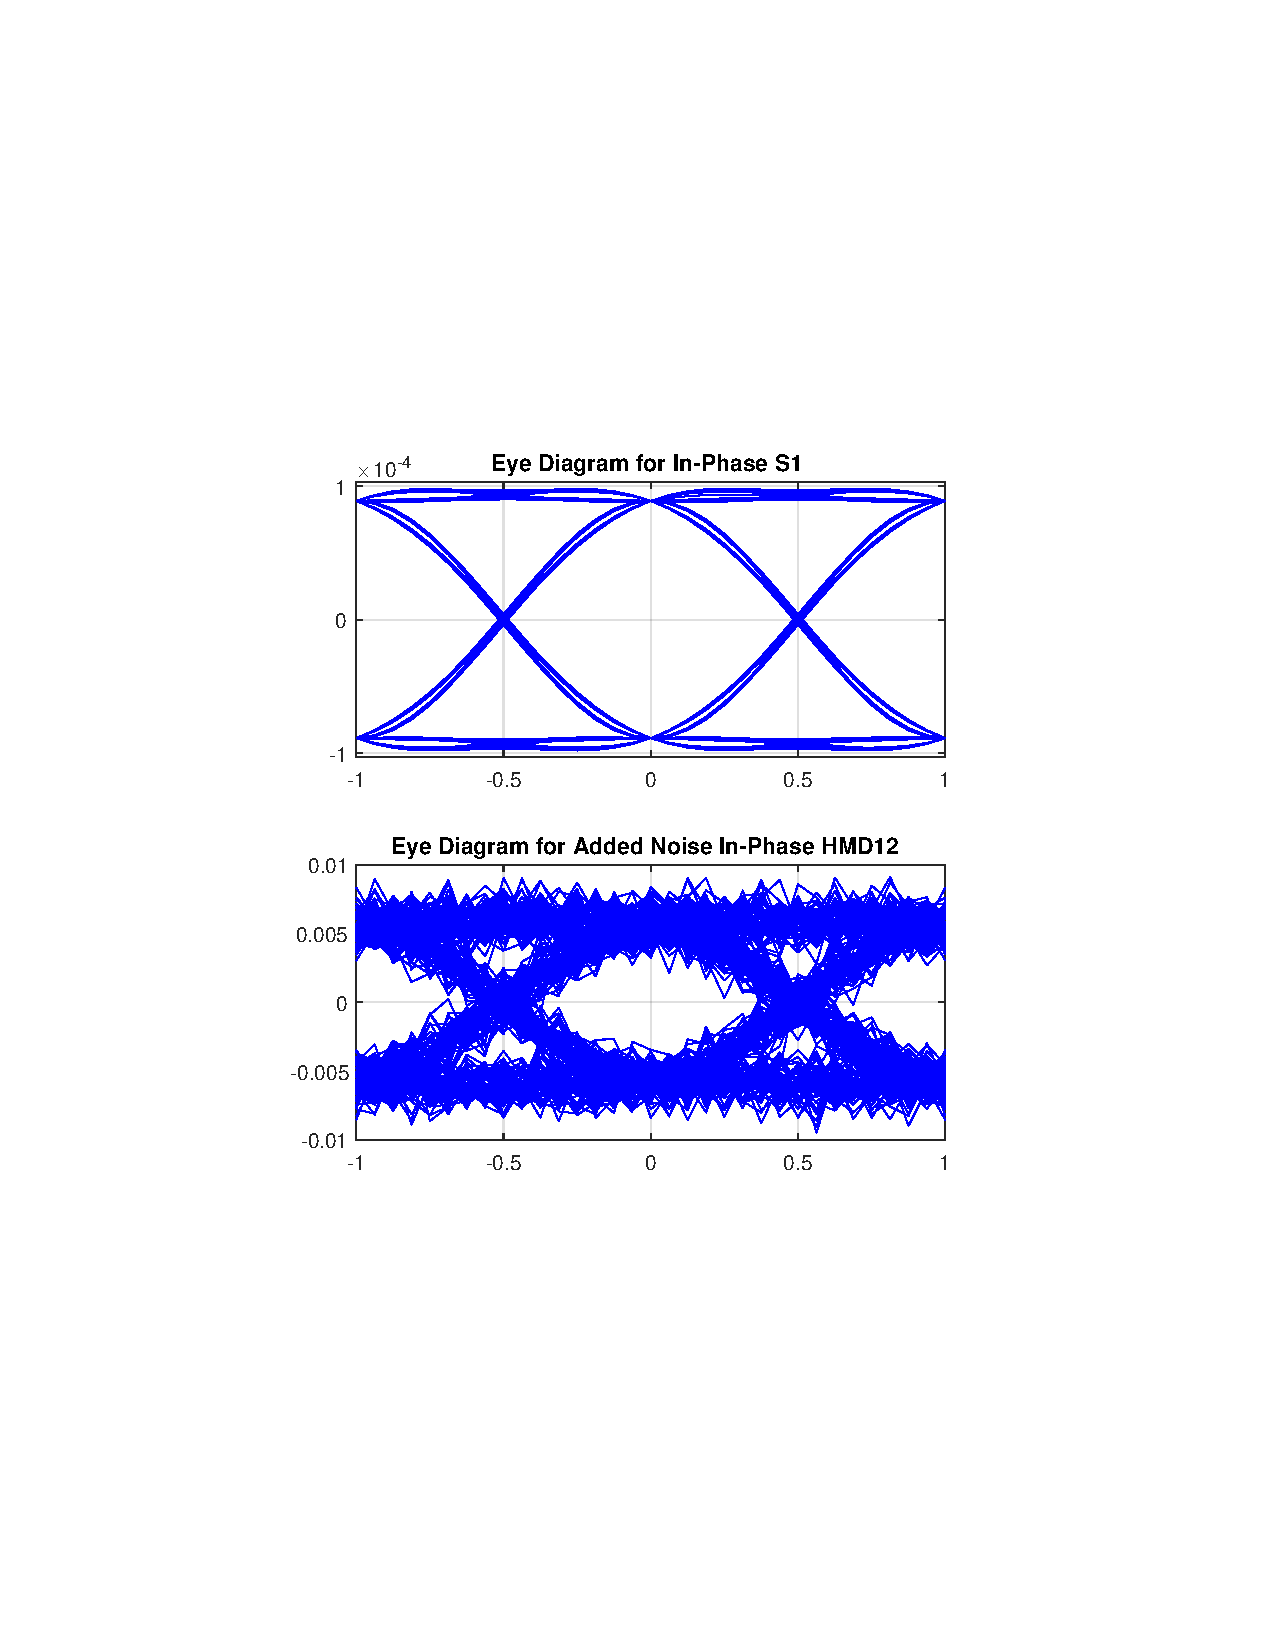
\includegraphics[clip, trim=5cm 4cm 5cm 4cm, width=\textwidth]{./sdf/m_qam_system/figures/eyes/if_n_nmf_45_60_rc_09.pdf}
	\end{subfigure}
	\begin{subfigure}{.45\textwidth}
		\centering
		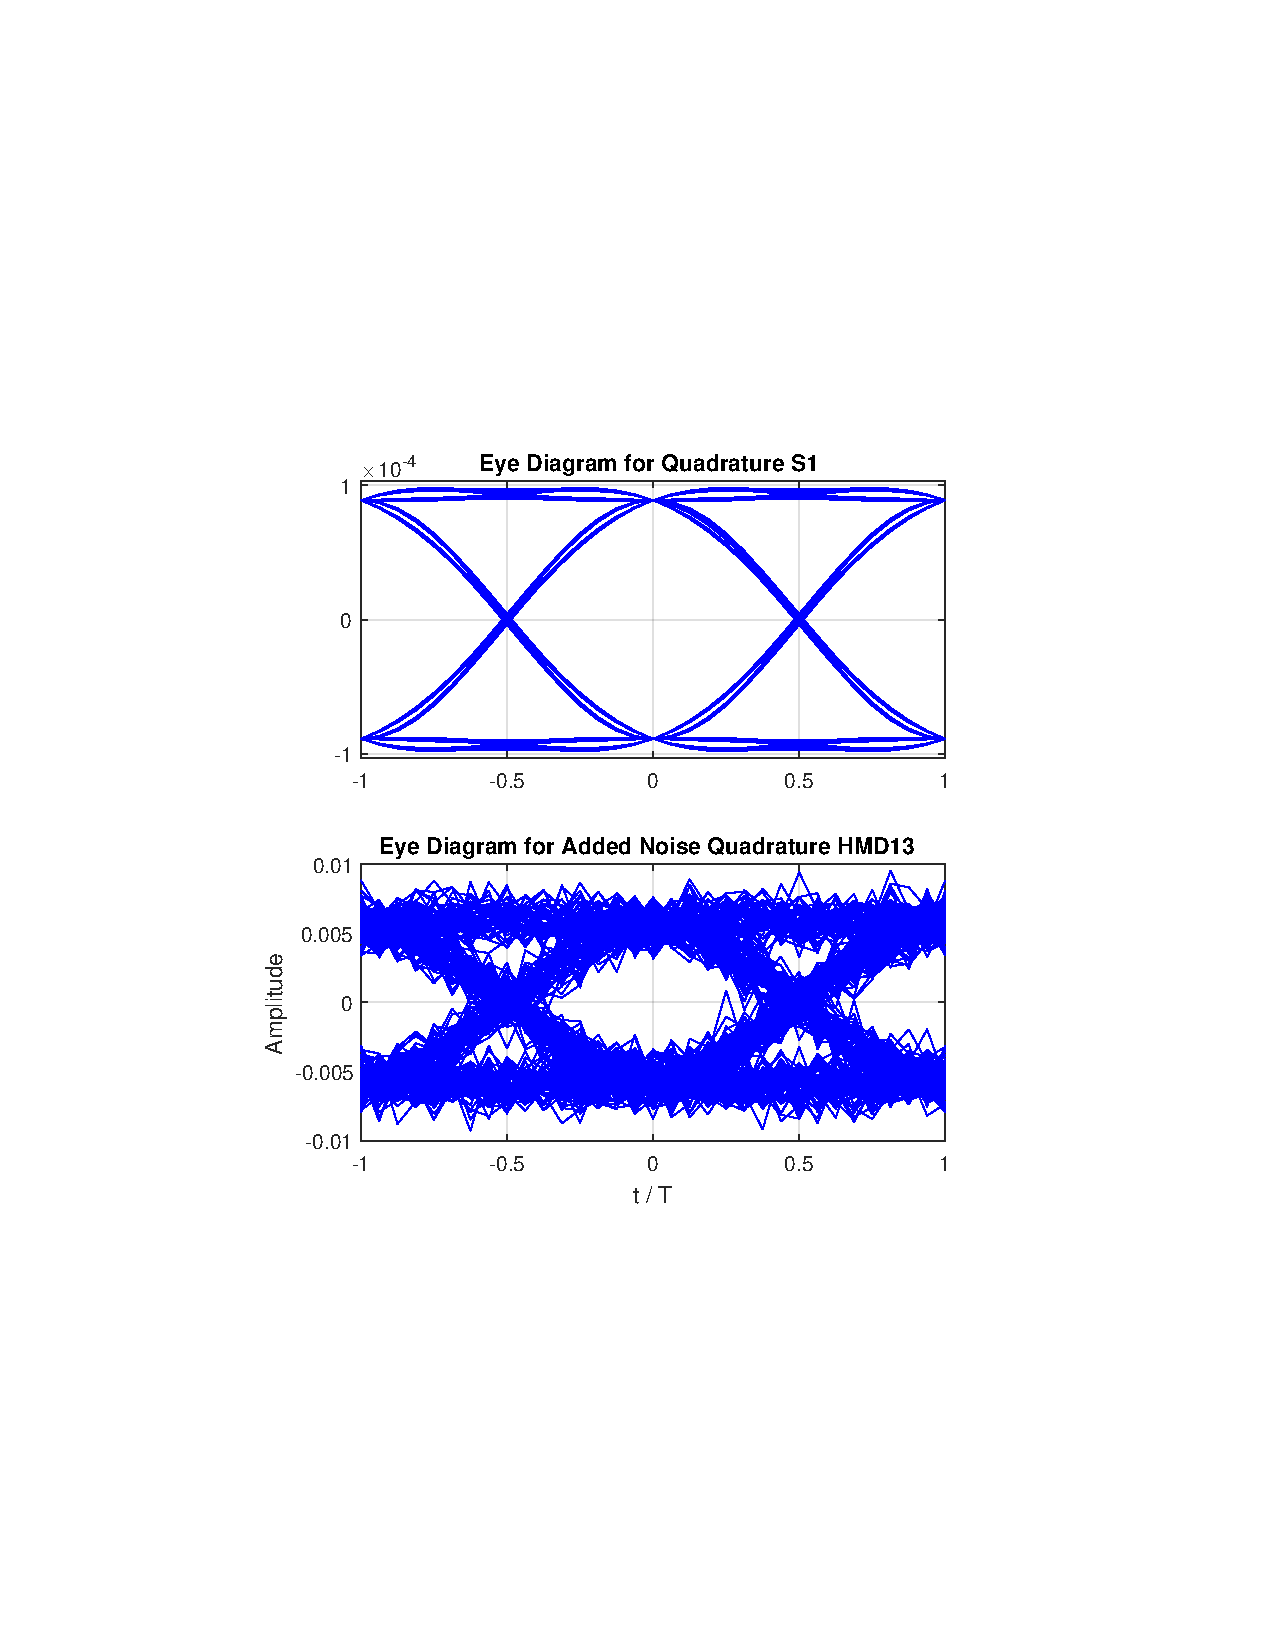
\includegraphics[clip, trim=5cm 4cm 5cm 4cm, width=\textwidth]{./sdf/m_qam_system/figures/eyes/q_n_nmf_45_60_rc_09.pdf}
	\end{subfigure}
	
	\caption{Eye diagrams without matched filtering using raised-cosine, at
		two different points: the optical output signal S1 on the top and the amplified
		signal with added noise, HMD12 and HMD13 for both components.
		Obtained through simulation with an optical power output of
		-45 dBm, 0 dBm at the local oscillator, a gain of $10^3$ at the amplifier, a
		noise spectral density of $10^{-6}$ and a rolloff factor of
		0.9.\label{fig:eyes_n_rc_45_09}}
\end{figure}

\begin{figure}[H]
	\centering
	\begin{subfigure}{.45\textwidth}
		\centering
		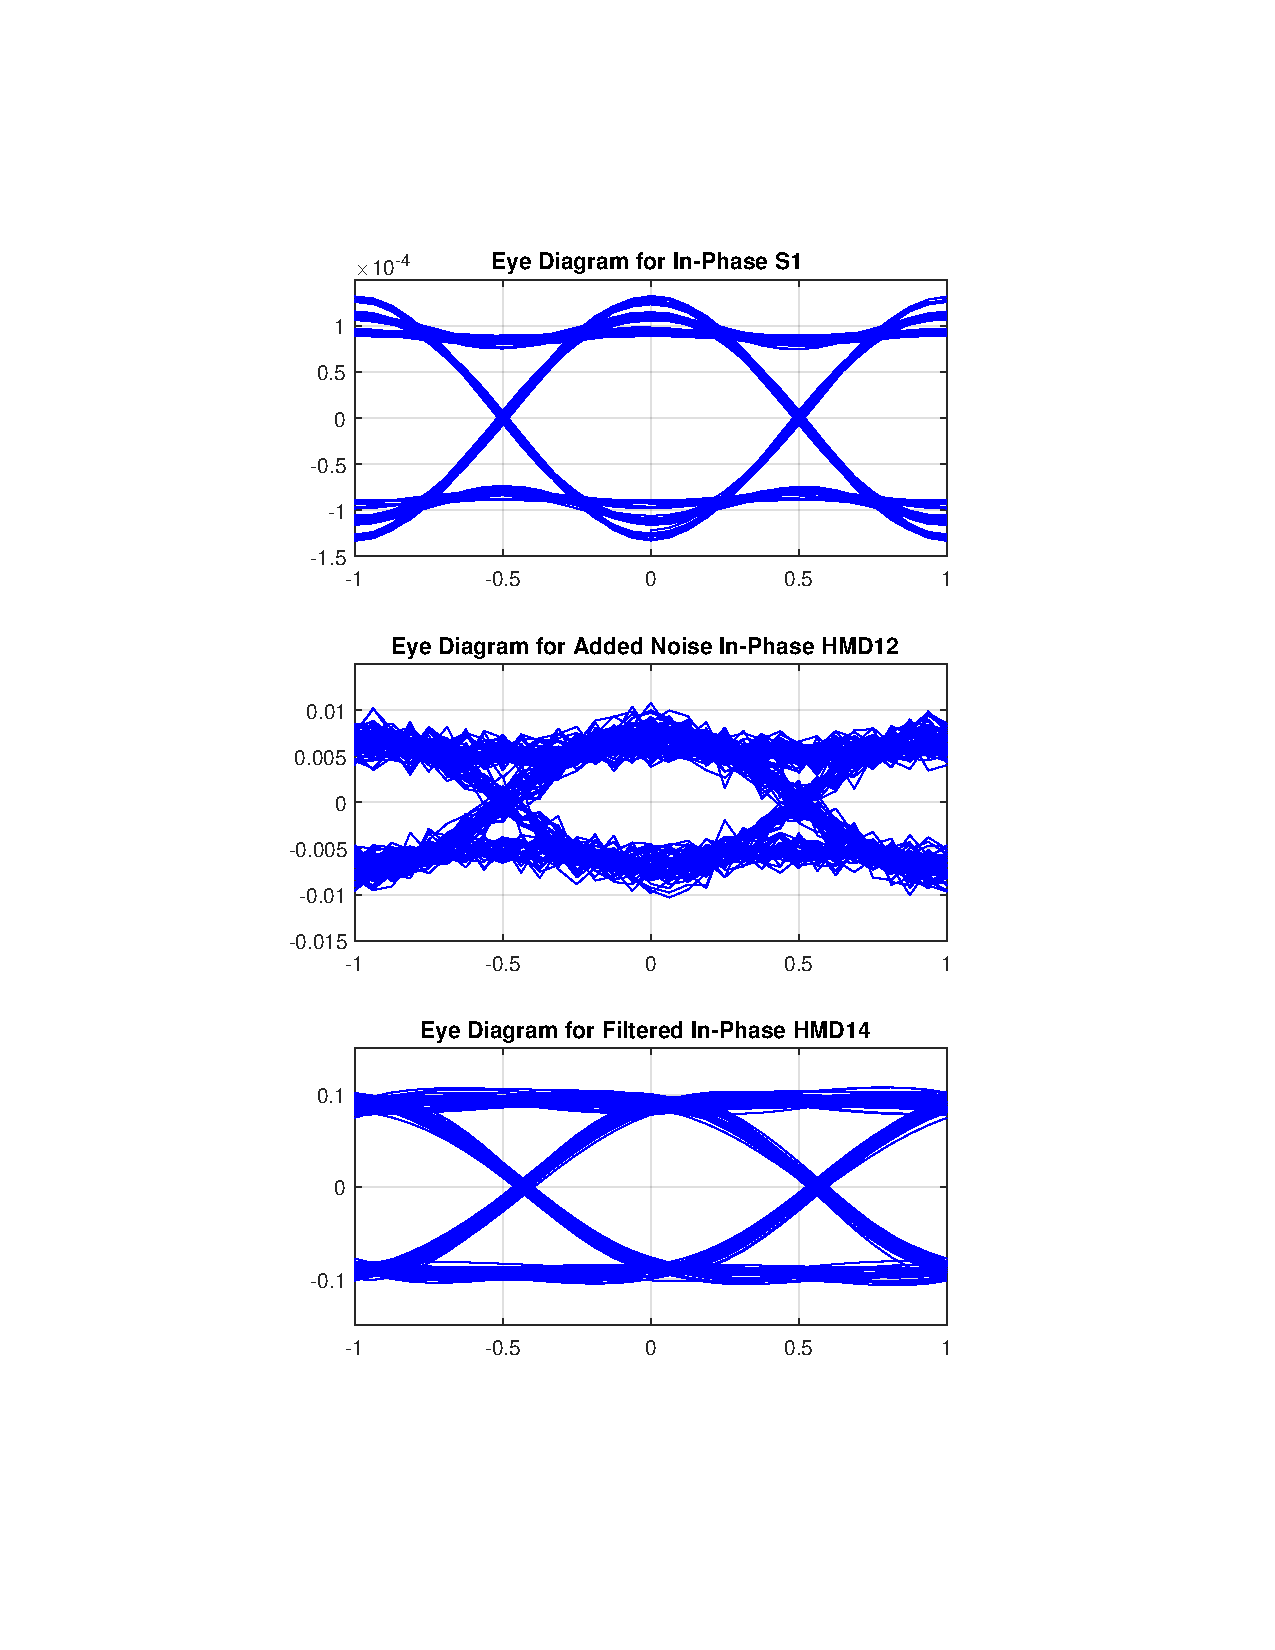
\includegraphics[clip, trim=5cm 4cm 5cm 4cm, width=\textwidth]{./sdf/m_qam_system/figures/eyes/if_p_45_09.pdf}
	\end{subfigure}
	\begin{subfigure}{.45\textwidth}
		\centering
		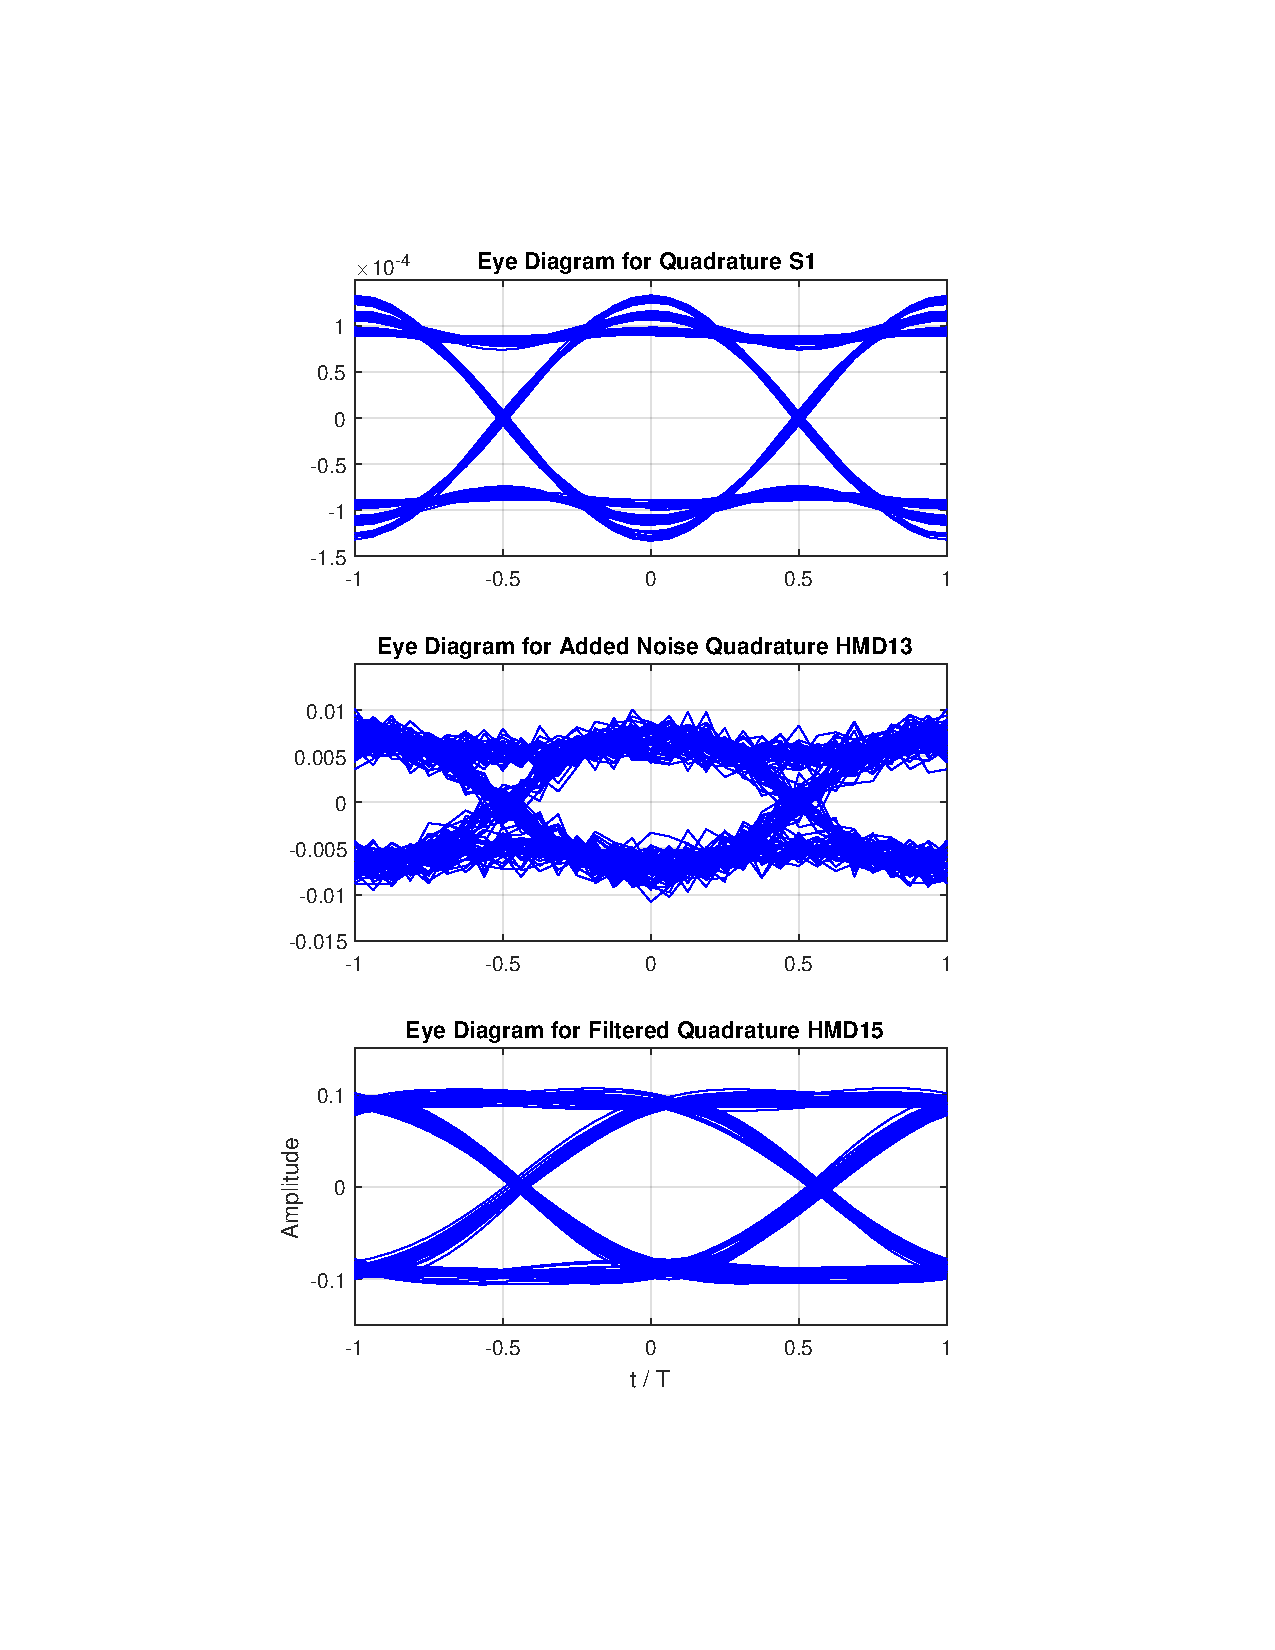
\includegraphics[clip, trim=5cm 4cm 5cm 4cm, width=\textwidth]{./sdf/m_qam_system/figures/eyes/q_p_45_09.pdf}
	\end{subfigure}
	
	\caption{Eye diagrams using matched filtering with root-raised-cosine
		at three different points: the optical output signal S1 on the top; the
		amplified signal with added noise at the middle, HMD12 and HMD13 for both
		components; and after passing through the last root-raised-cosine filter, HMD14
		and HMD15, for both components. Obtained through simulation with an optical
		power output of -45 dBm, 0 dBm at the local oscillator, a gain of $10^3$ at the
		amplifier, a noise spectral density of $10^{-6}$ and a rolloff factor of
		0.9.\label{fig:eyes_n_rrc_45_09}}
\end{figure}


Figures~\label{fig:eyes_n_rc_45_03} and~\label{fig:eyes_n_rrc_45_03} show the
cases described above, but with a roll-off factor of 0.3. It can be seen that
the case is in all aspects similar to the one presented above.


\begin{figure}[H]
	\centering
	\begin{subfigure}{.45\textwidth}
		\centering
		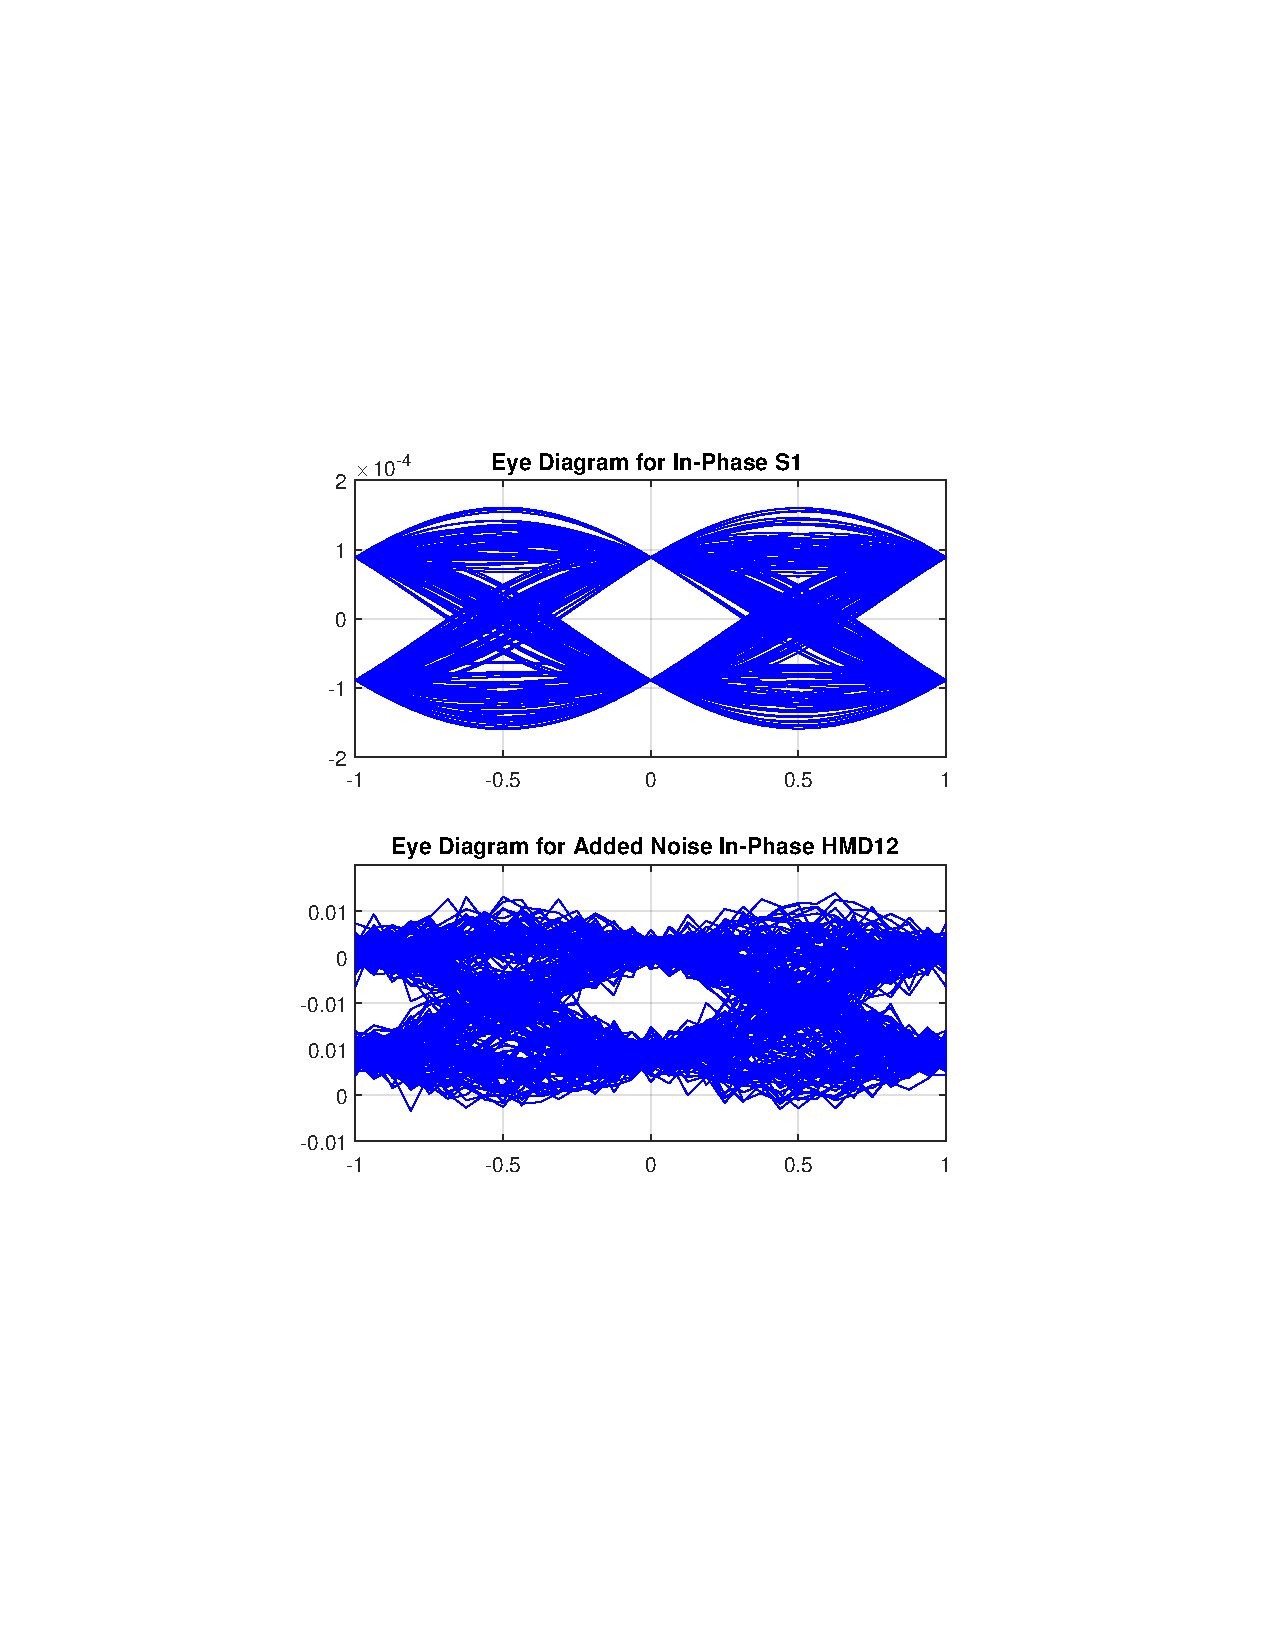
\includegraphics[clip, trim=5cm 4cm 5cm 4cm, width=\textwidth]{./sdf/m_qam_system/figures/eyes/if_n_nmf_45_60_rc.pdf}
	\end{subfigure}
	\begin{subfigure}{.45\textwidth}
		\centering
		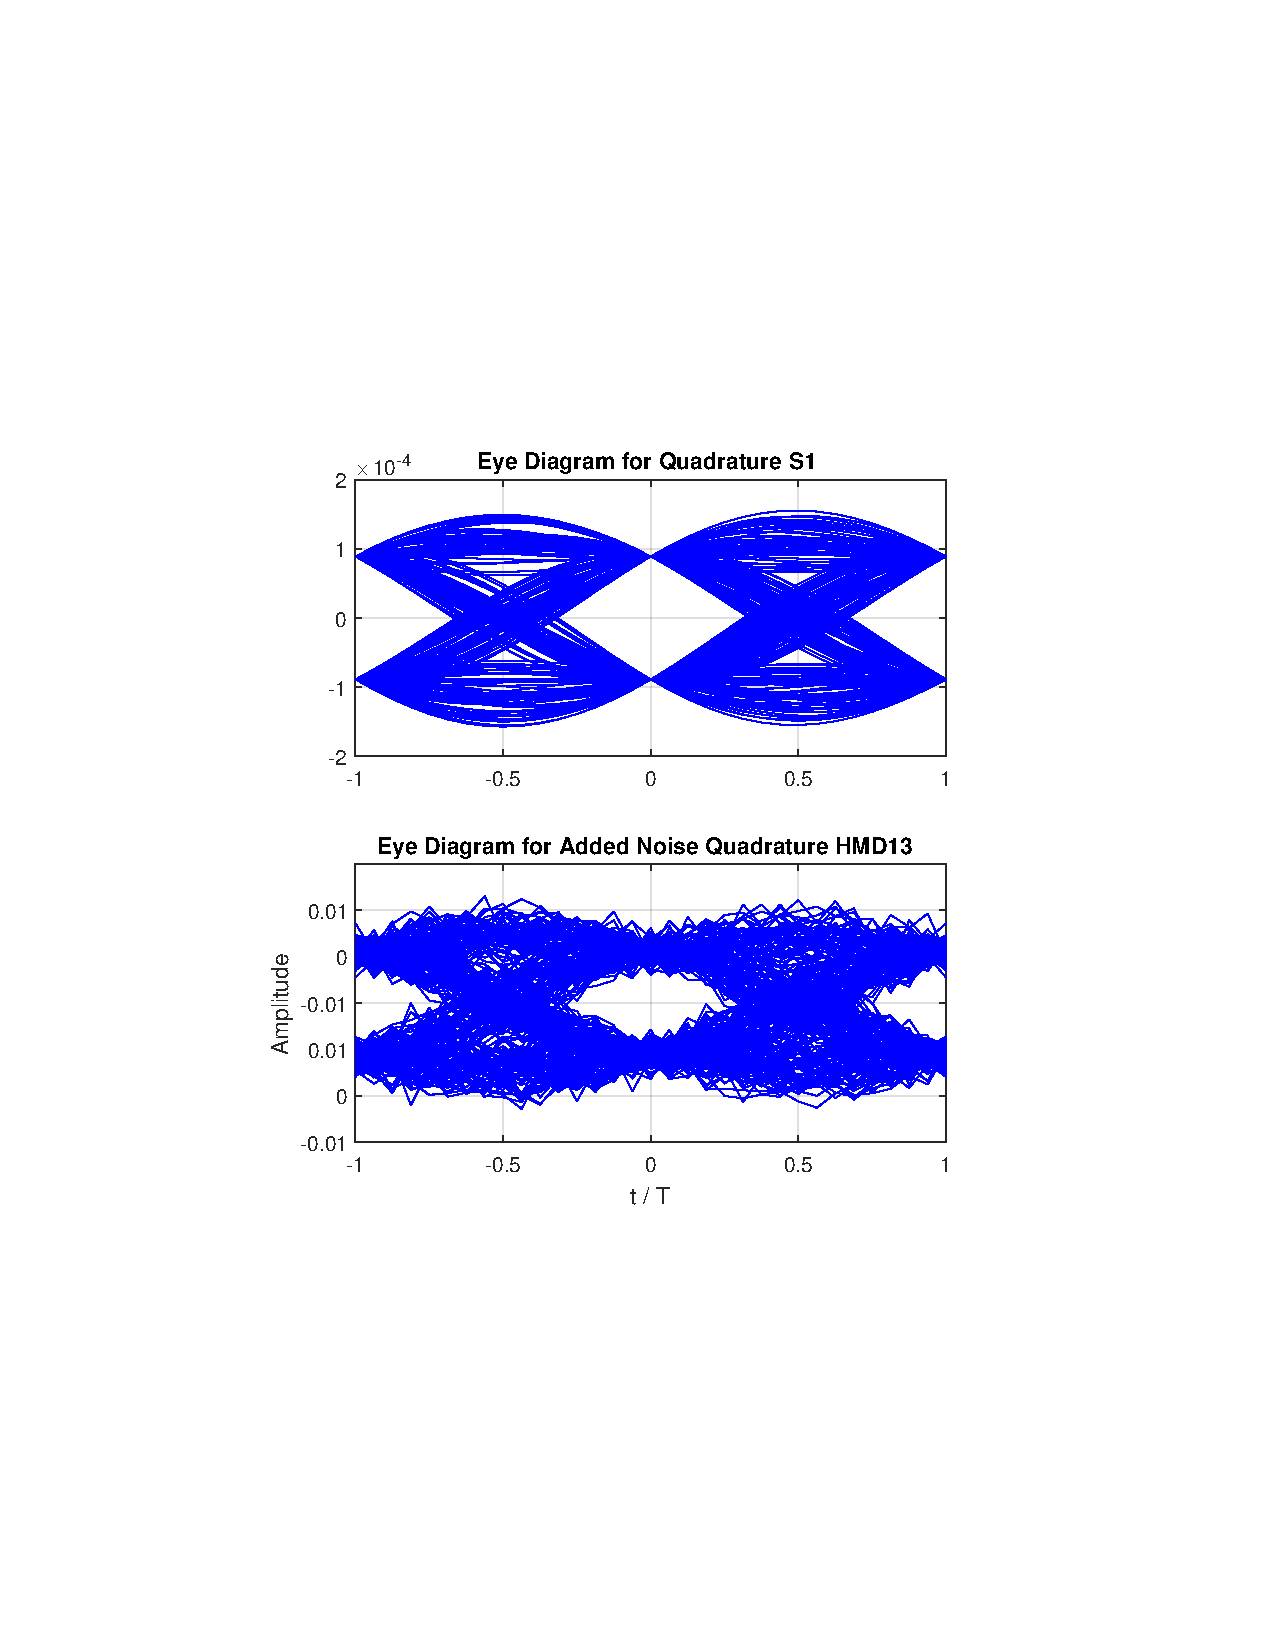
\includegraphics[clip, trim=5cm 4cm 5cm 4cm, width=\textwidth]{./sdf/m_qam_system/figures/eyes/q_n_nmf_45_60_rc.pdf}
	\end{subfigure}
	
	\caption{Eye diagrams without matched filtering with raised-cosine at
		two different points: the optical output signal S1 on the top and the amplified
		signal with added noise at the middle, HMD12 and HMD13, for
		both components. Obtained through simulation with an optical power output of
		-45 dBm, 0 dBm at the local oscillator, a gain of $10^3$ at the amplifier, a
		noise spectral density of $10^{-6}$ and a rolloff factor of
		0.3.\label{fig:eyes_n_rc_45_03}}
\end{figure}

\begin{figure}[H]
	\centering
	\begin{subfigure}{.45\textwidth}
		\centering
		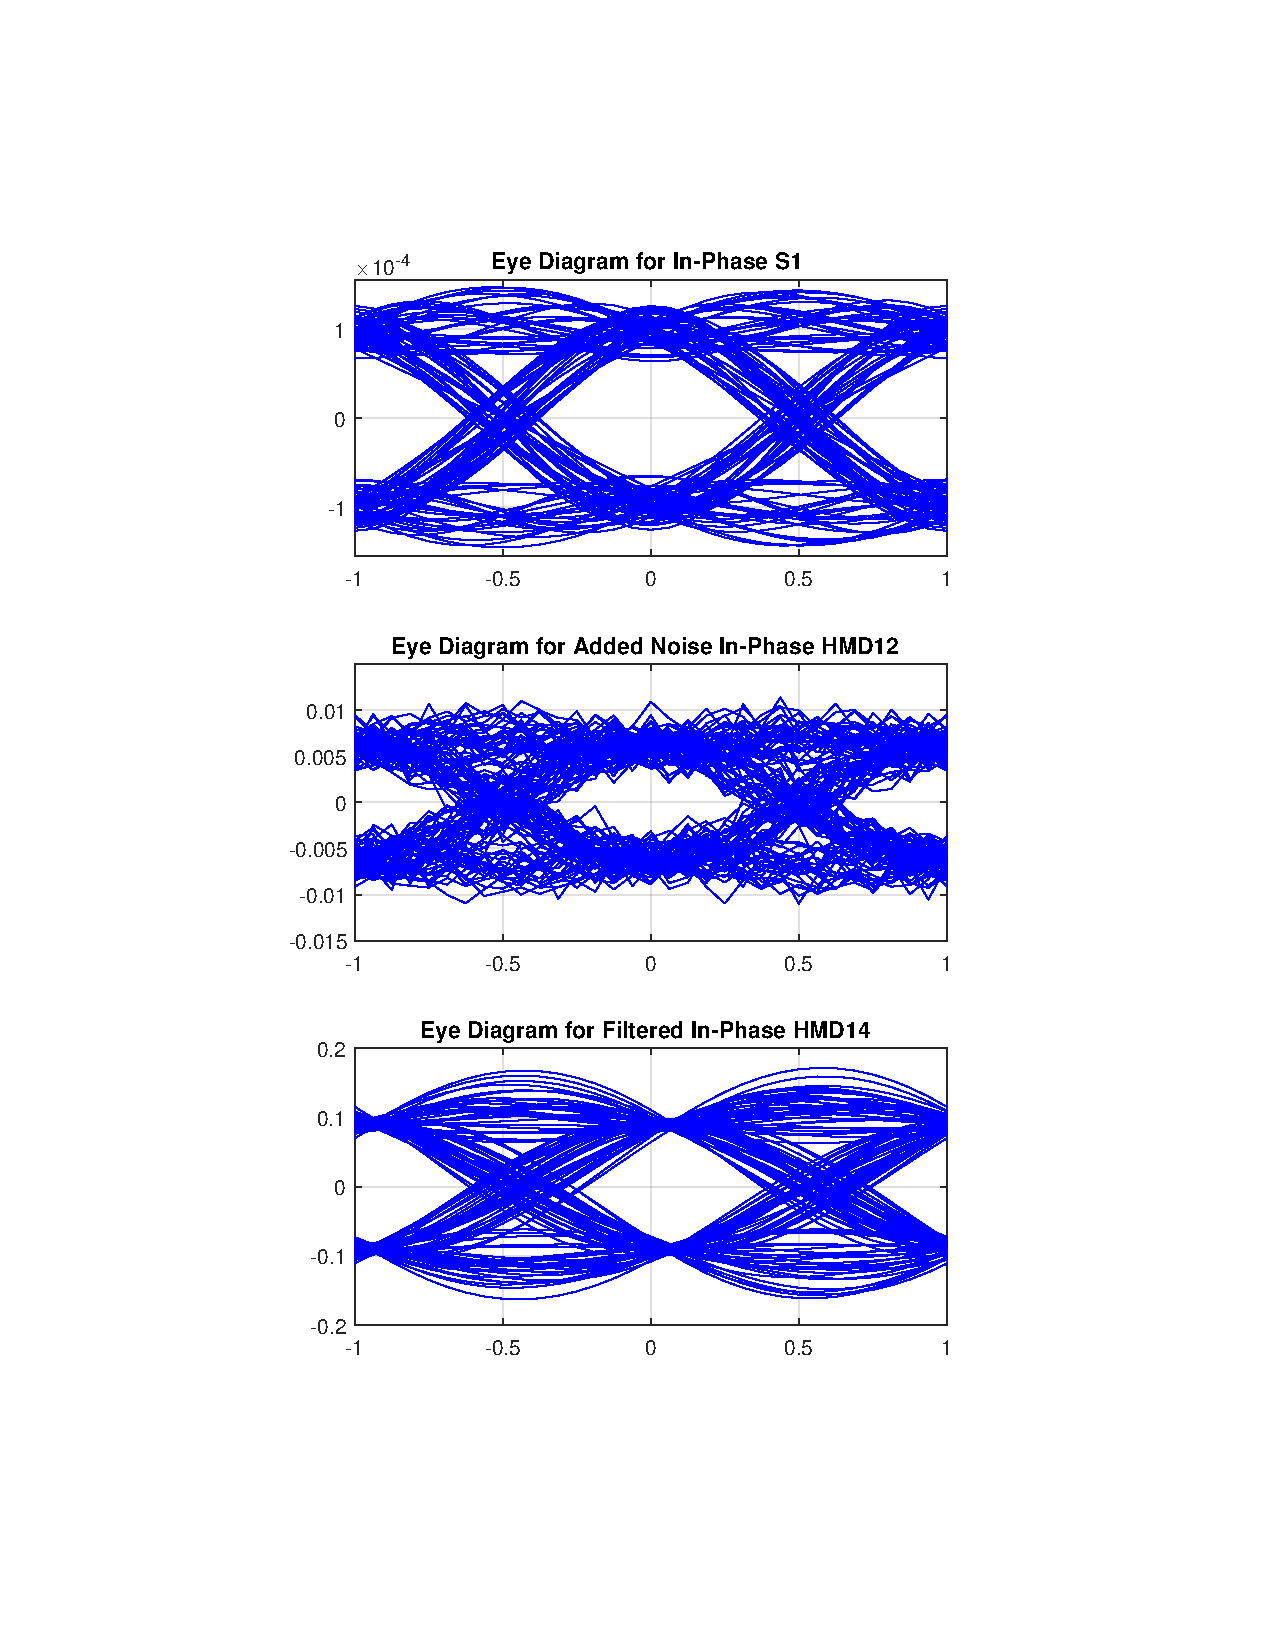
\includegraphics[clip, trim=5cm 4cm 5cm 4cm, width=\textwidth]{./sdf/m_qam_system/figures/eyes/if_p_45_03.pdf}
	\end{subfigure}
	\begin{subfigure}{.45\textwidth}
		\centering
		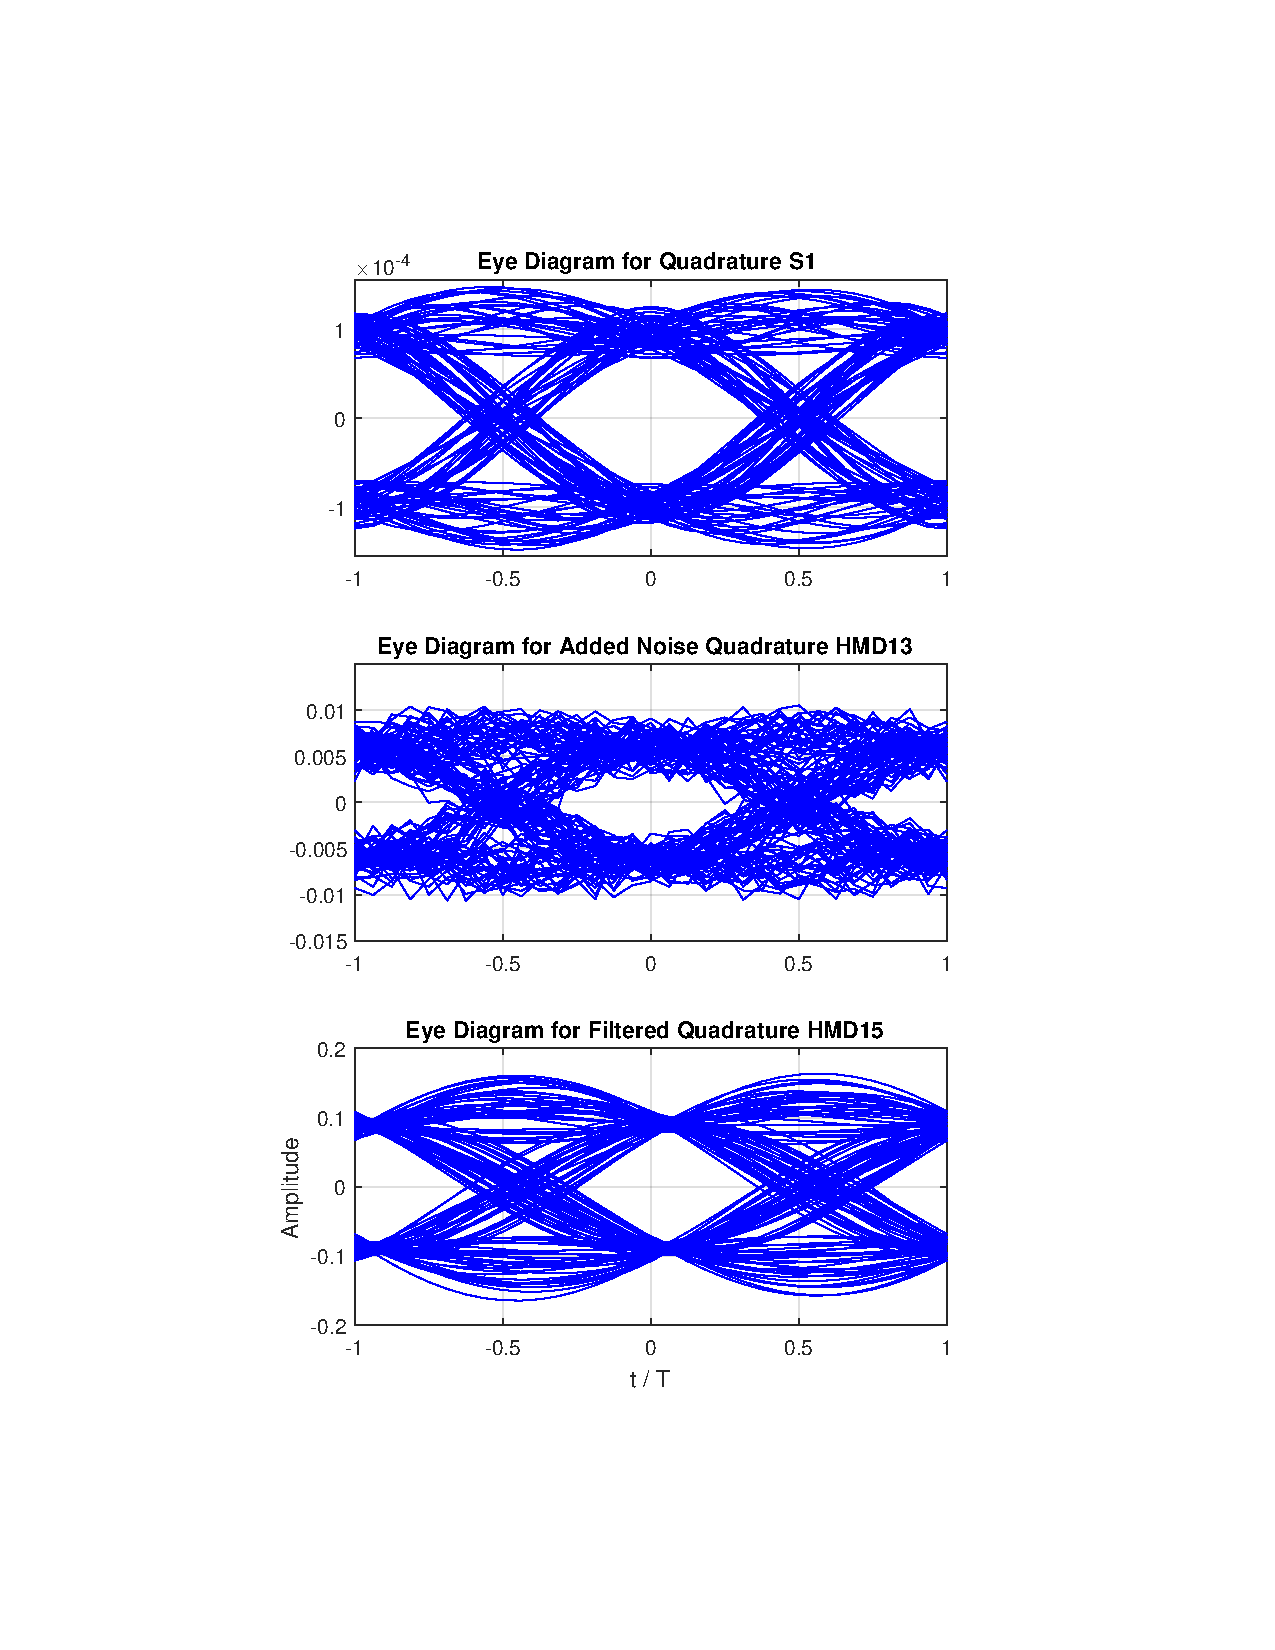
\includegraphics[clip, trim=5cm 4cm 5cm 4cm, width=\textwidth]{./sdf/m_qam_system/figures/eyes/q_p_45_03.pdf}
	\end{subfigure}
	
	\caption{Eye diagrams using matched filtering with root-raised-cosine
		at three different points: the optical output signal S1 on the top; the
		amplified signal with added noise at the middle, HMD12 and HMD13 for both
		components; and after passing through the last root-raised-cosine filter, HMD14
		and HMD15, for both components. Obtained through simulation with an optical
		power output of -45 dBm, 0 dBm at the local oscillator, a gain of $10^3$ at the
		amplifier, a noise spectral density of $10^{-6}$ and a rolloff factor of
		0.3.\label{fig:eyes_n_rrc_45_03}}
	
\end{figure}



\subsubsection*{Signals with AWGN and low SNR}
Figures \ref{fig:eyes_n_rrc_60_03}-\ref{fig:eyes_n_rc_60_09} show eye
diagrams similar to the previous section, but with a lower optical power ($-60~dBm$),
comparable to the spectral density of the noise ($10^{-6}$).



Figures~\ref{fig:eyes_n_rc_60_09} and~\ref{fig:eyes_n_rrc_60_09} show the
diagrams obtained without matched filtering and with matched filtering,
respectively, both using a roll-off factor of 0.9.

In this example the effects of matched filtering is even more obvious, as
without it the signal visually appears to be random noise.

\begin{figure}[H]
	\centering
	\begin{subfigure}{.45\textwidth}
		\centering
		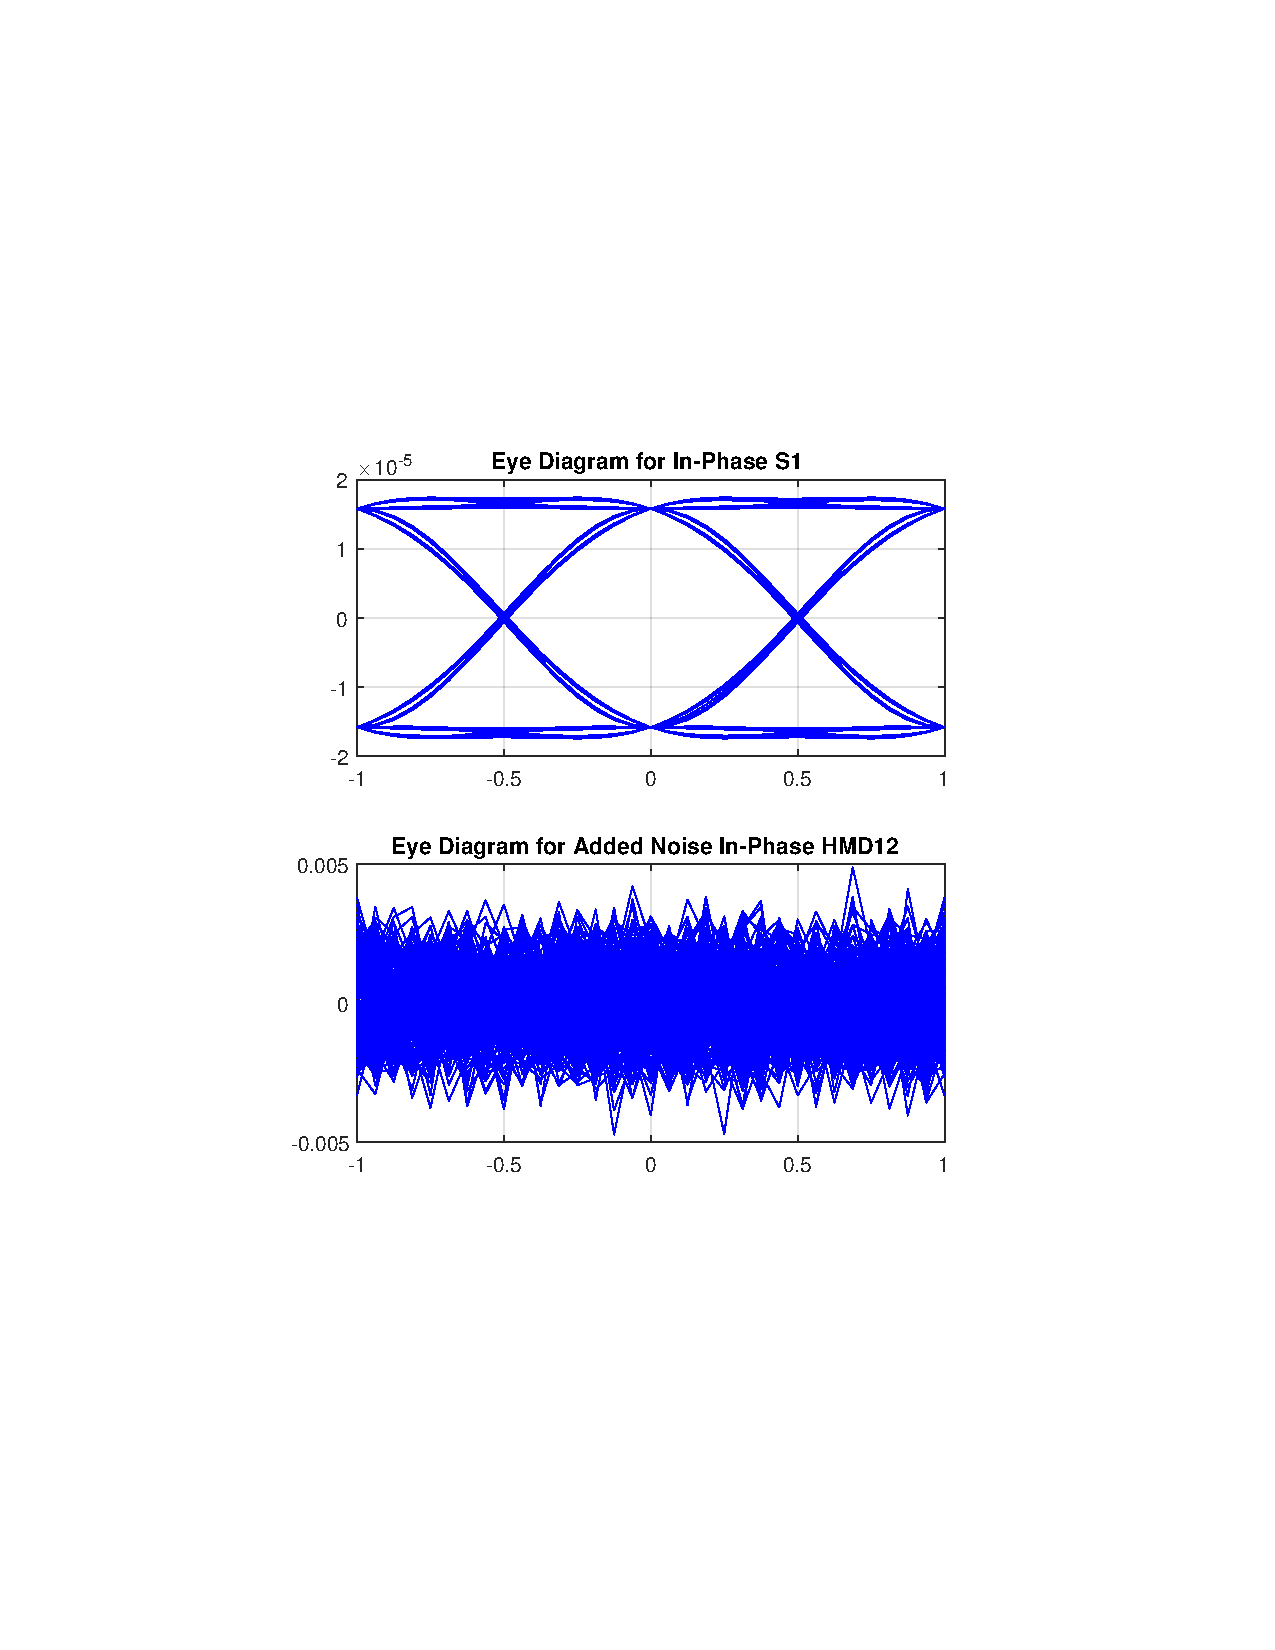
\includegraphics[clip, trim=5cm 4cm 5cm 4cm, width=\textwidth]{./sdf/m_qam_system/figures/eyes/if_n_nmf_60_60_rc_09.pdf}
	\end{subfigure}
	\begin{subfigure}{.45\textwidth}
		\centering
		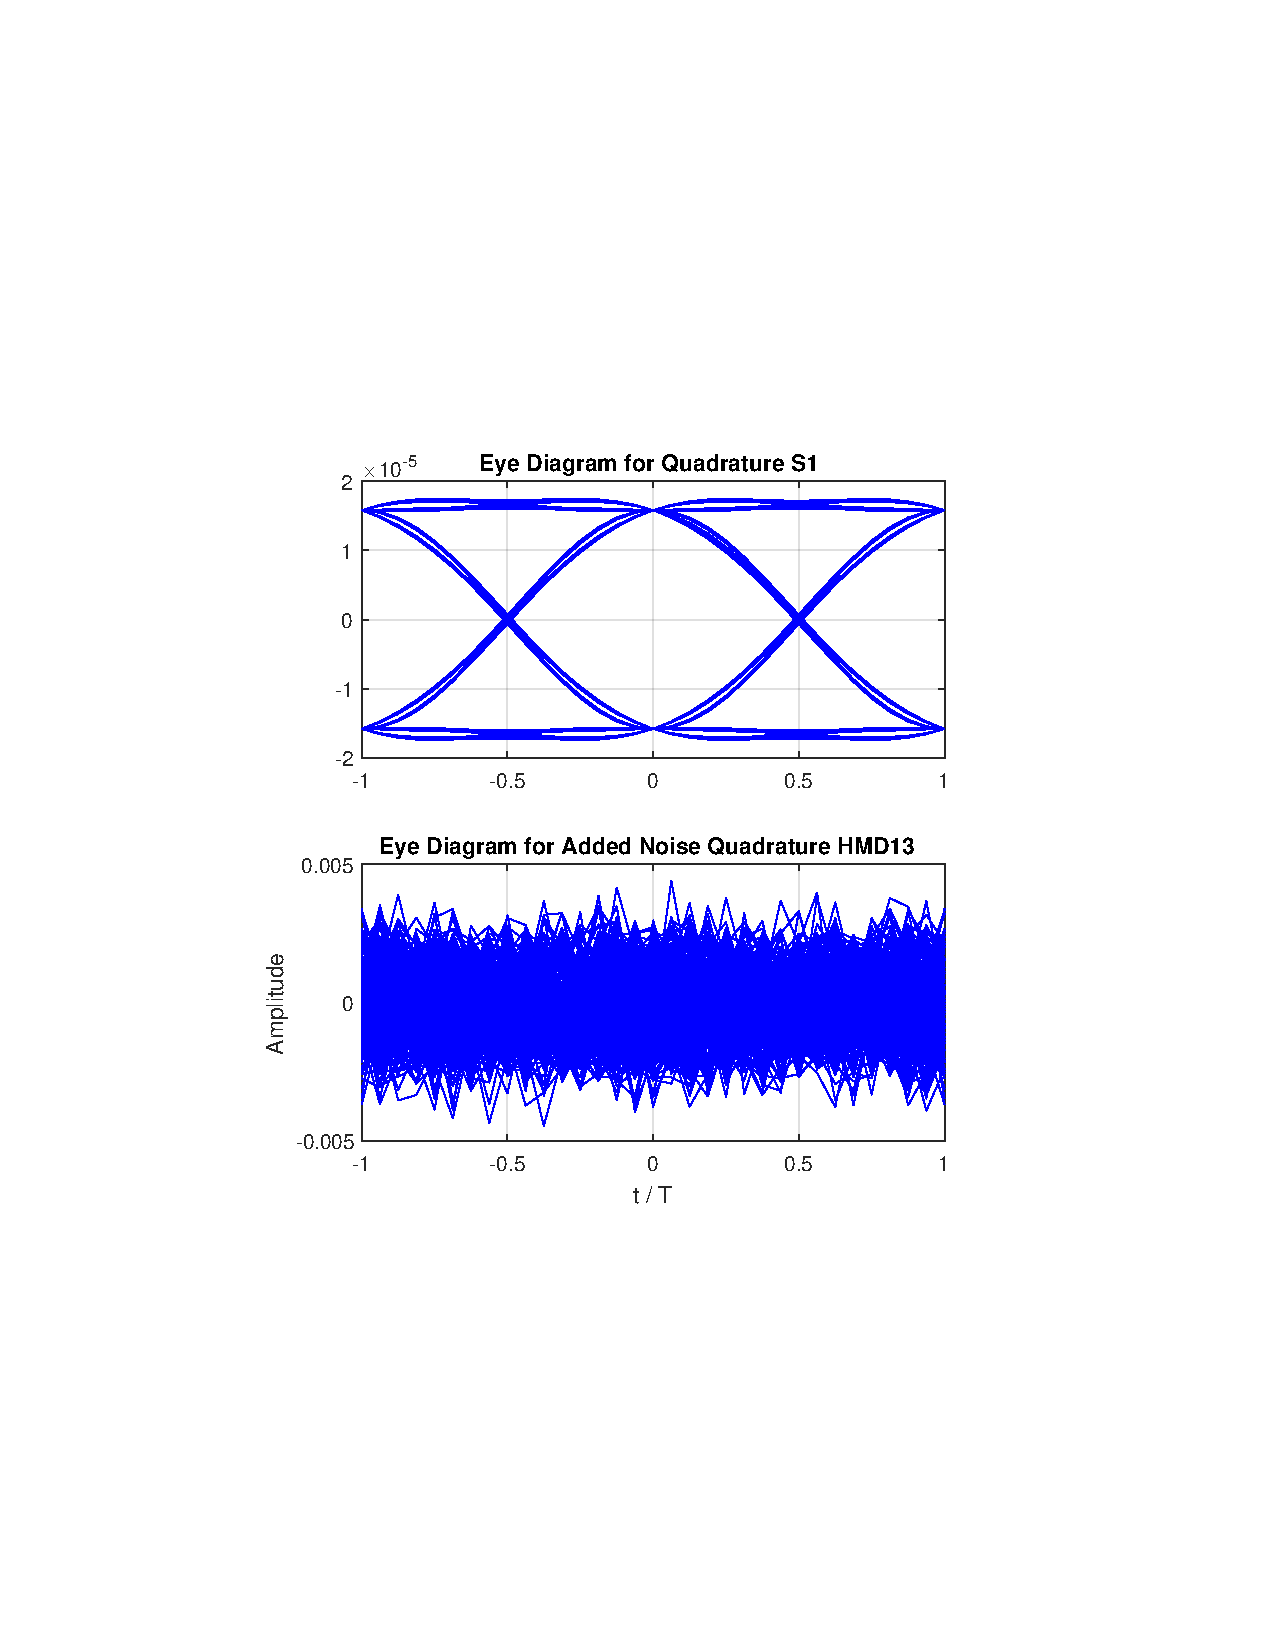
\includegraphics[clip, trim=5cm 4cm 5cm 4cm, width=\textwidth]{./sdf/m_qam_system/figures/eyes/q_n_nmf_60_60_rc_09.pdf}
	\end{subfigure}
	
	\caption{Eye diagrams without matched filtering with raised-cosine at
		two different points: the optical output signal S1 on the top and the amplified
		signal with added noise at the middle, HMD12 and HMD13 for both
		components. Obtained through simulation with an optical power output of -60
		dBm, 0 dBm at the local oscillator, a gain of $10^3$ at the amplifier, a noise
		spectral density of $10^{-6}$ and a rolloff factor of
		0.9.\label{fig:eyes_n_rc_60_09}}
\end{figure}


\begin{figure}[H]
	\centering
	\begin{subfigure}{.45\textwidth}
		\centering
		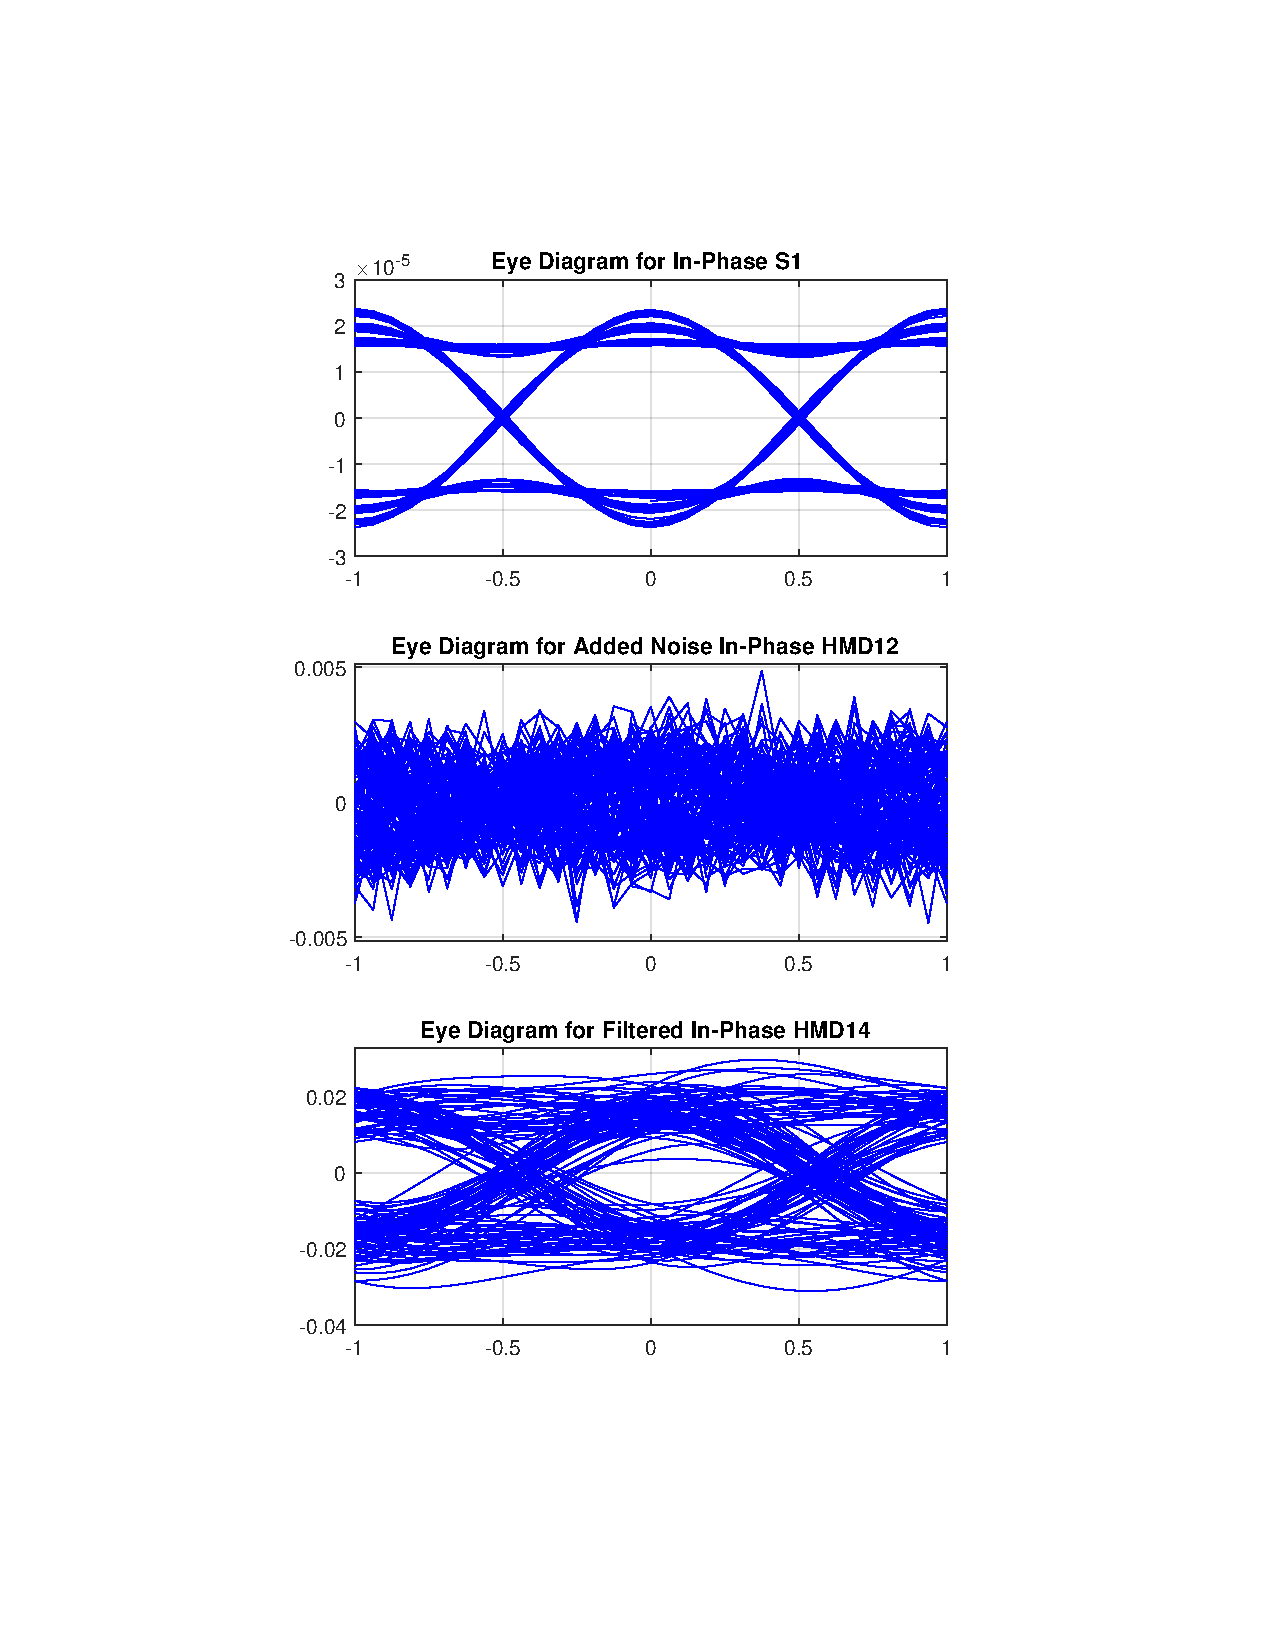
\includegraphics[clip, trim=5cm 4cm 5cm 4cm, width=\textwidth]{./sdf/m_qam_system/figures/eyes/if_p_60_09.pdf}
	\end{subfigure}
	\begin{subfigure}{.45\textwidth}
		\centering
		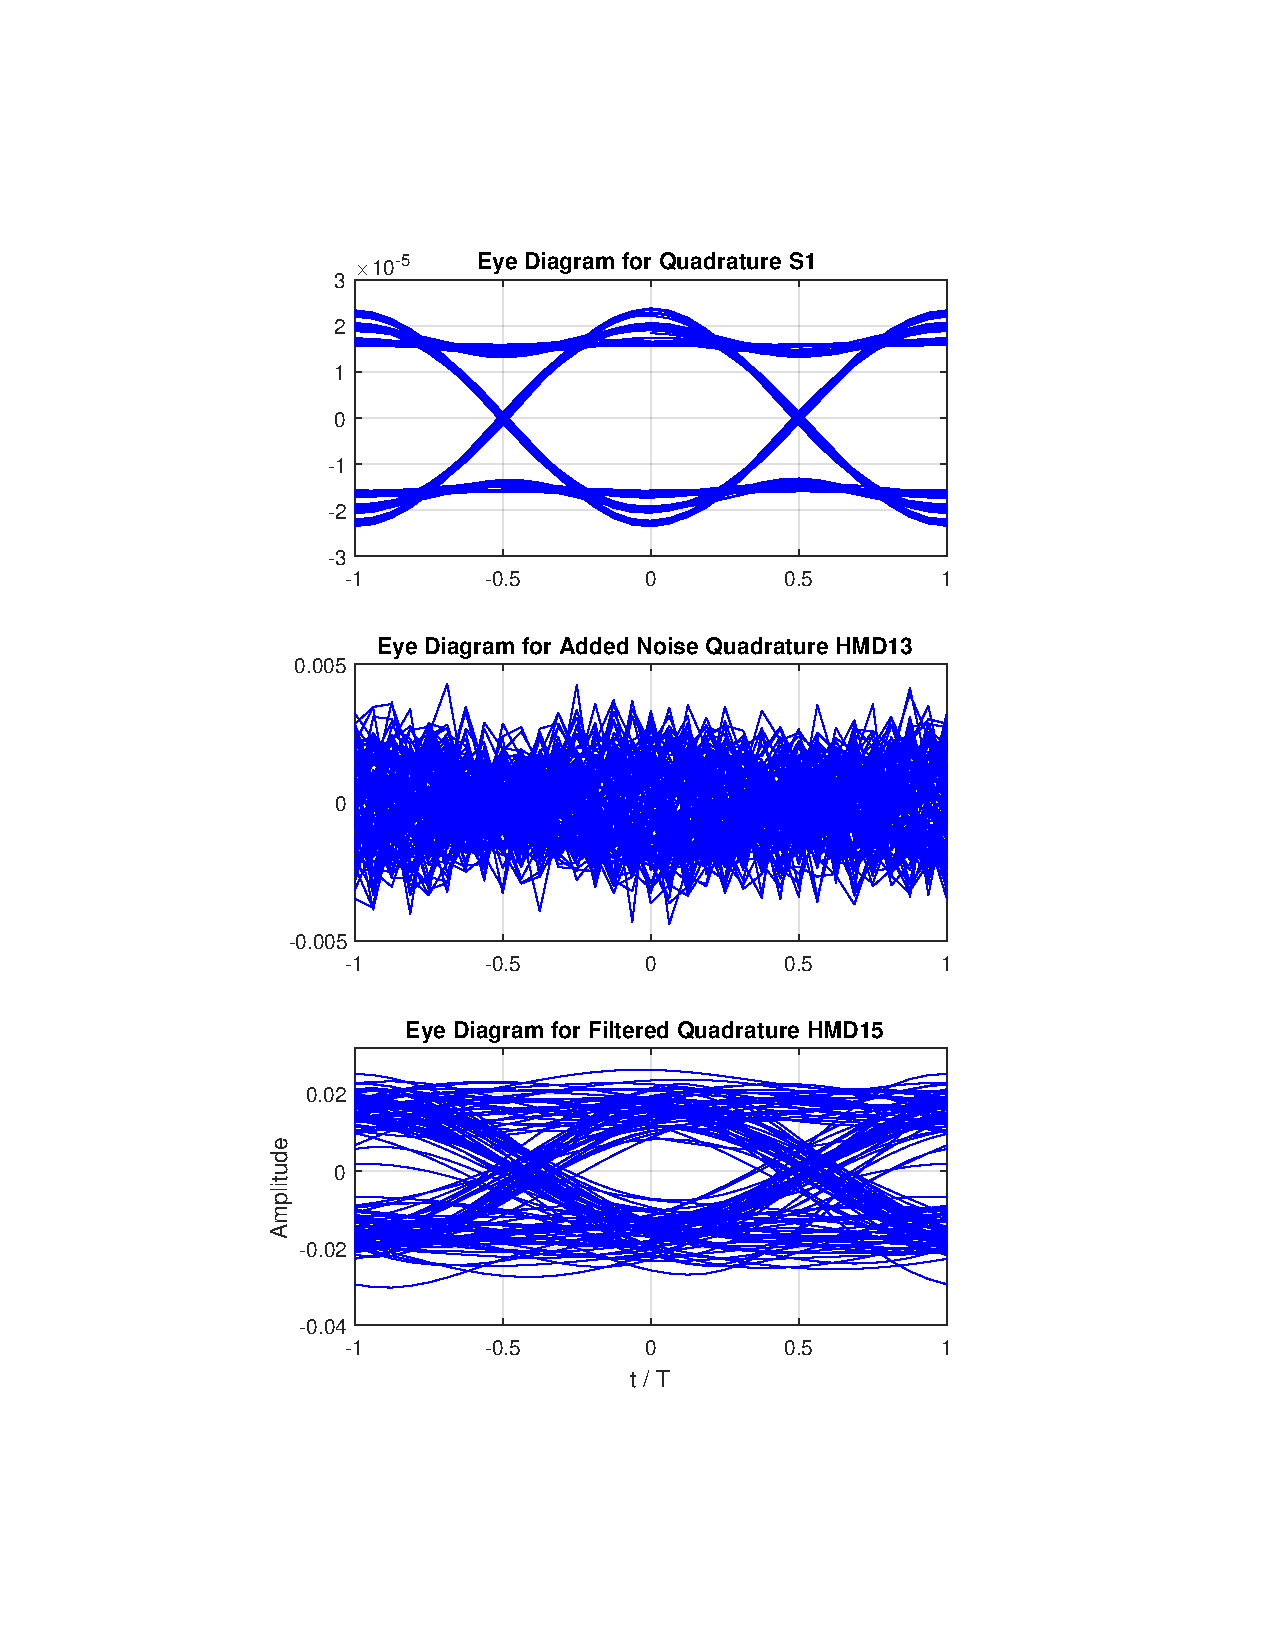
\includegraphics[clip, trim=5cm 4cm 5cm 4cm, width=\textwidth]{./sdf/m_qam_system/figures/eyes/q_p_60_09.pdf}
	\end{subfigure}
	
	\caption{Eye diagrams using matched filtering with root-raised-cosine at three different points: the optical output signal S1 on the top; the amplified signal with added noise at the middle, HMD12 and HMD13 for both components; and after passing through the last root-raised-cosine filter, HMD14 and HMD15, for both components. Obtained through simulation with an optical power output of -60 dBm, 0 dBm at the local oscillator, a gain of $10^3$ at the amplifier, a noise spectral density of $10^{-6}$ and a rolloff factor of 0.9.\label{fig:eyes_n_rrc_60_09}}
	
\end{figure}


Figures~\ref{fig:eyes_n_rc_60_03} and~\ref{fig:eyes_n_rrc_60_09} show the same
case but using a roll-off factor of 0.3.

\begin{figure}[H]
	\centering
	\begin{subfigure}{.45\textwidth}
		\centering
		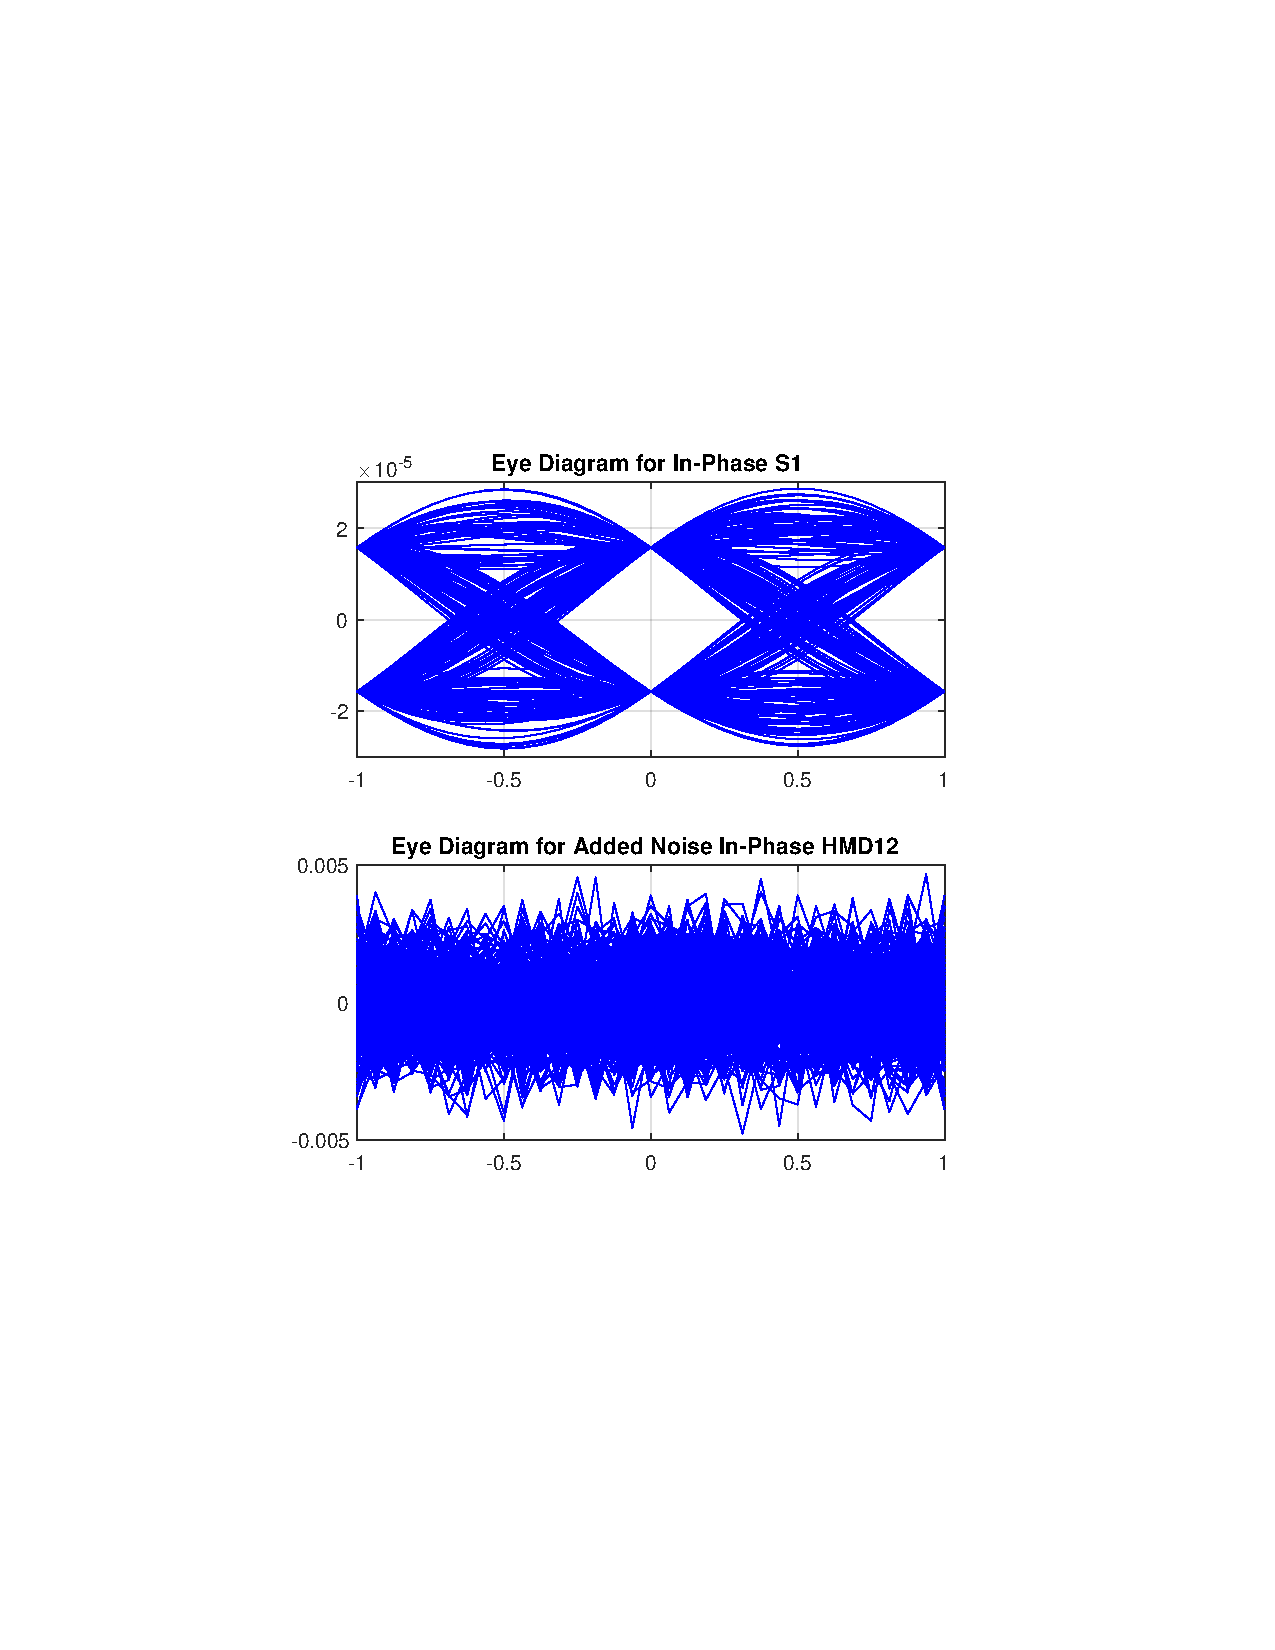
\includegraphics[clip, trim=5cm 4cm 5cm 4cm, width=\textwidth]{./sdf/m_qam_system/figures/eyes/if_n_nmf_60_60_rc_03.pdf}
	\end{subfigure}
	\begin{subfigure}{.45\textwidth}
		\centering
		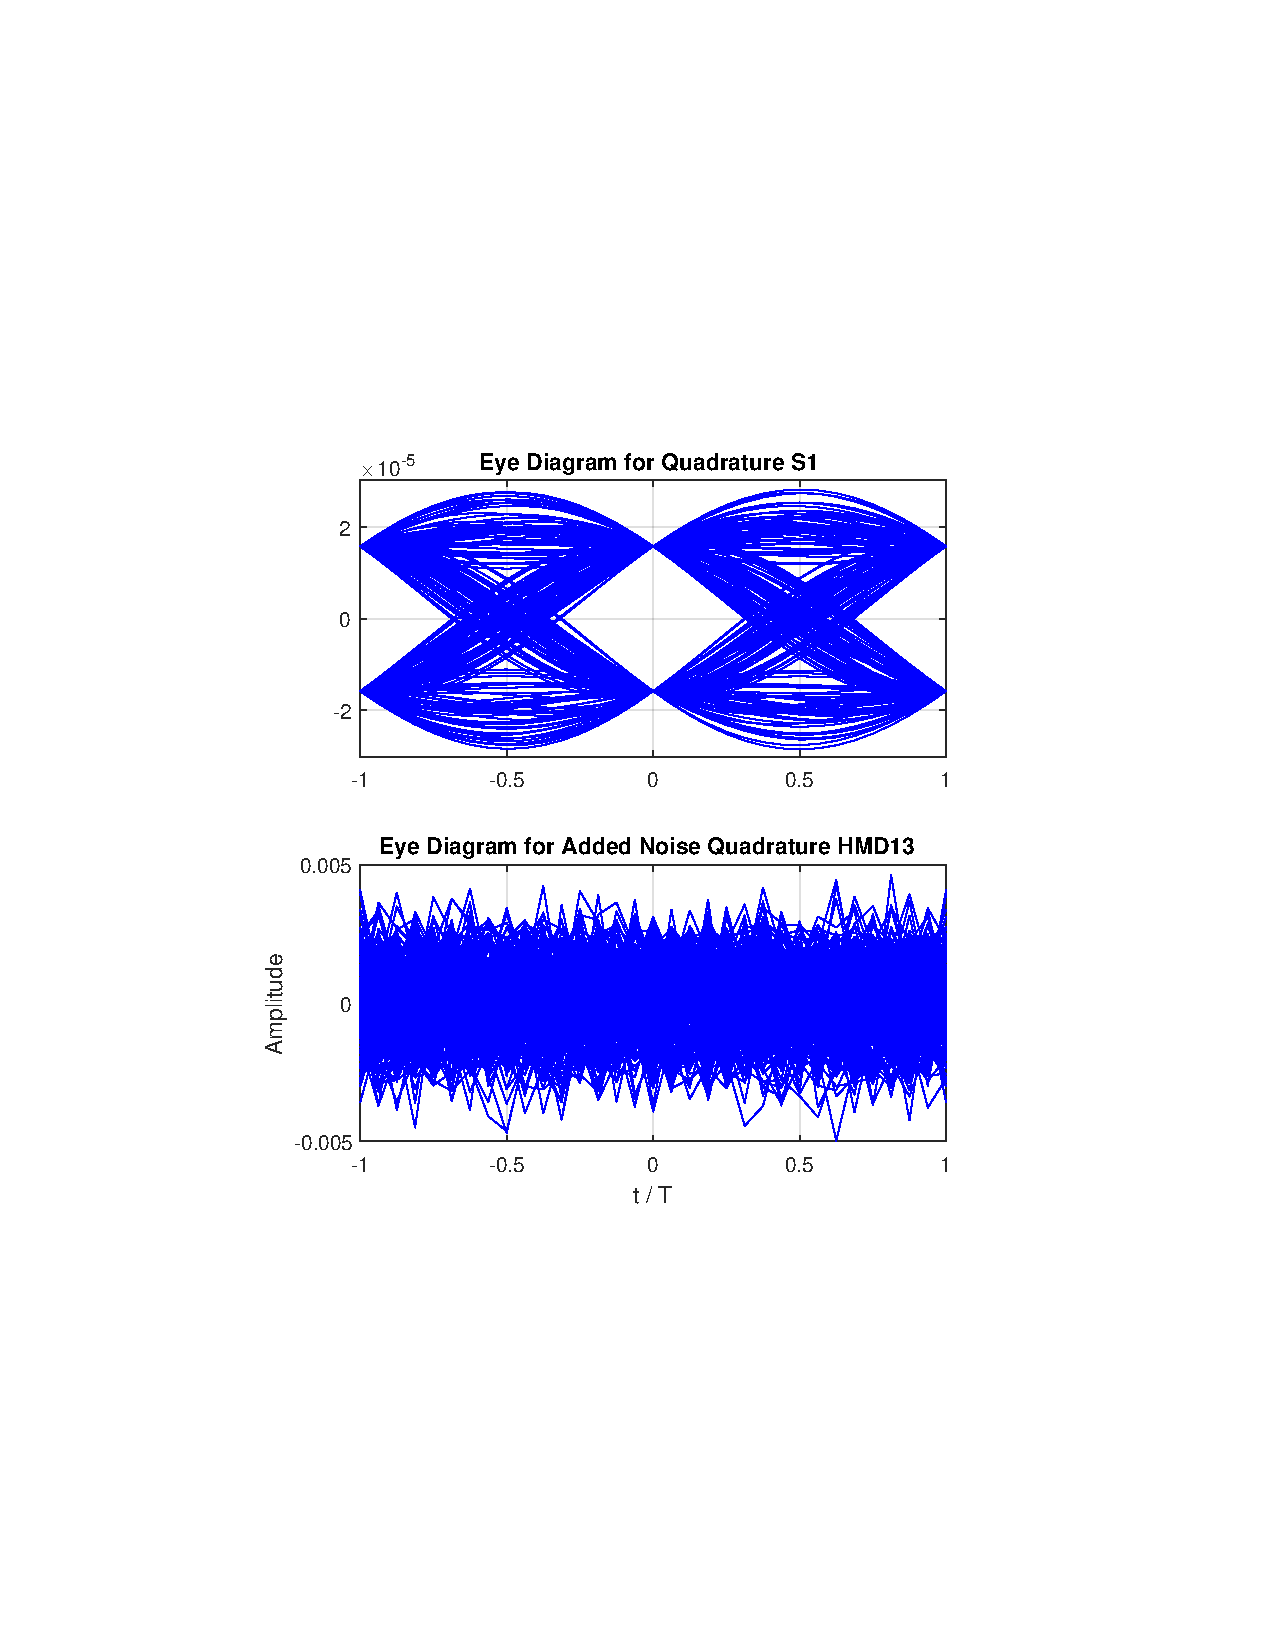
\includegraphics[clip, trim=5cm 4cm 5cm 4cm, width=\textwidth]{./sdf/m_qam_system/figures/eyes/q_n_nmf_60_60_rc_03.pdf}
	\end{subfigure}
	
	\caption{Eye diagrams without matched-filtering with raised-cosine at
		two different points: the optical output signal S1 on the top and the amplified
		signal with added noise at the middle, HMD12 and HMD13 for both components.
		Obtained through simulation with an optical power output of -60 dBm, 0 dBm at
		the local oscillator, a gain of $10^3$ at the amplifier, a noise spectral
		density of $10^{-6}$ and a rolloff factor of 0.3.\label{fig:eyes_n_rrc_60_03}}
	
\end{figure}

\begin{figure}[H]
	\centering
	\begin{subfigure}{.45\textwidth}
		\centering
		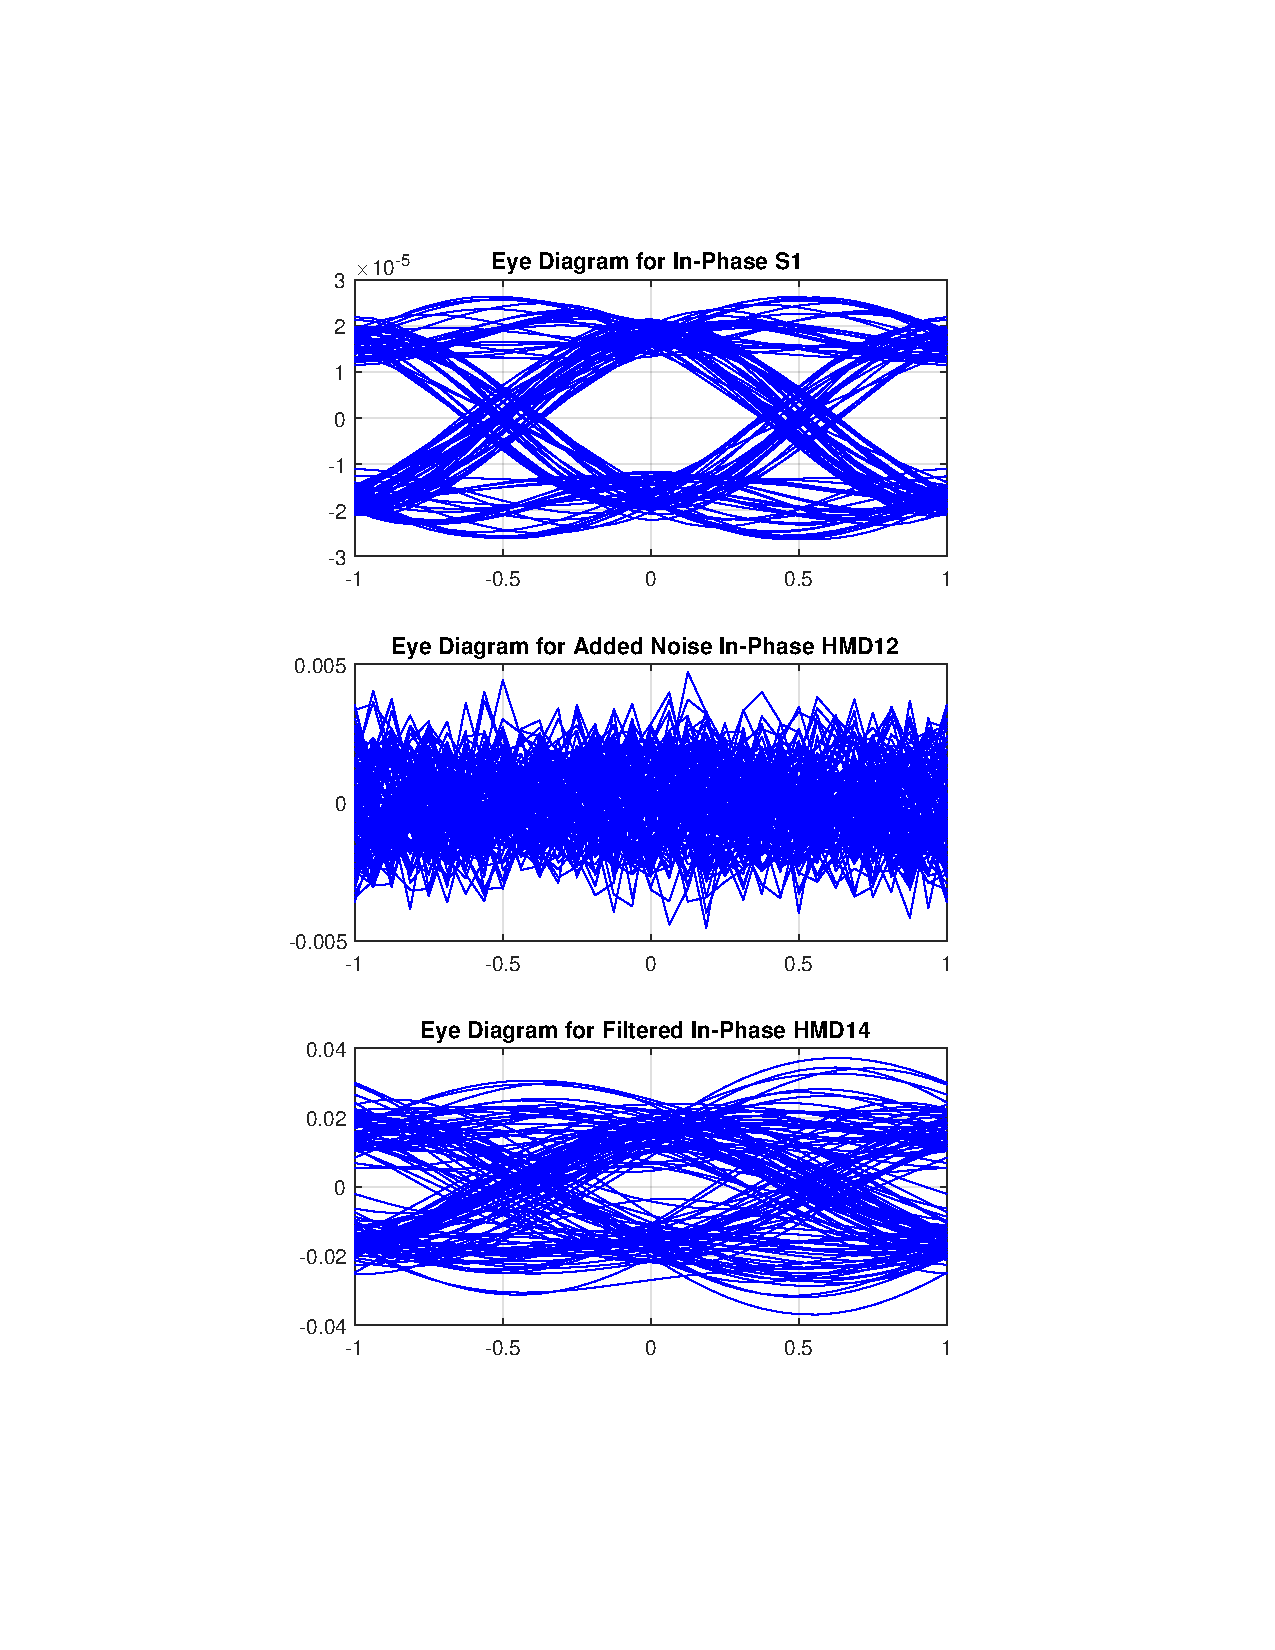
\includegraphics[clip, trim=5cm 4cm 5cm 4cm, width=\textwidth]{./sdf/m_qam_system/figures/eyes/if_p_60_03.pdf}
	\end{subfigure}
	\begin{subfigure}{.45\textwidth}
		\centering
		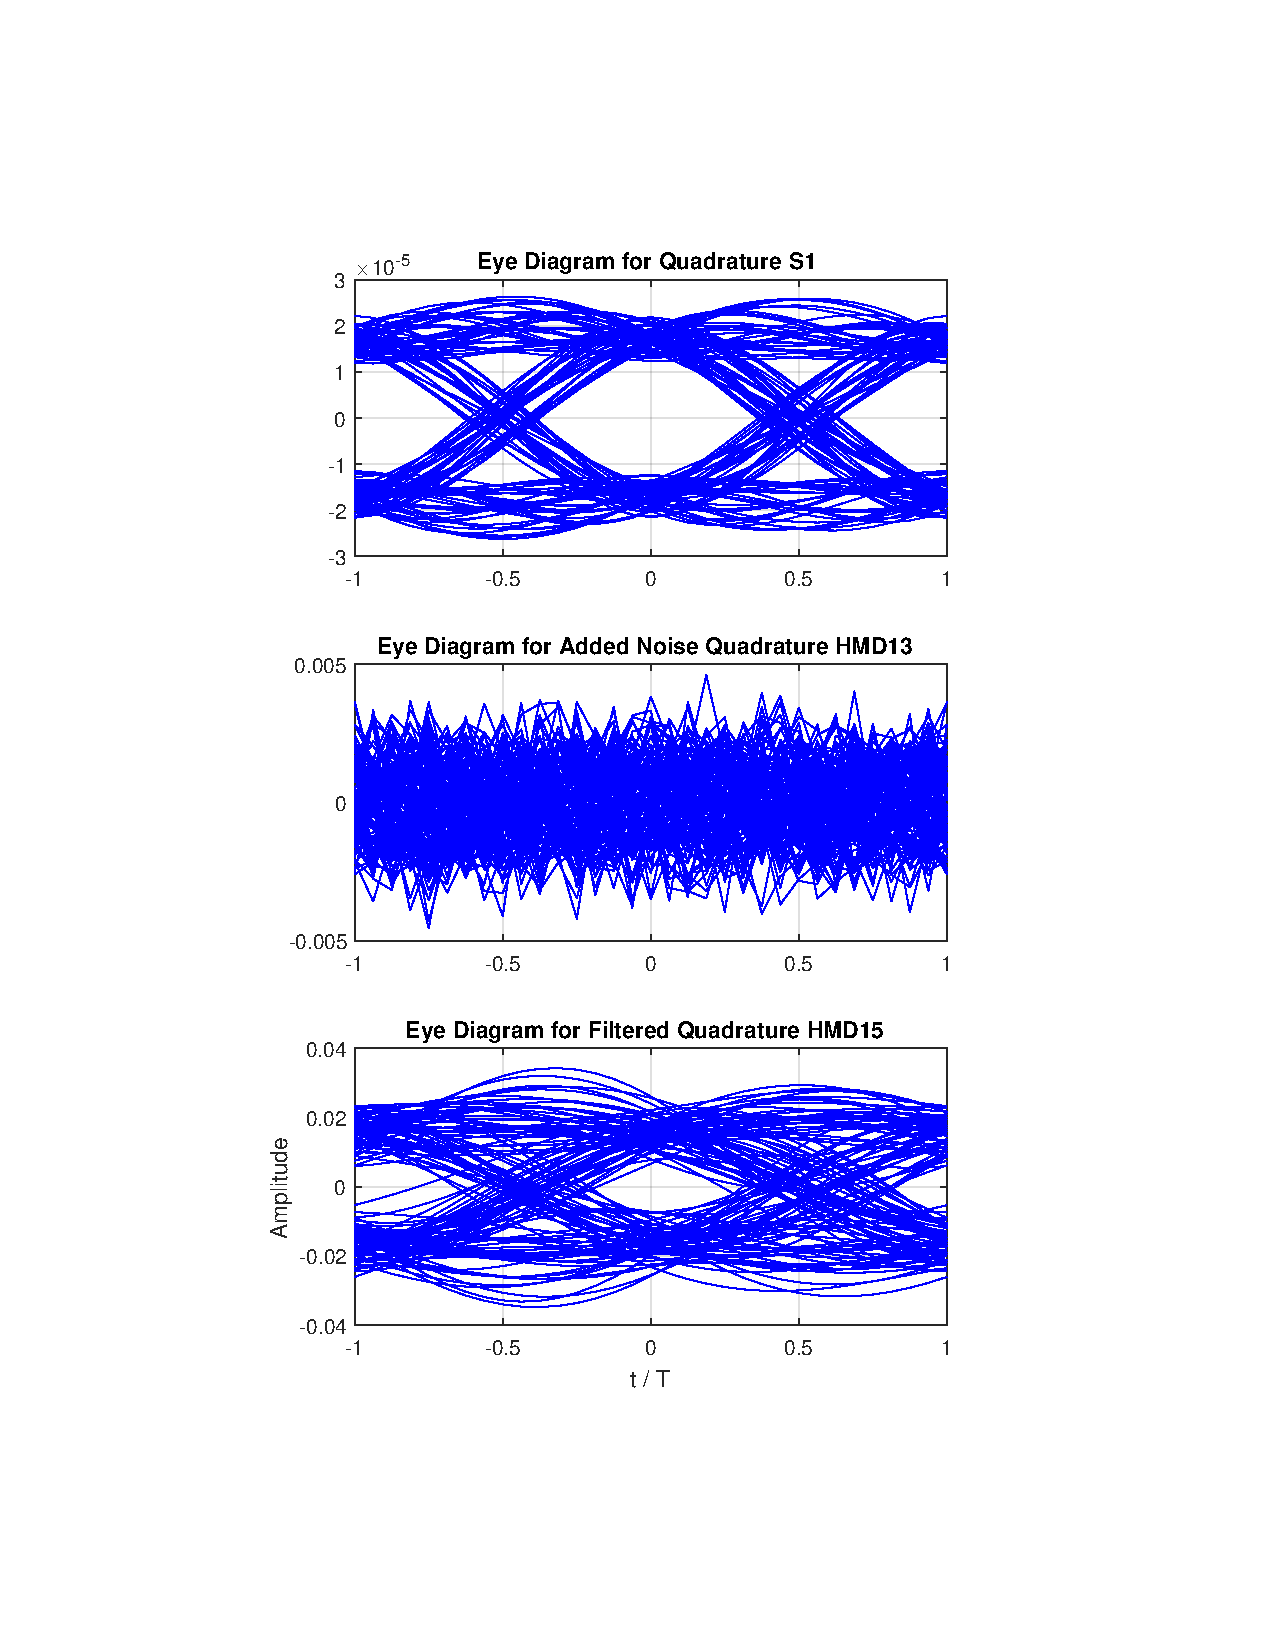
\includegraphics[clip, trim=5cm 4cm 5cm 4cm, width=\textwidth]{./sdf/m_qam_system/figures/eyes/q_p_60_03.pdf}
	\end{subfigure}
	
	\caption{Eye diagrams using matched filtering with root-raised-cosine
		at three different points: the optical output signal S1 on the top; the
		amplified signal with added noise at the middle, HMD12 and HMD13 for both
		components; and after passing through the last root-raised-cosine filter, HMD14
		and HMD15, for both components. Obtained through simulation with an optical
		power output of -60 dBm, 0 dBm at the local oscillator, a gain of $10^3$ at the
		amplifier, a noise spectral density of $10^{-6}$ and a rolloff factor of
		0.3.\label{fig:eyes_n_rc_60_03}} 
\end{figure}



\subsection{BER Curves}

The simulated results show agreement with the theoretical curves, as can be seen in Figure~\ref{fig:ber_pseudorandom}.
\begin{figure}[H]
	\centering
	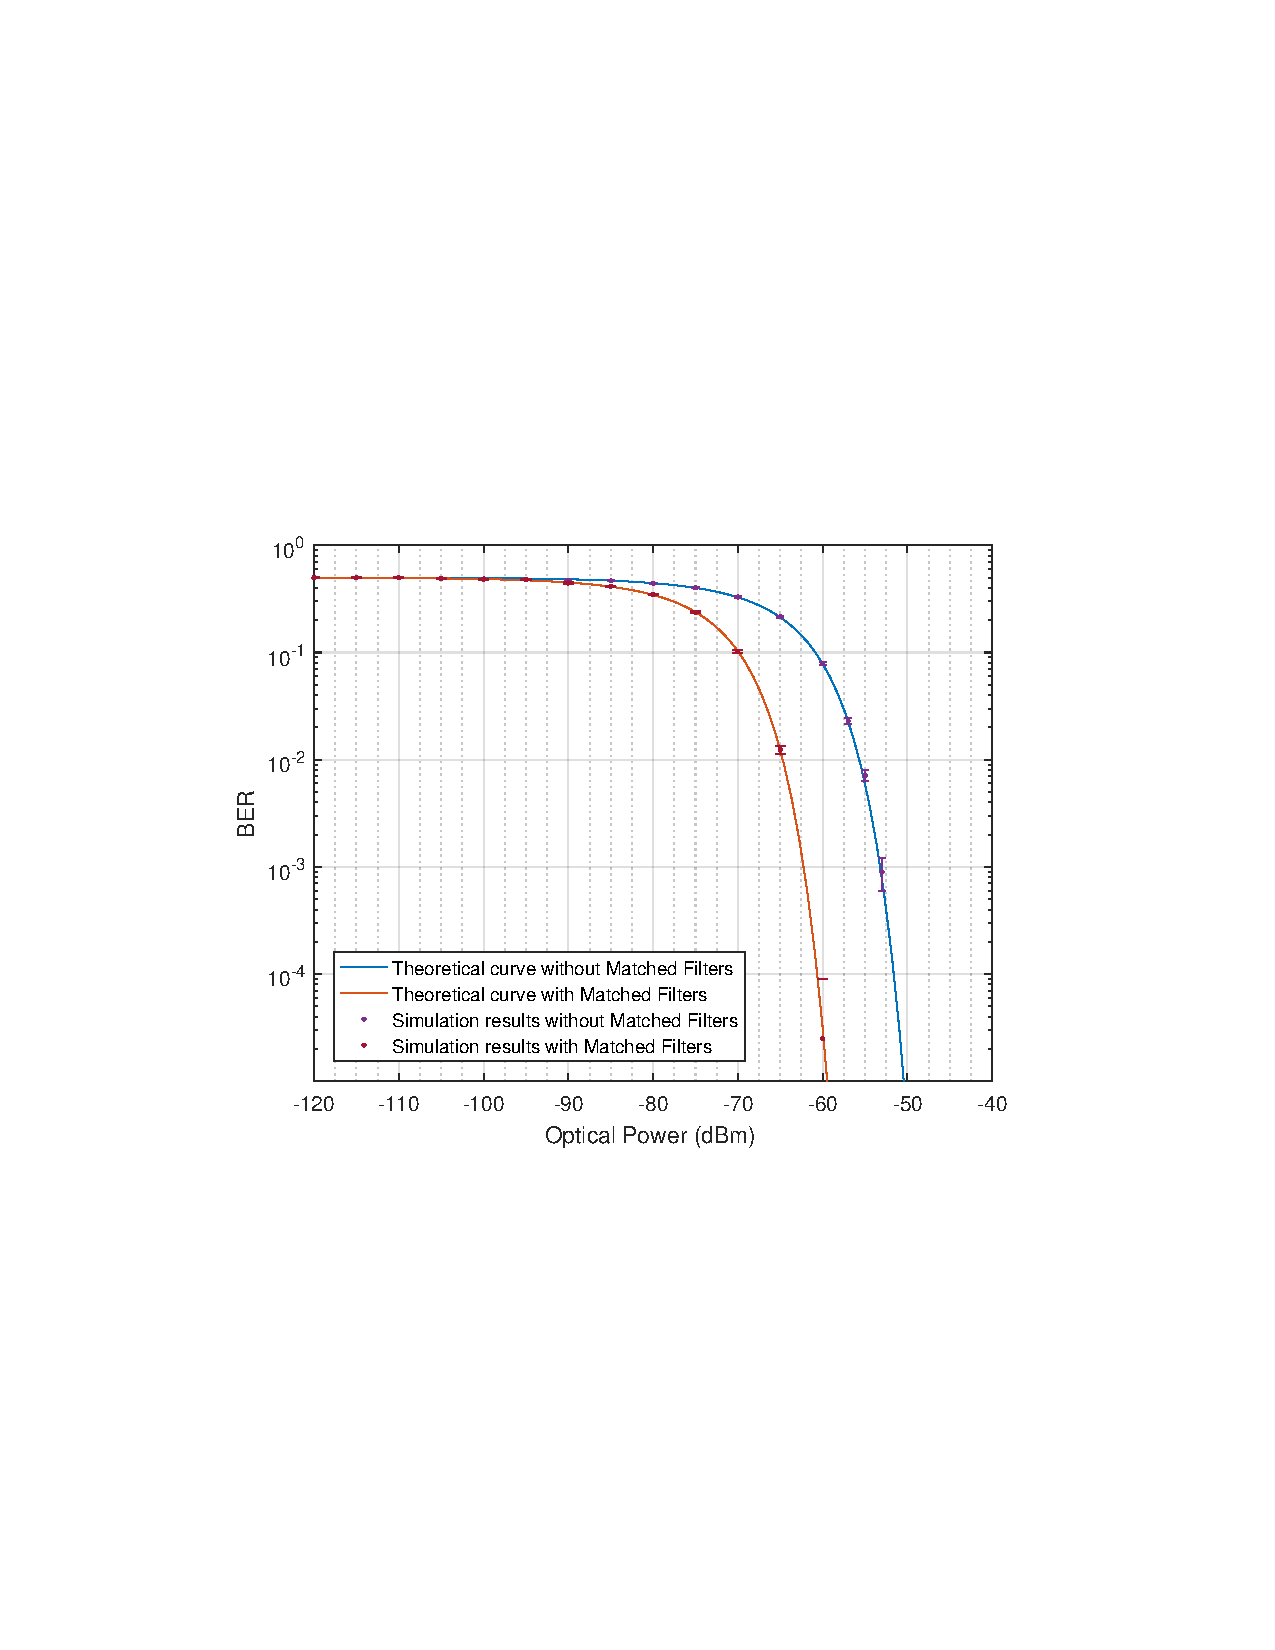
\includegraphics[clip, trim=4cm 8cm 4cm 8cm, width=0.7\textwidth]{./sdf/m_qam_system/figures/teor_vs_simul.pdf}
	\caption{Simulation results for a random binary sequence with $40000$ bits, a noise power of $10^{-6}$ and an amplification of $10^3$. The simulated values which used a matched filter were obtained by shaping the pulse with a root-raised-cosine FIR filter and filtering the signal before the sample with the same filter. The results without matched filtering were obtained by using shaping the pulses with a raised-cosine filter. The margins shown were obtained for a 95\% confidence level.}
	\label{fig:ber_pseudorandom}
\end{figure}% 

\subsubsection*{Conclusions}
The use of a root-raised-cosine filters for shaping and filtering the signal provides the best results, due to reducing noise while creating no inter-symbol interference. The experimental BER curves agree with the theoretical values and show the advantages of matched filtering.

\subsection*{Experimental Analysis}
\begin{figure}[H]
	\centering
	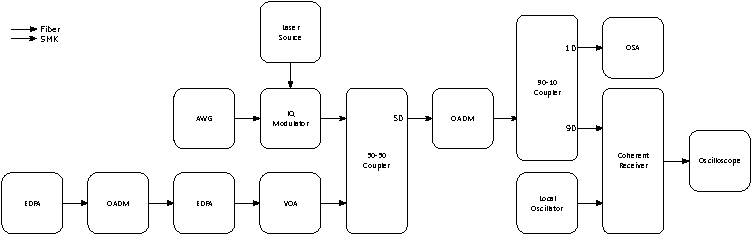
\includegraphics[width=\textwidth]{./sdf/m_qam_system/figures/mqamExperimental20180307.pdf}
	\caption{Experimental setup}
	\label{fig:experimental_mqam_setup}
\end{figure}
%
%
\begin{table}[H]
	\centering
	\begin{tabulary}{1.0\textwidth}{|L|L|l|}
%		\hline
%		\textbf{Device}		& \textbf{Description}\\
%		\hline
%		Balanced Photodetector	& Thorlabs PDB 450C\\
%		\hline
%%		BS					& Beam Splitter\\
%		\hline
%%		Pulse Generator		& HP 8116A Pulse Generator\\
%		\hline
%%		Amplitude Modulator	& Mach Zehnder SDL OC 48\\
%		\hline
%%		VOA					& Eigenlicht Power Meter 420\\
%		\hline
%%		VOA					& Thorlabs VOA 45-APC\\
%%		\hline
%%		PIN					& Thorlabs PDB 450C\\
%		\hline
%%		ADC					& Picoscope 6403D\\
%		\hline
	\end{tabulary}
\end{table}


\subsection{Comparative Analysis}

In this section we show the simulation results and compared them with the theoretical predictions for an M-QAM system with $M=4$. Figure \ref{fig:ber_pseudorandom} shows the variation of the BER with the optical power of the signal, using $40000$ bits produced by a random number generator. The noise power was set at $10^{-6}$, the local oscillator at $0~dBm$ and the amplification at the transimpedance amplifier was set at $10^3$.
The blue line represents the theoretical curve, while the orange points represent the simulated values with the respective confidence margins. The simulation agrees closely with the theoretical values.



%\begin{figure}[h]
%	\centering
%	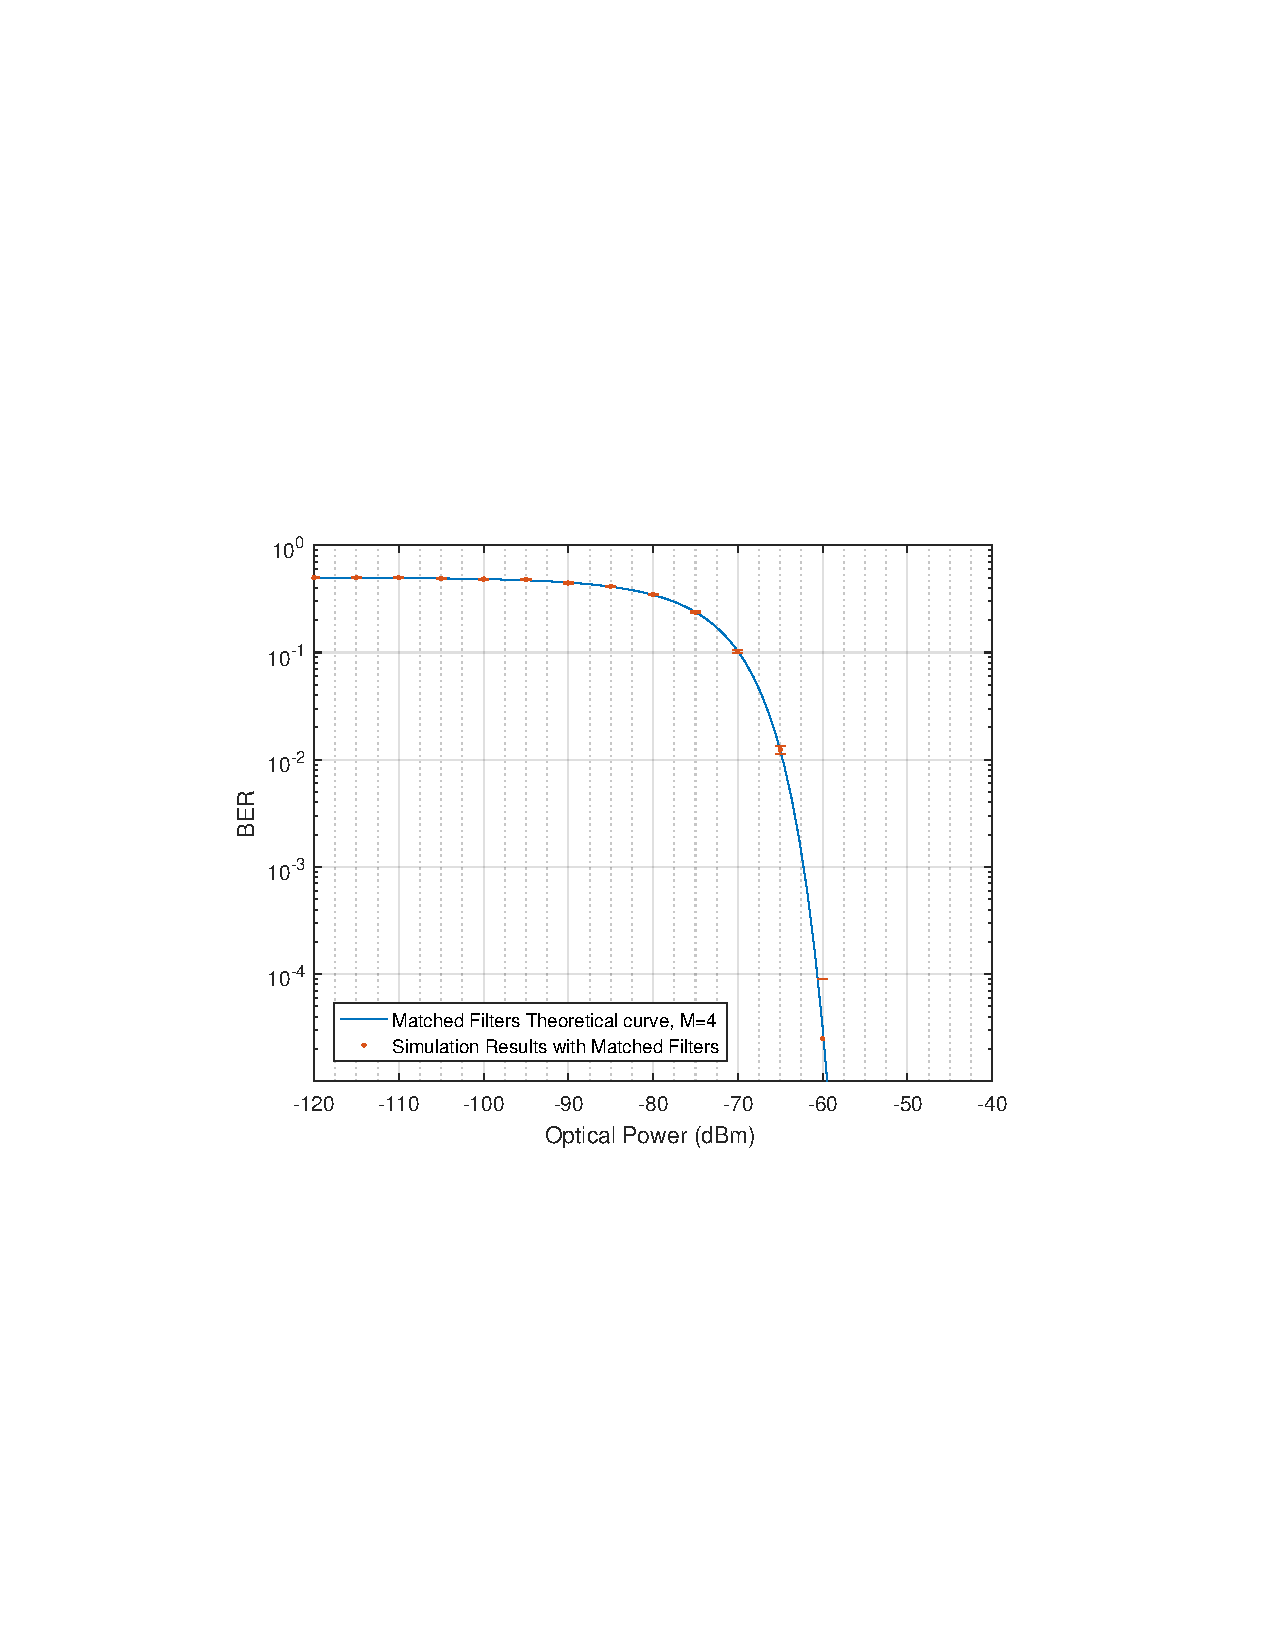
\includegraphics[clip, trim=4cm 8cm 4cm 8cm, width=0.7\textwidth]{./sdf/m_qam_system/figures/BER_QPSK_sim_mf_20180205.pdf}
%	\caption{Simulation result using root-raised cosine matched filtering for a random binary sequence with $40000$ bits, a noise power of $10^{-6}$ and an amplification of $10^3$.}
%	\label{fig:ber_pseudorandom_mf}
%\end{figure}% 


\subsection{Open Issues}

\newpage


%%%%%%%%%%%%%%%%%%%%%%%%%%%%%%%%%%%%%%%%%%%%%%%%%%%%%%%%%%%%%%%%%%%%%%%%%%%%%%%%%%%%%%%%%%%%%%%%%%%%%%%%%%%%
% References
%%%%%%%%%%%%%%%%%%%%%%%%%%%%%%%%%%%%%%%%%%%%%%%%%%%%%%%%%%%%%%%%%%%%%%%%%%%%%%%%%%%%%%%%%%%%%%%%%%%%%%%%%%%%

\renewcommand{\bibname}{References}
%
\bibliographystyle{myIEEEtran}
% argument is your BibTeX string definitions and bibliography database(s)
\bibliography{./sdf/m_qam_system/m_qam_system}
%
%


\cleardoublepage
